\documentclass [11pt, proquest] {thesis}[2015/03/03]
 
\setcounter{tocdepth}{1}  % Print the chapter and sections to the toc
 


% macros.tex
\usepackage{amsmath}
\usepackage{amsfonts}
\usepackage{amssymb}
\usepackage{amsthm}


% You change everything, by adding \usepackage{times} to the document
% Preamble. Now all the roman letters will be set in times and all the
% sans serif stuff will be set in Helvetica. If you don't like times,
% you can try the packages: palatcm, charter, helvet, palatino, avant,
% newcent and bookman
% If you want to change explicitly to a certain font, use the command
% \fontfamily{XYZ}\selectfont whereby XYZ can be set to: pag for Adobe
% AvantGarde, pbk for Adobe Bookman, pcr for Adobe Courier, phv for
% Adobe Helvetica, pnc for Adobe NewCenturySchoolbook, ppl for Adobe
% Palatino, ptm for Adobe Times Roman, pzc for Adobe ZapfChancery
\newcommand{\courier}{\fontfamily{pcr}\selectfont}



\newcommand{\edit}[1]{\footnote{[[#1]]}\marginpar{\hfill {\sf[[\thefootnote]]}}}
%\newcommand{\edit}[1]{{\sl\small [[Todo: #1]]}}


%\author{William~A. Stein}

\newcommand{\Hbar}{\overline{H}}

\newcommand{\myhead}[3]{
\par\noindent
{Version #2}
\vspace{10ex}
\par\noindent
{\bf \LARGE #1}\\
\vspace{3ex}
\par\noindent
{\large W.\thinspace{}A. Stein}\\
{\small Department of Mathematics, Harvard University}\vspace{1ex}\\
#3     
\vspace{2ex}\par
}

\newcommand{\myheadauth}[3]{
\par\noindent
{Version #2}
\vspace{10ex}
\par\noindent
{\bf \LARGE #1}\\
\vspace{3ex}
\par\noindent
#3     
\vspace{5ex}\par
}

\usepackage{xspace}  % to allow for text macros that don't eat space 
\newcommand{\SAGE}{{\sf Sage}\xspace}
\newcommand{\sage}{\SAGE}
\newcommand{\gzero}{\Gamma_0(N)}
\newcommand{\esM}{\overline{\sM}}
\newcommand{\sM}{\boldsymbol{\mathcal{M}}}
\newcommand{\sS}{\boldsymbol{\mathcal{S}}}
\newcommand{\sB}{\boldsymbol{\mathcal{B}}}       
\newcommand{\eE}{\mathbb{E}}
\newcommand{\bA}{\mathbb{A}}
\newcommand{\cK}{\mathcal{K}}
\newcommand{\Adual}{A^{\vee}}
\newcommand{\Bdual}{B^{\vee}}

\newcommand{\defn}[1]{{\em #1}}
\newcommand{\solution}[1]{\vspace{1em}%
  \par\noindent{\bf Solution #1.} }
\newcommand{\todo}[1]{\noindent$\bullet$ {\small \textsf{#1}} $\bullet$\\}
\newcommand{\done}[1]{\noindent {\small \textsf{Done: #1}}\\}
\newcommand{\danger}[1]{\marginpar{\small \textsl{#1}}}
\renewcommand{\div}{\mbox{\rm div}}
\DeclareMathOperator{\GCD}{GCD}
\DeclareMathOperator{\sss}{ss}
\renewcommand{\ss}{\sss}
\DeclareMathOperator{\red}{red}
\DeclareMathOperator{\sat}{sat}
\DeclareMathOperator{\xgcd}{xgcd}
\DeclareMathOperator{\Kol}{Kol}
\DeclareMathOperator{\can}{can}
\DeclareMathOperator{\Cl}{Cl}
\DeclareMathOperator{\Mod}{Mod}
\DeclareMathOperator{\chr}{char}
\DeclareMathOperator{\charpoly}{charpoly}
\DeclareMathOperator{\cris}{cris}
\DeclareMathOperator{\dR}{dR}
\DeclareMathOperator{\Fil}{Fil}
\DeclareMathOperator{\ind}{ind}
\DeclareMathOperator{\im}{im}
\DeclareMathOperator{\oo}{\infty}
\DeclareMathOperator{\abs}{abs}
\DeclareMathOperator{\lcm}{lcm}
\DeclareMathOperator{\cores}{cores}
\DeclareMathOperator{\coker}{coker}
\DeclareMathOperator{\image}{image}
\DeclareMathOperator{\prt}{part}
\DeclareMathOperator{\proj}{proj}
\DeclareMathOperator{\Br}{Br}
\DeclareMathOperator{\Ann}{Ann}
\DeclareMathOperator{\End}{End}
\DeclareMathOperator{\Tan}{Tan}
\DeclareMathOperator{\Eis}{Eis}
\newcommand{\unity}{\mathbb{1}}
\DeclareMathOperator{\Pic}{Pic}
\DeclareMathOperator{\Tate}{Tate}
\DeclareMathOperator{\Vol}{Vol}
\DeclareMathOperator{\Vis}{Vis}
\DeclareMathOperator{\Reg}{Reg}
%\DeclareMathOperator{\myRes}{Res}
%\newcommand{\Res}{\myRes}
\DeclareMathOperator{\Res}{Res}
\newcommand{\an}{{\rm an}}
\DeclareMathOperator{\rank}{rank}
\DeclareMathOperator{\Sel}{Sel}
\DeclareMathOperator{\Mat}{Mat}
\DeclareMathOperator{\BSD}{BSD}
\DeclareMathOperator{\id}{id}
\DeclareMathOperator{\dz}{dz}
%\DeclareMathOperator{\Re}{Re}
\renewcommand{\Re}{\mbox{\rm Re}}
\DeclareMathOperator{\Imm}{Im}
\renewcommand{\Im}{\Imm}
\DeclareMathOperator{\Selmer}{Selmer}
\newcommand{\pfSel}{\widehat{\Sel}}
\newcommand{\qe}{\stackrel{\mbox{\tiny ?}}{=}}
\newcommand{\isog}{\simeq}
\newcommand{\e}{\mathbf{e}}
\newcommand{\bN}{\mathbf{N}}

% ---- SHA ----
\DeclareFontEncoding{OT2}{}{} % to enable usage of cyrillic fonts
  \newcommand{\textcyr}[1]{%
    {\fontencoding{OT2}\fontfamily{wncyr}\fontseries{m}\fontshape{n}%
     \selectfont #1}}
\newcommand{\Sha}{{\mbox{\textcyr{Sh}}}}

%\font\cyr=wncyr10 scaled \magstep 1
%\font\cyr=wncyr10

%\newcommand{\Sha}{{\cyr X}}
\newcommand{\Shaan}{\Sha_{\mbox{\tiny \rm an}}}
\newcommand{\TS}{Shafarevich-Tate group}

\newcommand{\Gam}{\Gamma}
\newcommand{\X}{\mathcal{X}}
\newcommand{\cH}{\mathcal{H}}
\newcommand{\cA}{\mathcal{A}}
\newcommand{\cF}{\mathcal{F}}
\newcommand{\cG}{\mathcal{G}}
\newcommand{\cJ}{\mathcal{J}}
\newcommand{\cL}{\mathcal{L}}
\newcommand{\cV}{\mathcal{V}}
\newcommand{\cO}{\mathcal{O}}
\newcommand{\cQ}{\mathcal{Q}}
\newcommand{\cX}{\mathcal{X}}
\newcommand{\ds}{\displaystyle}
\newcommand{\M}{\mathcal{M}}
\newcommand{\E}{\mathcal{E}}
\renewcommand{\L}{\mathcal{L}}
\newcommand{\J}{\mathcal{J}}
\DeclareMathOperator{\new}{new}
\DeclareMathOperator{\Morph}{Morph}
\DeclareMathOperator{\old}{old}
\DeclareMathOperator{\Sym}{Sym}
\DeclareMathOperator{\Symb}{Symb}
%\newcommand{\Sym}{\mathcal{S}{\rm ym}}
\newcommand{\dw}{\delta(w)} 
\newcommand{\dwh}{\widehat{\delta(w)}}      
\newcommand{\dlwh}{\widehat{\delta_\l(w)}} 
\newcommand{\dash}{-\!\!\!\!-\!\!\!\!-\!\!\!\!-} 
\DeclareMathOperator{\tor}{tor}  
\newcommand{\Frobl}{\Frob_{\ell}}
\newcommand{\tE}{\tilde{E}}
\renewcommand{\l}{\ell}
\renewcommand{\t}{\tau}
\DeclareMathOperator{\cond}{cond}
\DeclareMathOperator{\Spec}{Spec}
\DeclareMathOperator{\Div}{Div}
\DeclareMathOperator{\Jac}{Jac}
\DeclareMathOperator{\res}{res}
\DeclareMathOperator{\Ker}{Ker}
\DeclareMathOperator{\Coker}{Coker}
\DeclareMathOperator{\sep}{sep}
\DeclareMathOperator{\sign}{sign}
\DeclareMathOperator{\unr}{unr}
\newcommand{\N}{\mathcal{N}}
\newcommand{\U}{\mathcal{U}}
\newcommand{\Kbar}{\overline{K}}
\newcommand{\Lbar}{\overline{L}}
\newcommand{\gammabar}{\overline{\gamma}}
\newcommand{\q}{\mathbf{q}}
%\renewcommand{\star}{\times}
\newcommand{\gM}{\mathfrak{M}}
\newcommand{\gA}{\mathfrak{A}}
\newcommand{\gP}{\mathfrak{P}}
\newcommand{\bmu}{\boldsymbol{\mu}}
\newcommand{\union}{\cup}
\newcommand{\Tl}{T_{\ell}}
\newcommand{\into}{\rightarrow}
\newcommand{\onto}{\rightarrow\!\!\!\!\rightarrow}
\newcommand{\intersect}{\cap}
\newcommand{\meet}{\cap}
\newcommand{\cross}{\times}
\DeclareMathOperator{\md}{mod}
\DeclareMathOperator{\toric}{toric}
\DeclareMathOperator{\tors}{tors}
\DeclareMathOperator{\Frac}{Frac}
\DeclareMathOperator{\corank}{corank}
\newcommand{\kr}[2]{\left(\frac{#1}{#2}\right)}
\newcommand{\rb}{\overline{\rho}}
\newcommand{\ra}{\rightarrow}
\newcommand{\xra}[1]{\xrightarrow{#1}}
\newcommand{\hra}{\hookrightarrow}
\newcommand{\la}{\leftarrow}
\newcommand{\lra}{\longrightarrow}
\newcommand{\riso}{\xrightarrow{\sim}}
\newcommand{\da}{\downarrow}
\newcommand{\ua}{\uparrow}
\newcommand{\con}{\equiv}
\newcommand{\Gm}{\mathbb{G}_m}
\newcommand{\pni}{\par\noindent}
\newcommand{\set}[1]{\left\{#1\right\}}
\newcommand{\iv}{^{-1}}
\newcommand{\alp}{\alpha}
\newcommand{\bq}{\mathbf{q}}
\newcommand{\cpp}{{\tt C++}}
\newcommand{\tensor}{\otimes}
\newcommand{\bg}{{\tt BruceGenus}}
\newcommand{\abcd}[4]{\left(
        \begin{smallmatrix}#1&#2\\#3&#4\end{smallmatrix}\right)}
\newcommand{\mthree}[9]{\left(
        \begin{matrix}#1&#2&#3\\#4&#5&#6\\#7&#8&#9
        \end{matrix}\right)}
\newcommand{\mtwo}[4]{\left(
        \begin{matrix}#1&#2\\#3&#4
        \end{matrix}\right)}
\newcommand{\vtwo}[2]{\left(
        \begin{matrix}#1\\#2
        \end{matrix}\right)}
\newcommand{\smallmtwo}[4]{\left(
        \begin{smallmatrix}#1&#2\\#3&#4
        \end{smallmatrix}\right)}
\newcommand{\twopii}{2\pi{}i{}}  
\newcommand{\eps}{\varepsilon}
\newcommand{\vphi}{\varphi}
\newcommand{\gp}{\mathfrak{p}}
\newcommand{\W}{\mathcal{W}}
\newcommand{\oz}{\overline{z}}
\newcommand{\Zpstar}{\Zp^{\star}}
\newcommand{\Zhat}{\widehat{\Z}}
\newcommand{\Zbar}{\overline{\Z}}
\newcommand{\Zl}{\Z_{\ell}}
\newcommand{\comment}[1]{}
\newcommand{\Q}{\mathbb{Q}}
\newcommand{\QQ}{\mathbb{Q}}
\newcommand{\GQ}{G_{\Q}}
\newcommand{\R}{\mathbb{R}}
\newcommand{\RR}{\mathbb{R}}
\newcommand{\PP}{\mathbb{P}}
\newcommand{\D}{{\mathbf D}}
\newcommand{\cC}{\mathcal{C}}
\newcommand{\cD}{\mathcal{D}}
\newcommand{\cP}{\mathcal{P}}
\newcommand{\cS}{\mathcal{S}}
\newcommand{\Sbar}{\overline{S}}
\newcommand{\K}{{\mathbb K}}
\newcommand{\C}{\mathbb{C}}
\newcommand{\CC}{\mathbb{C}}
\newcommand{\Cp}{{\mathbb C}_p}
\newcommand{\Sets}{\mbox{\rm\bf Sets}}
\newcommand{\bcC}{\boldsymbol{\mathcal{C}}}
\renewcommand{\P}{\mathbb{P}}
\newcommand{\Qbar}{\overline{\Q}}
\newcommand{\QQbar}{\overline{\Q}}
\newcommand{\kbar}{\overline{k}}
\newcommand{\dual}{\bot}
\newcommand{\T}{\mathbb{T}}
\newcommand{\TT}{\mathbb{T}}
\newcommand{\calT}{\mathcal{T}}
\newcommand{\cT}{\mathcal{T}}
\newcommand{\cbT}{\mathbb{\mathcal{T}}}
\newcommand{\cU}{\mathcal{U}}
\newcommand{\Z}{\mathbb{Z}}
\newcommand{\ZZ}{\mathbb{Z}}
\newcommand{\F}{\mathbb{F}}
\newcommand{\FF}{\mathbb{F}}
\newcommand{\Fl}{\F_{\ell}}
\newcommand{\Fell}{\Fl}
\newcommand{\Flbar}{\overline{\F}_{\ell}}
\newcommand{\Flnu}{\F_{\ell^{\nu}}}
\newcommand{\Fbar}{\overline{\F}}
\newcommand{\Fpbar}{\overline{\F}_p}
\newcommand{\fbar}{\overline{f}}
\newcommand{\Qp}{\Q_p}
\newcommand{\Ql}{\Q_{\ell}}
\newcommand{\Qell}{\Q_{\ell}}
\newcommand{\Qlbar}{\overline{\Q}_{\ell}}
\newcommand{\Qlnr}{\Q_{\ell}^{\text{nr}}}
\newcommand{\Qlur}{\Q_{\ell}^{\text{ur}}}
\newcommand{\Qltm}{\Q_{\ell}^{\text{tame}}}
\newcommand{\Qv}{\Q_v}
\newcommand{\Qpbar}{\Qbar_p}
\newcommand{\Zp}{\Z_p}
\newcommand{\Fp}{\F_p}
\newcommand{\Fq}{\F_q}
\newcommand{\Fqbar}{\overline{\F}_q}
\newcommand{\Ad}{Ad}
\newcommand{\adz}{\Ad^0}
\renewcommand{\O}{\mathcal{O}}
\newcommand{\A}{\mathcal{A}}
\newcommand{\Og}{O_{\gamma}}
\newcommand{\isom}{\cong}
\newcommand{\ncisom}{\approx}   % noncanonical isomorphism
\DeclareMathOperator{\ab}{ab}
\DeclareMathOperator{\alg}{alg}
\DeclareMathOperator{\Aut}{Aut}
\DeclareMathOperator{\Frob}{Frob}
\DeclareMathOperator{\Fr}{Fr}
\DeclareMathOperator{\Ver}{Ver}
\DeclareMathOperator{\Norm}{Norm}
\DeclareMathOperator{\Ind}{Ind}
\DeclareMathOperator{\norm}{norm}
\DeclareMathOperator{\disc}{disc}
\DeclareMathOperator{\ord}{ord}
\DeclareMathOperator{\GL}{GL}
\DeclareMathOperator{\PSL}{PSL}
\DeclareMathOperator{\PGL}{PGL}
\DeclareMathOperator{\Gal}{Gal}
\DeclareMathOperator{\SL}{SL}
\DeclareMathOperator{\SO}{SO}
\DeclareMathOperator{\WC}{WC}
\newcommand{\galq}{\Gal(\Qbar/\Q)}
\newcommand{\rhobar}{\overline{\rho}}
\newcommand{\cM}{\mathcal{M}}
\newcommand{\cB}{\mathcal{B}}
\newcommand{\cE}{\mathcal{E}}
\newcommand{\cR}{\mathcal{R}}
\newcommand{\et}{\text{\rm\'et}}

\newcommand{\sltwoz}{\SL_2(\Z)}
\newcommand{\sltwo}{\SL_2}
\newcommand{\gltwoz}{\GL_2(\Z)}
\newcommand{\mtwoz}{M_2(\Z)}
\newcommand{\gltwoq}{\GL_2(\Q)}
\newcommand{\gltwo}{\GL_2}
\newcommand{\gln}{\GL_n}
\newcommand{\psltwoz}{\PSL_2(\Z)}
\newcommand{\psltwo}{\PSL_2}
\newcommand{\h}{\mathfrak{h}}
\renewcommand{\a}{\mathfrak{a}}
\newcommand{\p}{\mathfrak{p}}
\newcommand{\m}{\mathfrak{m}}
\newcommand{\trho}{\tilde{\rho}}
\newcommand{\rhol}{\rho_{\ell}}
\newcommand{\rhoss}{\rho^{\text{ss}}}
\DeclareMathOperator{\tr}{tr}
\DeclareMathOperator{\order}{order}
\DeclareMathOperator{\ur}{ur}
\DeclareMathOperator{\Tr}{Tr}
\DeclareMathOperator{\Hom}{Hom}
\DeclareMathOperator{\Mor}{Mor}
\DeclareMathOperator{\HH}{H}
\renewcommand{\H}{\HH}
\DeclareMathOperator{\Ext}{Ext}
\DeclareMathOperator{\Tor}{Tor}
\newcommand{\smallzero}{\left(\begin{smallmatrix}0&0\\0&0
                        \end{smallmatrix}\right)}
\newcommand{\smallone}{\left(\begin{smallmatrix}1&0\\0&1
                        \end{smallmatrix}\right)}

\newcommand{\pari}{{\sc Pari}}
\newcommand{\magma}{{\sc Magma}}
\newcommand{\hecke}{{\sc Hecke}}
\newcommand{\lidia}{{\sc LiDIA}}

%%%% Theoremstyles
\theoremstyle{plain}
\newtheorem{theorem}{Theorem}[section]
\newtheorem{proposition}[theorem]{Proposition}
\newtheorem{corollary}[theorem]{Corollary}
\newtheorem{claim}[theorem]{Claim}
\newtheorem{lemma}[theorem]{Lemma}
\newtheorem{hypothesis}[theorem]{Hypothesis}
\newtheorem{conjecture}[theorem]{Conjecture}

\theoremstyle{definition}
\newtheorem{definition}[theorem]{Definition}
\newtheorem{question}[theorem]{Question}
\newtheorem{problem}[theorem]{Problem}
\newtheorem{openproblem}[theorem]{Open Problem}

%\theoremstyle{remark}
\newtheorem{goal}[theorem]{Goal}
\newtheorem{remark}[theorem]{Remark}
\newtheorem{remarks}[theorem]{Remarks}
\newtheorem{example}[theorem]{Example}
\newtheorem{exercise}[theorem]{Exercise}

\numberwithin{equation}{section}
\numberwithin{figure}{section}
\numberwithin{table}{section}


% bulleted list environment
\newenvironment{bulletlist}
   {
      \begin{list}
         {$\bullet$}
         {
            \setlength{\itemsep}{.5ex}
            \setlength{\parsep}{0ex}
            \setlength{\parskip}{0ex}
            \setlength{\topsep}{.5ex}
         }
   }
   {
      \end{list}
   }
%end newenvironment

% bulleted list environment
\newenvironment{dashlist}
   {
      \begin{list}
         {---}
         {
            \setlength{\itemsep}{.5ex}
            \setlength{\parsep}{0ex}
            \setlength{\parskip}{0ex}
            \setlength{\topsep}{.5ex}
         }
   }
   {
      \end{list}
   }
%end newenvironment

% numbered list environment
\newcounter{listnum}
\newenvironment{numlist}
   {
      \begin{list}
            {{\em \thelistnum.}}{
            \usecounter{listnum}
            \setlength{\itemsep}{.5ex}
            \setlength{\parsep}{0ex}
            \setlength{\parskip}{0ex}
            \setlength{\topsep}{.5ex}
         }
   }
   {
      \end{list}
   }
%end newenvironment

\newcommand{\hd}[1]{\vspace{1ex}\noindent{\bf #1} }
\newcommand{\nf}[1]{\underline{#1}} 
\newcommand{\cbar}{\overline{c}}

\DeclareMathOperator{\rad}{rad}

\theoremstyle{definition}
\newtheorem{algor}[theorem]{Algorithm}
\newenvironment{algorithm}[1]{%
\begin{algor}[#1]\index{{\bf Algorithm}!#1}
}%
{\end{algor}}

\newenvironment{steps}%
{\begin{enumerate}\setlength{\itemsep}{0.1ex}}{\end{enumerate}}

%\usepackage[hypertex]{hyperref}

%%% Local Variables: 
%%% mode: latex
%%% TeX-master: t
%%% End: 





%\usepackage{fullpage}
\usepackage{hyperref}
\usepackage{microtype}
\usepackage{mathtools}
\usepackage[usenames,dvipsnames]{color}
\usepackage[pdftex]{graphicx}
\usepackage{amsmath}
\usepackage{amssymb}
\usepackage{url}
%\usepackage{thmtools}
%\usepackage{thm-restate}

\includeonly{
chapters/1_introduction,
chapters/2_outline_and_results,
chapters/3_background,
chapters/4_main_theorem,
chapters/5_zero_sums,
chapters/6_remarks_future_work,
}

\newcommand{\NN}{\mathbb{N}}
\newcommand{\B}{\mathcal{B}}
\newcommand{\qedb}{\hfill $\blacksquare$}
\newcommand{\nrm}[1]{\left\|#1\right\|}
\newcommand{\pr}{^{\prime}}
\newcommand{\Les}{L_E(s)}
\newcommand{\Lams}{\Lambda_E(s)}
\newcommand{\Lfs}{L(f,s)}
\newcommand{\ldLes}{\frac{L_E\pr}{L_E}(s)}
\newcommand{\ldLfs}{\frac{L_f\pr}{L_f}(s)}
\newcommand{\ldLe}[1]{\frac{L_E\pr}{L_E}\left(#1\right)}
\newcommand{\ldLf}[1]{\frac{L_f\pr}{L_f}\left(#1\right)}
\newcommand{\ldLam}[1]{\frac{\Lambda_E\pr}{\Lambda_E}\left(#1\right)}
\newcommand{\ldatzero}{\frac{L\pr(E,0)}{L(E,0)}}
\newcommand{\xbar}{\overline{x}}
\newcommand{\ybar}{\overline{y}}
\newcommand{\AGM}{\text{AGM}}
\newcommand{\conj}[1]{\overline{#1}}
\newcommand{\EQ}{E(\QQ)}
\newcommand{\EFp}{E(\Fp)}
\newcommand{\Ensfpe}{E_{\text{ns}}(\FF_{p^e})}
\newcommand{\softO}{\tilde{O}}
\newcommand{\en}[1]{\lVert #1 \rVert}

\DeclareMathOperator{\Li}{Li}
\DeclareMathOperator{\sinc}{sinc}


\usepackage{alltt}  % 
\newenvironment{demo}
  {\begin{alltt}\leftskip3em
     \def\\{\ttfamily\char`\\}%
     \def\{{\ttfamily\char`\{}%
     \def\}{\ttfamily\char`\}}}
  {\end{alltt}}

\newtheorem{innercustomthm}{Theorem}
\newenvironment{quotedtheorem}[1]
  {\renewcommand\theinnercustomthm{#1}\innercustomthm}
  {\endinnercustomthm}
  
\newtheorem{innercustomcor}{Corollary}
\newenvironment{quotedcorollary}[1]
  {\renewcommand\theinnercustomcor{#1}\innercustomcor}
  {\endinnercustomcor}
  
\newtheorem{innercustomconj}{Conjecture}
\newenvironment{quotedconjecture}[1]
  {\renewcommand\theinnercustomconj{#1}\innercustomconj}
  {\endinnercustomconj}
 
% metafont font.  If logo not available, use the second form
%
% \font\mffont=logosl10 scaled\magstep1
\let\mffont=\sf
% --- end-of-sample-stuff ---
 

\begin{document}
 
% ==========   Preliminary pages
\prelimpages
 
%
% ----- copyright and title pages
%
\Title{The Zeros of Elliptic Curve $L$-functions: \\
Analytic Algorithms with Explicit Time Complexity}
\Author{Simon Spicer}
\Year{2015}
\Program{UW Mathematics}

\Chair{William Stein}{Professor}{Mathematics}
\Signature{Ralph Greenberg}
\Signature{Neal Koblitz}
\Signature{Bernard Deconinck, GSR}

\copyrightpage

% \titlepage  

% --- sample stuff only -----
% unusual footnote not found in a real thesis
% You just use the \titlepage as commented out above

{\Degreetext{A dissertation submitted in partial fulfillment \\of the requirements for the degree of}
 \def\thefootnote{\fnsymbol{footnote}}
 \let\footnoterule\relax
 \titlepage
 }
\setcounter{footnote}{0}

% --- end-of-sample-stuff ---
 
%
% ----- signature and quoteslip are gone
%

%
% ----- abstract
%
\setcounter{page}{-1}
\abstract{%
Elliptic curves are central objects of study in modern-day algebraic number theory. The problem of how to determine the rank of a rational elliptic curve is a difficult one, and at the time of the writing of this thesis an unconditional general method for doing so is not known. \\

It has been known for decades that contingent on the Birch and Swinnerton-Dyer Conjecture, an algorithm to compute rank exists, but this algorithm has unknown time complexity. In the first part of this thesis we prove that, assuming standard conjectures, an {\it effective} algorithm exists to compute rank with time complexity  that is polynomial in the curve's conductor. This method involves evaluating the $L$-function of the curve in question, and as such is practical for curves with conductors up to $\sim 10^{16}$ on current computer architecture. \\

The second part of this work addresses the question of what can be done when the conductor is too large for the above method to be practical. To this end we exhibit an analytic method to bound rank from above that doesn't rely on directly evaluating an elliptic curve's $L$-function, and as such can be used on curves with very large conductors. Because this method involves sums over the imaginary parts of the zeros of an elliptic curve $L$-function, we also include results concerning the locations thereof, and an exposition of related quantities.
}

\chapter*{Preface}
I have attempted to emphasize accessibility and readability throughout this work. Specifically, no knowledge beyond standard graduate-level complex analysis and algebra is assumed, and advanced knowledge of number theoretic topics is {\it not} required. As such, I hope that the results in this dissertation are accessible to a wide audience, even those at the advanced undergraduate level. Chapter 1 was written specifically to be a gentle introduction to the subject matter of this thesis. \\

For the expert I recommend skipping straight to Chapter 2, wherein the main results are stated. Proofs for these results can be found in Chapters 4 and 5 (from 5.2 onwards). \\

Finally, a note on conjecture dependencies. Many of the results in this work are contingent on the validity of three of the major open conjectures in number theory: the Birch and Swinnerton-Dyer conjecture (BSD), the Generalized Riemann Hypothesis (GRH) and the ABC conjecture (ABC). For ease of exposition, instead of stating explicitly in a result which of the above conjectures are assumed, we will list the three-letter initial of each assumed conjecture after the heading of each result. For example, the following result:
\begin{proposition}[BSD]
A rational elliptic curve with odd parity has a point of infinite order.
\end{proposition}
means that this proposition follows under the assumption that BSD is true.

%
% ----- contents & etc.
%
\tableofcontents
%\listoffigures
%\listoftables  % I have no tables
 
%%
%% ----- glossary 
%%
%\chapter*{Glossary}      % starred form omits the `chapter x'
%\addcontentsline{toc}{chapter}{Glossary}
%\thispagestyle{plain}
%%
%\begin{glossary}
%\item[argument] replacement text which customizes a \LaTeX\ macro for
%each particular usage.
%\item[back-up] a copy of a file to be used when catastrophe strikes
%the original.  People who make no back-ups deserve
%no sympathy.
%\item[control sequence] the normal form of a command to \LaTeX.
%\item[delimiter] something, often a character, that indicates
%the beginning and ending of an argument.
%More generally, a delimiter is a field separator.
%\item[document class] a file of macros that tailors \LaTeX\ for
%a particular document.  The macros described by this thesis
%constitute a document class.
%\item[document option] a macro or file of macros
%that further modifies \LaTeX\ for
%a particular document.  The option {\tt[chapternotes]}
%constitutes a document option.
%\item[figure] illustrated material, including graphs,
%diagrams, drawings and photographs.
%\item[font] a character set (the alphabet plus digits
%and special symbols) of a particular size and style.  A couple of fonts
%used in this thesis are twelve point roman and {\sl twelve point roman
%slanted}.
%\item[footnote] a note placed at the bottom of a page, end of a chapter,
%or end of a thesis that comments on or cites a reference
%for a designated part of the text.
%\item[formatter] (as opposed to a word-processor) arranges printed
%material according to instructions embedded in the text.
%A word-processor, on the other hand, is normally controlled
%by keyboard strokes that move text about on a display.
%\item[\LaTeX] simply the ultimate in computerized typesetting.
%\item[macro]  a complex control sequence composed of 
%other control sequences.
%\item[pica] an archaic unit of length.  One pica is twelve points and
%six picas is about an inch.
%\item[point] a unit of length.  72.27 points equals one inch.
%\item[roman]  a conventional printing typestyle using serifs.
%the decorations on the ends of letter strokes.
%This thesis is set in roman type.
%\item[rule] a straight printed line; e.g., \hrulefill.
%\item[serif] the decoration at the ends of letter strokes.
%\item[table] information placed in a columnar arrangement.
%\item[thesis] either a master's thesis or a doctoral dissertation.
%This document also refers to itself as a thesis, although it
%really is not one.
% 
%\end{glossary}
 
%
% ----- acknowledgments
%
\acknowledgments{
By no means did I produce this dissertation in a vacuum. Many individuals have provided critical contributions over the course of my studies, and we are thankful to all of them. However, some we must mention specifically. Sincere thanks must be given to my advisor William Stein, who for many years has provided the patient mentorship and guidance needed to make this dissertation a reality. I would also like to extend a heartfelt thanks to the University of Washington department of Mathematics as a whole, and to the graduate student coordinator Brooke Miller in particular, for supporting me throughout my studies at UW. \\

Beyond this, a number of mathematicians have given valuable advice. We are grateful for the correspondence with Barry Mazur on the explicit formula for elliptic curves, which was my entry point into the whole topic of elliptic curve $L$-functions; moreover we thank Peter Sarnak for his input on low-lying zeros of elliptic curve $L$-functions, and helping spur the formulation of the central idea of this thesis. John Cremona and Noam Elkies gave sage insight on the topics of the real period and regulator respectively. And we are grateful to John Voight, who used an early version of my rank estimation code and highlighted some significant bugs. And thanks must be given to Wei Ho, Jen Balakrishnan, Jamie Weigandt and Nathan Kaplan for putting up with my less-than-expert attempts to compute the ranks of large databases of elliptic curves. \\

And last but not least, a huge thank you to my wife Kimberly for her constant unwavering support throughout. 
}

%
% ----- dedication
%
\dedication{\begin{center}To Kimberly and Bram, who comprise two thirds of the Spicer Theorem.\end{center}}

%
% end of the preliminary pages
 
%
% ==========      Text pages
%
\textpages
 
% ========== Chapter 1
\chapter{Introduction}
% ----- CHAPTER 1: INTRODUCTION ----- %

Let $E$ be an elliptic curve over the rational numbers. We can think of $E$ as the set of rational solutions $(x,y)$ to a two-variable cubic equation in the form:
\begin{equation}
E: y^2 = x^3 + Ax + B
\end{equation}
for some integers $A$ and $B$, along with an extra "point at infinity". An important criterion is that the $E$ be a smooth curve; this translates to the requirement that the discriminant $D_E$ of the curve, given by $D_E = -16(4A^3+27B^2)$, is not zero.

One of the natural questions to ask when considering an elliptic curve is "how many rational solutions are there?" It turns out elliptic curves fall in that sweet spot where the answer could be zero, finitely many or infinitely many - and figuring out which is the case is a deeply non-trivial -- and as yet still open -- problem.

The rational solutions on $E$ form an abelian group with a well-defined group operation that can be easily computed. By a theorem of Mordell, the group of rational points on an elliptic curve $E(\mathbb{Q})$ is finitely generated; we can therefore write
\begin{equation}
E(\mathbb{Q}) \approx E_{\text{Tor}}(\Q) \times \mathbb{Z}^r,
\end{equation}
where $E_{\text{Tor}}(\Q)$ is a finite group (called the torsion subgroup of $E$), and $r$ is a non-negative integer, denoted the {\it algebraic rank} of $E$.

Determining the torsion subgroup of $E$ is relatively straightforward. By a celebrated theorem of Mazur, rational elliptic curves have torsion subgroups that are (non-canonically) isomorphic to one of precisely fifteen possibilities: $\mathbb{Z}/n\mathbb{Z}$ for $n = 1$ through $10$, or $\mathbb{Z}/12\mathbb{Z}$, or $\mathbb{Z}/2\mathbb{Z}\oplus \mathbb{Z}/2n\mathbb{Z}$ for $n = 1$ though $4$. However, computing the rank $r$ -- the number of independent rational points of infinite order on $E$ -- is hard, and no unconditional method to do so currently exists. It is towards this end that the work in this dissertation hopes to contribute. \\

Perhaps surprisingly, we can translate the algebraic problem of finding the number of rational solutions on $E$ to an analytic one -- at least conjecturally. The method of doing so is via elliptic curve $L$-functions; these are complex-analytic entire functions that somehow encode a great deal of information about the elliptic curve they describe. Unfortunately, it takes a few steps to define them:

\begin{definition}
Let $p$ be a prime number;
\begin{itemize}
\item Define $N_p(E)$ to be the number of points on the {\it reduced curve} $E$ modulo $p$. That is (excepting the cases $p=2$ or $3$, for which the definition is slightly more complicated), if $E$ has equation $y^2 = x^3 + Ax+B$, then
\begin{equation}
N_p(E) = 1 + \#\set{(\xbar,\ybar) \in \Fp^2 : \;\; \ybar \equiv \xbar^3 + A\xbar + B \;\;(\text{mod }p)},
\end{equation}
where the 1 accounts for the aforementioned point at infinity on $E$ not captured by the above equation.
\item Let $a_p(E) = p+1 - N_p(E)$.
\end{itemize}
\end{definition}
Hasse's Theorem states that $a_p(E)$ is always less that $2\sqrt{p}$ in magnitude for any $p$, and the Sato-Tate conjecure (recently proven by Taylor et al.) states that for a fixed elliptic curve, the $a_p$ values, once suitably normalized, are asymptotically distributed in a semi-circular distribution about zero. In other words, the number of solutions to an elliptic curve equation modulo $p$ is always about $p$, and can never be very far from that value.

\begin{definition}  For prime $p$,
\begin{itemize}
\item Define the {\it local factor} $L_p(E,s)$ to be the function of the complex variable $s$ as follows:
\begin{equation}
L_p(s) = \frac{1}{1-a_p(E)p^{-s} + \epsilon(p)p^{-2s}},
\end{equation}
where $\epsilon(p)$ is 0 if $p$ is a {\it prime of bad reduction}, and 1 otherwise. [For any elliptic curve $E$ there are only a finite number of primes of bad reduction; they are precisely the primes that divide the discriminant $D_E$ of a minimal model of $E$].
\item The {\bf (global) $L$-function $L(E,s)$ attached to $E$} is defined to be the product of all the local $L$-functions, namely
\begin{equation}
L(E,s)  = \prod_{p} L_p(E,s).
\end{equation}
\end{itemize}
\end{definition}
The above representation of $L(E,s)$ is called the Euler product form of the $L$-function. If we multiply out the terms and use power series inversion we can also write $L_E(s)$ as a {\it Dirichlet series}:
\begin{equation}
L(E,s) = \sum_{n=1}^{\infty} a_n(E) n^{-s},
\end{equation}
where for non-prime $n$ the coefficients $a_n$ are defined to be exactly the integers you get when you multiply out the Euler expansion.

If you do some analysis using Hasse's bound on the size of the $a_p(E)$ and their distribution according to Sato-Tate, one can show that the above two series converge absolutely when the real part of $s$ is greater than $\frac{3}{2}$ (see Lemma \ref{lem:ldLe_bound} and Corollary \ref{cor:L_E_abs_convergence}) and diverge when the real part of $s$ is less than $\frac{1}{2}$. However, the modularity theorem of Breuil, Conrad, Diamond, Taylor and Wiles \cite{BCDT-2011} \cite{TaWi-1995} \cite{Wil-1995} states that these elliptic curve $L$-functions can actually be analytically continued to the entire complex plane. That is, for every elliptic curve $L$-function $L(E,s)$ as defined above, there is an entire function on $\mathbb{C}$ which agrees with the Euler product/Dirichlet series definition for $\Re(s)>\frac{3}{2}$, but is also defined -- and explicitly computable -- for all other complex values of $s$. This entire function is what we actually call the $L$-function attached to $E$.

The way we analytically continue $L(E,s)$ yields that the function is highly symmetric about the line $\Re(s)=1$; moreover, because the function is defined by real coefficients $L_E(s)$ also obeys a reflection symmetry along the real axis. The point $s=1$ is therefore in a very real sense the {\it central point} for the $L$-function, and it is the behavior of $L(E,s)$ at the central point that conjecturally captures the rank information of $E$. This is established concretely in the Birch and Swinnerton-Dyer Conjecture, the first part of which we state below (the full conjecture is stated in Chapter 3):

\begin{conjecture}[Birch, Swinnerton-Dyer, part (a)]
Let $E$ be an elliptic curve over $\Q$, with attached $L$-series $L(E,s)$. Then the Taylor series expansion of $L_E(s)$ about the central point $s=1$ is
\begin{equation}
L(E,1+s) = Cs^r  + O(s^{r+1}),
\end{equation}
where
$C \ne 0$ and $r$ is the algebraic rank of $E$.
\end{conjecture}
That is, the first part of the BSD conjecture asserts that the order of vanishing of $L(E,s)$ at the central point is precisely the algebraic rank of $E$.

[Aside: Brian Birch and Peter Swinnerton-Dyer formulated the eponymous conjecture in the 1960s based in part on numerical evidence generated by the EDSAC computer at the University of Cambridge; this makes it one of the first instances of computer-generated data being used to support a mathematical hypothesis. Given the vast amount of supporting computational evidence that has now been collected, the BSD conjecture is overwhelmingly believed to be true.]

\begin{figure}[!h]
    \centering
    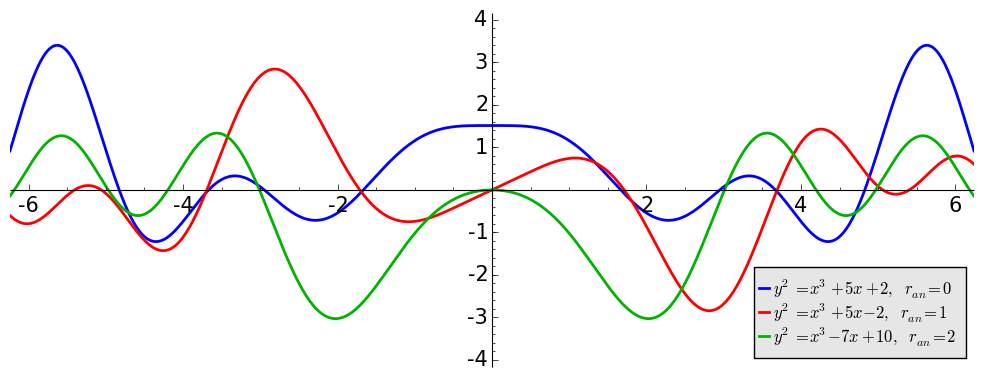
\includegraphics[width=1.0\textwidth]{graphics/L-functions_at_origin.png}
    \caption{The values of three elliptic curve $L$-functions along the critical line $1+it$ for $-6 \le t \le 6$, (transformed so that the functions are purely real to make the visualization a bit easier). Blue corresponds to a rank 0 curve, red is that of a rank 1 curve, and green is a rank 2 curve. Note that close to the origin the graphs look like non-zero constant function, a straight line and a parabola respectively.}
    \label{fig:L-functions_at_origin}
\end{figure}

We can therefore at least conjecturally determine the curve's algebraic rank by computing the order of vanishing of the elliptic curve's $L$-function at the central point. This converts an generally difficult algebraic problem into a perhaps more tractable analytic one.

The work in this thesis hopes to address the question of how to effectively compute the order of vanishing of $L(E,s)$ at $s=1$, which is denoted $r_{an}$, the {\it analytic rank} of $E$. This, again, is a non-trivial task -- for example, how do you numerically distinguish between the $n$th Taylor coefficient of $L(E,s)$ being identically zero, and it just being non-zero but so small in magnitude that it is indistinguishable from zero given your finite-precision computations?

The short answer is that, using a just a computer, you can't. We need theorems governing the magnitude of the Taylor coefficients -- especially that leading coefficient $C$ mentioned above -- in order to make analytic rank explicitly computable. This work establishes those results (assuming standard conjectures), telling us precisely how many digits of precision we need for an elliptic curve $L$-function to ascertain whether a given Taylor coefficient is or isn't zero. This in turn allows us to detail an algorithm to compute a curve's analytic rank with provable asymptotic time complexity . And thanks to the BSD conjecture, we therefore have a way to -- at least conjecturally -- compute the algebraic rank of $E$ with a concrete handle on how long the computation will take. \\

The phrases ``explicitly computable" and ``provable asymptotic time complexity" are given precise definitions in the main body of this thesis, so read on for a more formal statement of the main problem and results. \\

The structure of this dissertation is as follows: Chapter 2 more formally lays out the problem tackled in this work and quotes the major results obtained in this work. Chapter 3 consists of an exposition of the mathematical background relevant to this thesis; while chapter 4 contains proofs of the main results. Chapter 5 consists of analytic methods and results that allow one, for example, to obtain estimates on analytic rank when evaluating a curve's $L$-function directly is computationally infeasible. Chapter 6 consists of remarks and ideas for future work. Supporting computational evidence is supplied where relevant, as opposed to being collected in its own chapter. 
 
% ========== Chapter 2
\chapter{Problem Outline and Major Results}\label{sec:outline_results}
% ----- CHAPTER 2: PROBLEM OUTLINE AND RESULTS ----- %

A natural question to ask in the field of computational number theory is: does an algorithm exist to compute the rank of an elliptic curve? Manin showed in \cite{Man-1971} that, contingent on the Birch and Swinnerton-Dyer Conjecture being true, the answer to this question is yes. A rough outline of the method delineated by Manin is as follows: by day you search for points on a curve and thus obtain a lower bound on the algebraic rank of the curve; by night you evaluate central derivatives of the curve's $L$-function and thus obtain an upper bound on the analytic rank. If the Birch and Swinnerton-Dyer Conjecture is true, then eventually the two bounds will match up, and you will have computed the curve's rank. \\

However, although conjecturally guaranteed to terminate, the above method is ineffective from a time complexity perspective -- there are no results establishing just how long it will take for the two bounds to match up. It is thus a somewhat less than satisfying answer to the question posed. \\

We therefore modify the question to the following: given a rational elliptic curve $E$, does an algorithm exist to compute the rank of $E$ {\it that has provable big-Oh runtime in some measure of the arithmetic complexity of the curve}? In this work we answer this question in the affirmative. \\

The relevant measure of arithmetic complexity is the conductor $N_E$; below we provide an algorithm to compute rank and prove that it has polynomial runtime in $N_E$. However, to do so we must pay the price of having to assume not only the Birch and Swinnerton-Dyer Conjecture, but also the ABC Conjecture. The algorithm can be further sped up by assuming the Generalized Riemann Hypothesis. From hereon out we refer to these three big conjectures as BSD, ABC and GRH respectively. \\

Specifically, we establish the following result:
\begin{theorem}\label{thm:main_theorem}
Let $E/\QQ$ have conductor $N_E$. Contingent on BSD and ABC, there exists an algorithm to compute the algebraic rank $r_E$ of $E$ in $\softO\left(\sqrt{N_E}\right)$ time and $\softO(1)$ space. That is, for any $\epsilon>0$ the algorithm is guaranteed to terminate with a correct output in $O\left((N_E)^{\frac{1}{2}+\epsilon}\right)$ time, using only $O\left((N_E)^{\epsilon}\right)$ space.
\end{theorem}
The algorithm in question is as follows:
\begin{algorithm}{Compute the rank of an elliptic curve}\label{algo:compute_rank}
Given a rational elliptic curve $E$ represented by a global minimal Weierstrass equation $y^2 + a_1 xy + a_3 y^2 = x^3 + a_2 x^2 + a_4 x + a_6$ with known conductor $N_E$:
\begin{steps}
\item Compute the real period $\Omega_E$ of $E$.
\item Set $k = 65 + 10.5 \log_2 N_E - \log_2 \Omega_E$, and set $m=0$.
\item Evaluate $\frac{L_E^{(m)}(1)}{m!}$, the $m$th Taylor coefficient of the $L$-function of $E$ at the central point, to $k$ bits precision. If all $k$ bits are zero, increment $m$ by 1 and repeat this step.
\item Output $r_E=m$ and halt.
\end{steps}
\end{algorithm}

Furthermore, if one also assumes GRH, step 2. can be replaced with:
\begin{enumerate}
\item[2.] Set $k = 31 + 6.7 \log_2 N_E - \log_2 \Omega_E$, and set $r=0$.
\end{enumerate}
This will reduce the runtime of Algorithm \ref{algo:compute_rank} by a constant factor. \\

This algorithm is not new -- it is just a refinement on bounding the analytic rank of a curve with an explicitly chosen precision. What {\it is} new is the body of results in this dissertation proving that, assuming BSD and ABC (and optionally GRH), if the $m$th derivative of the $L$-series attached to $E$ is zero to $k$ bits precision, then it {\it is} identically zero. This allows us to convert an algorithm that a priori only provides upper bounds on analytic rank, to one that computes rank exactly. Furthermore, we show that the algorithm is guaranteed to terminate in time polynomial in the curve's conductor. \\

Moreover, Algorithm \ref{algo:compute_rank} is in a sense optimal among analytic rank computation methods: since evaluating $\Les$ takes $\tilde{O}(\sqrt{N_E})$ time, we cannot hope to get the rank out in time faster than this. [Of course other rank computation methods do exist, but they don't involve working with $\Les$ directly.] The proof of Theorem \ref{thm:main_theorem} can be found in section \ref{sec:main_thrm_proof}, but will require results established in preceding and following sections. \\

This work includes a number of related results; we quote below a selection which we believe are of particular interest:

\begin{corollary}[\ref{cor:real_period_upper_bound}] 
For $E/\QQ$ with real period $\Omega_E$ and conductor $N_E$,
\begin{equation}
\Omega_E < 8.82921517\ldots \cdot (N_E)^{-\frac{1}{12}}
\end{equation}
That is, the real period goes to zero as the conductor of the curve goes to infinity. This result is unconditional.
\end{corollary}

\begin{theorem}[\ref{thm:zero_density}]
Let $E$ have conductor $N_E$, and let $M_E(t)$ count the number of nontrivial zeros of $\Les$ with imaginary part at most $t$ in value. Then contingent on GRH, for $t>>0$ we have
\begin{equation}\label{eqn:zero_density}
M_E(t) = \frac{t}{\pi} \, \log\left(\frac{t\sqrt{N_E}}{2\pi e}\right) + \frac{1}{4} + O(\log t),
\end{equation}
where the error term is positive as often as it negative and contributes no net bias asymptotically.
\end{theorem}

\begin{corollary}[\ref{cor:gamma_n_approx_value}]
Let $\gamma_n := \gamma_n(E)$ be the imaginary value of the $n$th nontrivial (and noncentral) zero in the upper half plane of $\Les$ with analytic rank $r_E$.  Moreover, let $W_0 (s)$ be the Lambert W-function on $\CC$ i.e. the principal branch of the functional inverse of $s e^s$. Then contingent on GRH, for $n >> 1$ we have
\begin{equation}
\gamma_n = \frac{2\pi e}{\sqrt{N_E}} \cdot \exp \left(W_0\left[\left(\frac{r_E}{2} +n - \frac{3}{4}\right)\cdot \frac{\sqrt{N_E}}{2 e}\right]\right) + O(\log n)
\end{equation}
where the error term is positive as often as it negative and contributes no net bias asymptotically.
\end{corollary}

\begin{corollary}[\ref{cor:sinc_squared_sum_with_bite}]
Let $E/\QQ$ have analytic rank $r_E$, conductor $N_E$ and bite $\beta_E$. Then contingent on GRH, $r_E$ is the largest integer less than the quantity
\begin{equation}
\frac{1}{\sqrt{\beta_E}}\left[\left(-\eta + \log\left(\frac{\sqrt{N_E}}{2\pi}\right)\right)+ \frac{1}{2 \sqrt{\beta_E}}\left(\frac{\pi^2}{6} - \Li_2\left(e^{-2\sqrt{\beta_E}}\right)\right) + \sum_{\log n<2\sqrt{\beta_E}} c_n(E) \cdot \left(1-\frac{\log n}{2\sqrt{\beta_E}}\right)\right]
\end{equation}
where $Li_2(s)$ is the dilogarithm function on $\CC$, and $c_n(E)$ is the $n$th Dirichlet coefficient of $\ldLe{1+s}$.
\end{corollary}

The next chapter provides definitions and background theory for the quantities mentioned in the results above; the the proofs can of course be found in the respective sections later in this work.


 
% ========== Chapter 3 
\chapter{Notation, Definitions and Background}\label{sec:defs_background}
% ----- CHAPTER 3: NOTATION, DEFINITIONS AND BACKGROUND ----- %

%%%%%%%%%%%%%%%%%%%%%%%%%%
\section{Notation}\label{subsec:notation}

For the rest of the body of this text we set the following notation:
\begin{itemize}
\item $E$ is an elliptic curve over $\QQ$ given by minimal Weierstrass equation
\begin{equation*}
y^2 + a_1 xy + a_3 y^2 = x^3 + a_2 x^2 + a_4 x + a_6,
\end{equation*}
 where $a_1, a_3 \in \set{0,1}$, $a_2 \in \set{-1,0,1}$ and $a_4,a_6 \in \ZZ$.
\item $D(E)$, $N(E)$ and $r_{al}(E)$  and $r_{an}(E)$ are the discriminant, conductor, algebraic rank and analytic rank of $E$ respectively. For ease of exposition, the dependence on $E$ will most often be indicated by a subscript $E$ instead, and when there is no ambiguity it may be dropped entirely. Also, since much of this body of work assumes the validity of the the BSD conjecture, the algebraic and analytic rank of a curve will most often be assumed to be equal, in which case it will just be denoted $r_E$.
\item $p$ is a (rational) prime number and $q$ is a prime power.
\item $s$ is the generic complex variable.
\item $L(E,s)$ and $\Lambda(E,s)$ are the standard and completed $L$-functions attached to $E$ respectively. Again, for ease of exposition we will in general subsume the $E$ into a subscript and write $\Les$ and $\Lams$.
\item $C(E) = C_E$ is the leading nonzero coefficient of the Taylor series of $\Lambda_E(s)$ about $s=1$; \\
$C\pr(E) = C\pr_E$ is the leading nonzero coefficient of the Taylor series of $L_E(s)$ about $s=1$.
\item $\gamma$ will always be used to denote the imaginary parts of nontrivial zeros of an $L$-function.
\item $\beta(E) = \beta_E$ is the bite of $E$, defined as $\beta_E = \sum_{\gamma\ne 0} \gamma^{-2}$, where $\gamma$ ranges over the noncentral nontrivial zeros of $\Les$.
\item $\eta$ is the Euler-Mascheroni constant $= 0.5772156649\ldots$
\item $\Gamma(s)$ is the standard Gamma function on $\CC$, and the digamma function: $\digamma(s) = \frac{\Gamma\pr}{\Gamma}(s)$ is the logarithmic derivative of $\Gamma(s)$.
\end{itemize}

Furthermore, we define the following values associated to $E$ (in all cases the dependence on $E$ is understood):
\begin{itemize}
\item $b_2 = a_1^2 + 4a_2$
\item $b_4 = a_1 a_3 + 2a_4$
\item $b_6 = a_3^2 + 4a^6$
\item $b_8 = a_1^2 a_6 + 4 a_2 a_6 - a_1 a_3 a_4 + a_2 a_3^2 - a_4^2$
\item $c_4 = b_2^2 - 24 b_4$
\item $c_6 = -b_2^3 + 36 b_2 b_4  - 216 b_6$
\item $D = D(E) = -b_2^2 b_8 - 8 b_4^3 - 27 b_6^2 + 9 b_2 b_4 b_6$; this is the definition of the discriminant of $E$
\item $j = j(E) = \frac{c_4}{D}$ is the $j$-invariant of $E$
%\item $\omega = \frac{dx}{2y + a_1 x + a_3} = \frac{dy}{3x^2 + 2a_2 x + a_4 - a_1 y}$
\end{itemize}

\newpage
%%%%%%%%%%%%%%%%%%%%%%%%%%
\section{Definitions and Basic Results}

The rest of this chapter covers the basic definitions of and results needed for the rest of this work (namely, big-Oh notation, elliptic curves and $L$-functions). Feel free to skip this if you are familiar with them.

%%%%%%%%%%%%
\subsection{Big-Oh Notation}

Given that the running time of various algorithms will be discussed over the course of this work, we recall the definitions of big-Oh and soft-Oh notation, at least in the context of how they will be used here.

\begin{definition}
Let $x$ be a positive input, and let $g(x)$ be some positive-valued reference function on $x$.
\begin{itemize}
\item We say a function $f(x) = O(g(x))$ (read ``$f$ is big-Oh of $g$''), if
\begin{equation}
\limsup_{x \to \infty} \left| \frac{f(x)}{g(x)}\right| < \infty.
\end{equation}
That is, $f(x) = O(g(x))$ if the asymptotic growth/decay rate of $f$ is bounded by some multiple of that of $g$.
\item We say a function $f(x) = \softO(g(x))$ (read ``$f$ is soft-Oh of $g$''), if there is some $m>0$ such that
\begin{equation}
\limsup_{x \to \infty} \left| \frac{f(x)}{g(x)\left(\log g(x)\right)^m}\right| < \infty.
\end{equation}
That is, $f(x) = \softO(g(x))$ if the asymptotic growth/decay rate of $f$ scales like that of $g$, up to the inclusion of log factors.
\end{itemize}
\end{definition}
Note that $f(x) = \softO(g(x))$ implies that $f(x) = O(g(x)^{1+\epsilon})$ for any $\epsilon>0$, but not vice versa; there are complexity classes strictly between the two. In this thesis we will work exclusively with soft $O$ time complexities, so there is no need to elaborate on those classes here.\\

\begin{definition}
Let $A$ be an algorithm which takes input of size $k$, where for simplicity we may think of $k$ as a positive integer. Let $t_A(k)$ be the running time of $A$ thought of as a function of the input size $k$.
\begin{itemize}
\item $A$ is said to have {\it polynomial time complexity} if there is some $m>0$ such that the running time of $t_A(k) = O(k^{m})$, i.e. the asymptotic running time of the algorithm scales like some polynomial function of $k$.
\item If $t_A(k) = O(k^{\epsilon})$ for any $\epsilon>0$, then $A$ is said to have {\it sub-polynomial time complexity}. Note that if $t_A(k) = \softO(1)$, then $A$ has sub-polynomial time complexity.
\item If no $m>0$ exists such that $t_A(k) = O(k^m)$, then $A$ is said to have {\it super-polynomial time complexity}. If there is some $m>1$ such that $t_A(k) = O(m^k)$, then $A$ is said to have {\it exponential time complexity}.
\end{itemize}
\end{definition}
Again, there are complexity classes strictly between polynomial and exponential complexity, but we won't consider them in this thesis. The same terminology can be applied to the space requirements of an algorithm, wherein we would replace the word `time' with `space'. \\

Note that in theoretical computer science the $k$ is typically the number of bits needed to specify the input to the algorithm. However, in computational number theory the input itself is often a positive integer; many algorithms scale with some polynomial of the input magnitude as opposed to the number of bits defining the input. We therefore highlight the distinction between ``polynomial time in the number of bits of the input" and ``polynomial time in the magnitude of the input": the former is asymptotically much faster than the latter. When discussing time complexities we will always be clear to delineate what the measure of complexity $k$ is. \\



%%%%%%%%%%%%
\subsection{Elliptic curves}

\begin{definition}
An elliptic curve $E$ is a genus 1 smooth projective curve with a marked point $\cO$. $E$ is defined over a field $K$ if $E$ may be represented by the {\it Weierstrass equation} $y^2 + a_1 xy + a_3 y^2 = x^3 + a_2 x^2 + a_4 x + a_6$, where $a1,\ldots a_6 \in K$.
\end{definition}

For elliptic curves defined over $\QQ$, we may always find a model for $E$ such that $a_1, a_3 \in \set{0,1}$, $a_2 \in \set{-1,0,1}$ and $a_4,a_6 \in \ZZ$. Furthermore, there is the notion of {\it minimality} when it comes to models for elliptic curves. Without going into the definition thereof, unless stated otherwise we will assume that any given elliptic curve Weierstrass equation is specified by its global minimal model.

\begin{definition}
The set of $K$-rational points on $E$ is denoted $E(K)$. $E(K)$ comprises an abelian group, with the ``point at infinity" $\cO$ acting as the group identity element.
\end{definition}

It is often useful to view an elliptic curve $E$ as the vanishing locus of the polynomial
\begin{equation}\label{eqn:E_poly}
f(x,y) = y^2 + a_1 xy + a_3 y^2 - x^3 - a_2 x^2 - a_4 x - a_6.
\end{equation}
 That is $E(K) = \set{(x,y) \in K^2: \; f(x,y) = 0}$, along with the point at infinity $\cO$. \\

For a rational elliptic curve $E/\QQ$, we may consider the reduced curve $\tilde{E}/\Fp$ for any prime $p$. If $E/\QQ$ is given by the global minimal model $y^2 + a_1 xy + a_3 y^2 = x^3 + a_2 x^2 + a_4 x + a_6$, then the reduced curve is given by $y^2 + \overline{a_1} xy + \overline{a_3} y^2 = x^3 + \overline{a_2} x^2 + \overline{a_4} x + \overline{a_6}$, where $\overline{a_i}$ is $a_i$ reduced modulo $p$. For $p = 2$ or $3$ we may have to move to a different model for $E$ first to avoid the reduced curve being automatically singular.

\begin{definition}
A prime $p$ is called {\it good} if $\tilde{E}/\Fp$ is non-singular. The reduced curve is an elliptic curve over $\Fp$ (by definition) which we denote by $E/\Fp$; $E$ is said to have {\it good reduction at $p$}. Otherwise, $p$ is said to be {\it bad}, the reduced (singular) curve is denoted $\tilde{E}/\Fp$, and $E$ is said to have {\it bad reduction at $p$}.
\end{definition}

\begin{theorem}
For any $E/\QQ$, the set of bad primes is finite and non-empty.
\end{theorem}

Singular reduced curves may be thought of as finite-field analogues of singular cubics over the rationals, for example those given by $y^2 = x^3$ and $y^2 = x^3+x^2$ as seen below. Singular curves have a (unique) {\it singular point}, which is by definition where the partial derivatives $\frac{\partial f}{\partial x}$ and $\frac{\partial f}{\partial y}$ are both zero (here $f$ is as given by equation \ref{eqn:E_poly}).

\begin{figure}[!h]
    \centering
    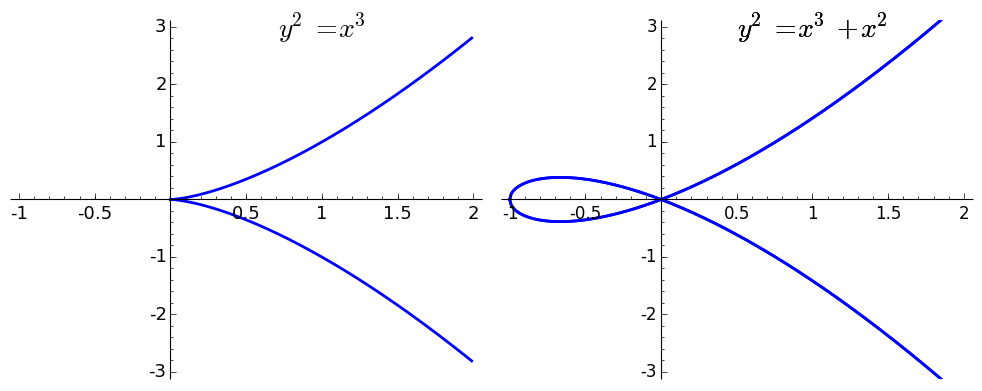
\includegraphics[width=1.0\textwidth]{graphics/singular_cubics.png}
    \caption{An example of two singular cubics over the rationals. The singular point for both curves is at the origin; for the the left curve the singular point is a {\it cusp}, and for the right curve it is a {\it node}.}
    \label{fig:singular_cubics}
\end{figure}

In the finite field setting the notion of partial derivatives still makes sense, so one may define singular points accordingly. Bad reduction at a prime may be classified into one of three types according to the nature of the tangent space at the singular point on $\tilde{E}/\Fp$.
\begin{definition}
Let $E$ have bad reduction at $p$; let $P$ be the singular point on $\tilde{E}/\Fp$, and let $T_P(E)$ be the tangent space at $P$.
\begin{itemize}
\item If the $T_P(E)$ is one-dimensional, then $P$ is a cusp, and $E$ is said to have {\it additive reduction} at $p$.
\item Otherwise $T_P(E)$ is two-dimensional, and $P$ is then a node; $E$ is then said to have {\it multiplicative reduction} at $p$. Furthermore, multiplicative reduction can be decomposed into two cases:
\begin{itemize}
\item If $T_P(E)$ is defined over $\Fp$, then $E$ is said to have {\it split multiplicative reduction} at $p$
\item Otherwise $T_P(E)$ is defined over a quadratic extension of $\Fp$, and $E$ is said to have {\it non-split multiplicative reduction} at $p$.
\end{itemize}
\end{itemize}
\end{definition}

Primes of bad reduction are packaged together into an invariant called the {\it conductor} of $E$:
\begin{definition}
The conductor of $E$, denoted by $N_E$, is a positive integer given by
\begin{equation}
N_E = \prod_{p} p^{f_p(E)},
\end{equation}
where $p$ ranges over all primes, and for $p \ne 2$ or $3$,
\begin{equation}
f_p(E) = \begin{cases} 0, & \text{$E$ has good reduction at $p$} \\ 1, & \text{$E$ has multiplicative reduction at $p$} \\ 2, & \text{$E$ has additive reduction at $p$.}\end{cases}
\end{equation}
For $p=2$ and $3$, the exponent $f_p(E)$ is still zero if $p$ is good; however the exponent may be as large as $8$ and $5$ respectively if $p$ is bad.
\end{definition}
The ``proper" definition of the conductor is Galois representation-theoretic and is defined in terms of the representation of the inertia group at $p$ on the torsion subgroup of $E$; for $p\ne 2$ or $3$ this reduces to the definition given above, but for $2$ and $3$ there may be nontrivial wild ramification which increases the exponent up to the stated amounts. A full technical definition of the conductor is given in \cite[pp. 379-396]{Sil-1994}. In any case (including $2$ and $3$), the exponent $f_p(E)$ may be computed efficiently by Tate's algorithm, as detailed in the previous section of the same book \cite[pp. 361-379]{Sil-1994}. \\

%%%%%%%%%%%%
\subsection{Elliptic curve $L$-functions}

We now move on to the definition of the $L$-function attached to an elliptic curve. For this we must define the numbers $a_p(E)$:
\begin{definition}\label{def:a_p} \mbox{}
\begin{itemize}
\item For good primes $p$ (i.e. when $p \nmid N_E$), let
\begin{equation}
a_p(E) = p+1-\#\set{\EFp},
\end{equation}
where $\#\set{\EFp}$ is the number of points on $E/\Fp$;
\item For bad primes (when $p \mid N_E$), let
\begin{equation}
a_p(E) := \begin{cases}
+1 & \text{if $E$ has split multiplicative reduction at $p$} \\
-1 & \text{if $E$ has non-split multiplicative reduction at $p$} \\
0 & \text{if $E$ has additive reduction at $p$.}
\end{cases}
\end{equation}
\end{itemize}
\end{definition}

Hasse's theorem states that the number of points on $E$ modulo $p$ can never be too far from $p+1$:
\begin{theorem}[Hasse, 1936]
For all elliptic curves $E/\QQ$ and all primes $p$,
\begin{equation}
|a_p(E)| \le 2\sqrt{p}.
\end{equation}
\end{theorem}

For ease of notation, when $E$ is fixed we will let $a_p := a_p(E)$, letting the dependence on $E$ be understood. \\

The Sato-Tate Conjecture, now a theorem thanks to Taylor, goes even further, giving an asymptotic distribution on the $a_p$:
\begin{theorem}[Taylor, 2006-]
For fixed $E/\QQ$, the set of normalized $a_p$ values $\set{\frac{a_p}{2\sqrt{p}}: p \text{ prime}}$ obey a semicircular distribution on the interval $[-1,1]$. That is, for $1\le a \le b \le 1$, the asymptotic proportion of primes for which $a \le \frac{a_p}{2\sqrt{p}} \le b$ is equal to the proportion of the area under the unit semicircle between $a$ and $b$.
\end{theorem}

\begin{definition} \mbox{}

The $L$-function attached to $E$ is a complex analytic function $L_E(s)$, defined initially on some right half-plane of the complex plane.
\begin{itemize}
\item The Euler product of the $L$-function attached to $E$ is given by
\begin{equation}
L(E,s) = \prod_{p} \frac{1}{1 - a_p p^{-s} + \epsilon(p)p^{1-2s}},
\end{equation}
where $\epsilon(p) = 0$ for bad $p$, and $1$ for good $p$.
\item The Dirichlet series for $L_E(s)$ is given by
\begin{equation}
L(E,s) = \sum_{n=1}^{\infty} a_n n^{-s}.
\end{equation}
where for composite $n$, $a_n$ is defined to be the integer coefficient of $n^{-s}$ obtained by multiplying out the Euler product for $L(E,s)$.
\end{itemize}
\end{definition}
Again, we will often write $\Les$ or just $L(s)$ to simplify notation. \\

\begin{corollary} \mbox{}
\begin{itemize}
\item Hasse's Theorem implies that the Euler product and Dirichlet series for $\Les$ converge absolutely for $\Re(s) > \frac{3}{2}$.
\item Sato-Tate implies that the Euler product and Dirichlet series for $\Les$ converge conditionally for $\Re(s) > \frac{1}{2}$.
\end{itemize}
\end{corollary}

In this work we more often use the completed $L$-function attached to $E$:
\begin{definition}
The {\it completed $L$-function} attached to $E$ is given by
\begin{equation}
\Lambda_E(s) = (N_E)^{\frac{s}{2}}(2\pi)^{-s}\Gamma(s)\Les,
\end{equation}
where $N_E$ is the conductor of $E$ and $\Gamma(s)$ the usual Gamma function on $\CC$.
\end{definition}

Thanks to the modularity theorem, we may in fact analytically continue $\Les$ and $\Lams$ to be entire functions defined on all of $\CC$.
\begin{theorem}[Breuille, Conrad, Diamond, Taylor, Wiles et al., 1995,1999,2001] \mbox{}\\
There exists an integral newform $f = \sum_n a_n q^n$ of of weight $k=2$ and level $N_E$ such that $\Les = L_f(s)$.
\end{theorem}

The modularity theorem above is essentially the converse of the theorem by Shimura in the 1960s: if $f$ is a weight $2$ newform of level $N_E$ with rational Fourier coefficients, then there exists some elliptic curve $E/\Q$ of conductor $N_E$ such that $L_f(s) = L_E(s)$. Hence any theorem about elliptic curve $L$-functions is thus really a theorem about $L$-functions of weight 2 newforms in disguise. \\

\begin{corollary} \mbox{}
\begin{itemize}
\item $\Lams$ extends to an entire function on $\CC$. Specifically, $\Lams$ obeys the {\it functional equation}
\begin{equation}
\Lams = w_E \Lambda_E(2-s),
\end{equation}
where $w_E \in \set{-1, 1}$ is the action of the Atkin-Lehner involution on the newform attached to $E$.
\item $\Les$ extends to an entire function on $\CC$ via the definition of $\Lams$ and the functional equation above.
\end{itemize}
\end{corollary}

We reproduce the analytic continuation for $\Lams$ explicitly below. Define the auxiliary function $\lambda_E(s)$ by
\begin{equation}\label{eqn:Lams_analytic_continuation}
\lambda_E(s) = \left(\frac{\sqrt{N_E}}{2\pi}\right)^{s} \sum_{n=1}^\infty a_n n^{-s}\Gamma \left(s,\frac{2\pi n}{\sqrt{N_E}}\right),
\end{equation}
where all the quantities are as defined previously, and $\Gamma(s,x)$ is the upper incomplete Gamma function on $\CC\cross \RR_{>0}$. The sum converges absolutely for any $s$, so $\lambda_E(s)$ is entire. Then
\begin{equation}
\Lambda_E(s) = \lambda_E(s) + w_E \lambda_E(2-s).
\end{equation}
Knapp goes through the proof of this formula in \cite[pp. 270-271]{Kna-1992}. \\

\begin{definition}
$E$ is said to have {\it even parity} if $w_E = 1$, and {\it odd parity} if $w_E = -1$.
\end{definition}

The functional equation for $\Lams$ shows that it is either symmetric or antisymmetric about the line $\Re(s) = 1$; moreover, since all the constituent parts for $\Lams$ are defined over the reals, $\Lams$ is also conjugate symmetric about the real axis. It follows that $\Lams$ is highly symmetric about the point $s=1$. This is formalized in the following statement:
\begin{proposition}
As a function of $s$, $\Lambda_E(1+s)$ is even if $E$ has even parity, and odd if $E$ has odd parity.
\end{proposition}
This follows immediately from the functional equation. \\

\begin{definition} For elliptic curve $L$-functions:
\begin{itemize}
\item The point $s=1$ is called the {\it central point} or the {\it critical point}.
\item The vertical line of symmetry $\Re(s)=1$ is called the {\it critical line}.
\item The vertical strip $0 \le \Re(s) \le 2$ is call the {\it critical strip}.
\end{itemize}
\end{definition}

There is an oft-quoted anecdote that the way to differentiate analytic number theorists from algebraic number theorists is that for elliptic curve $L$-functions the former normalize so that the critical line lies at $\Re(s) = \frac{1}{2}$ (as is the case with $\zeta(s)$), while the latter keep the critical line at $\Re(s)=1$. In this thesis we work mostly with $L_E(1+s)$ and $\Lambda_E(1+s)$ which shifts the critical line to the imaginary axis; a move which is bound to antagonize both parties equally! \\

A standard result with $L$-functions of Hecke eigenforms (of elliptic curve $L$-functions are a subset) is that ``all the interesting stuff happens inside the critical strip'':
\begin{proposition}
For any $E/\QQ$,
\begin{equation}
\Lambda_E(1+s) \ne 0 \;\;\mbox{when}\;\; |\Re(s)| > \frac{1}{2}.
\end{equation}
\end{proposition}
This can be proven by showing that the logarithmic derivative of $\Lambda_E(1+s)$ converges absolutely for $\Re(s) > \frac{1}{2}$; see the corollary to Proposition \ref{lem:ldLe_bound} for a proof. The statement can with a bit more work be strengthened to asserting that all zeros are {\it strictly} inside the critical strip). In fact, the Generalized Riemann Hypothesis asserts that
\begin{equation}
\Lambda_E(1+s) \ne 0  \;\;\mbox{when}\;\; \Re(s) \neq 0.
\end{equation}
From the functional equation we get that $\Les$ has simple zeros at the nonpositive integers; these are denoted the {\it trivial} zeros of $\Les$. Zeros inside the critical strip are called {\it nontrivial}. The Generalized Riemann Hypothesis (formally stated in Section \ref{sec:conjectures}) asserts that all nontrivial zeros of $\Les$ lie on the critical line $\Re(s)=1$. 

If $\Les$ has a zero at the central point, it may or may not have multiplicity greater than 1.
\begin{definition}
Let $E$ be an elliptic curve over $\Q$ and let $\Les$ be its $L$-series. The {\it analytic rank} of $E$, denoted $r_{an}(E)$ or just $r_{an}$ is the order of vanishing of $L_E(s)$ at the central point $s=1$. That is, if the Taylor series of $\Les$ about $s=1$ is
\begin{equation}
L_E(1+s) = a_0 + a_1 s + a_2 s^2 + \cdots,
\end{equation}
then $a_n = 0$ for $0 \le n < r_{an}$ and $a_{r_{an}} \ne 0$.
\end{definition}
We will work a lot with the leading coefficient of the $L$-seres at the central point, so it's worth giving it a name. To this end:
\begin{definition} \mbox{}
\begin{itemize}
\item Let $C\pr_E$ (or just $C\pr$ when $E$ is fixed) be the leading coefficient of $L_E(s)$ at the central point (the constant $a_{r_{an}}$ in the definition above).
\item Let $C_E$ (or just $C$ when $E$ is fixed) be the leading coefficient of $\Lams$ at the central point.
\end{itemize}
\end{definition}
Observe that $C\pr_E = \frac{2\pi}{\sqrt{N_E}}\cdot C_E$. We will most often work with the latter, hence the notation. \\

We may use Equation \ref{eqn:Lams_analytic_continuation} to produce formulae for the value of $\Lams$ and its higher derivatives at the central point:
\begin{proposition} \mbox{}
\begin{enumerate}
\item \begin{equation}
\Lambda_E(1) = \begin{cases} \frac{\sqrt{N_E}}{\pi} \sum_{n=1}^{\infty}\frac{a_n}{n} e^{-\frac{2\pi}{\sqrt{N_E}}\cdot n}, & w_E = 1 \\ 0, & w_E = -1 \end{cases}.
\end{equation}
\item When $m$ has the same parity as $E$, the $m$th derivative of $\Lams$ at the central point is given by
\begin{equation}\label{eqn:central_derivatives}
\Lambda_E^{(m)}(1) = 2 \sum_{n=1}^\infty a_n \int_{1}^{\infty} \left(\log \frac{t}{\sqrt{N_E}}\right)^m e^{-\frac{2\pi n}{\sqrt{N_E}}\cdot t} \; dt.
\end{equation}
When $m$ is opposite in parity to $E$, then $\Lambda_E^{(m)}(1) = 0$.
\end{enumerate}
\end{proposition}

\begin{proof}
Observe that the series in equation \ref{eqn:Lams_analytic_continuation} converges uniformly over the interval of integration; we may therefore swap the integral and summation signs. After a change of variables we get
\begin{equation*}
\lambda_E(1+s) = N_E^{\frac{1+s}{2}}  \int_{\frac{1}{\sqrt{N_E}}}^{\infty} x^s f_E(it) \; dt  = N_E^{\frac{1+s}{2}}  \sum_{n=1}^\infty a_n \int_{\frac{1}{\sqrt{N_E}}}^{\infty} t^s e^{-2\pi nt} \; dt,
\end{equation*}
where $f_E$ is the cusp form attached to $E$. Both $t^s e^{-2\pi nt}$ and its derivative w.r.t. $s$ are continuous over the integration interval for any $n$, so by the Leibniz integration rule we may differentiate under the integral sign and evaluate at $s=1$ to get
\begin{equation}\label{eqn:lambda_derivs}
\lambda_E^{(m)}(1) = \sqrt{N_E}\cdot \sum_{n=1}^\infty a_n \int_{\frac{1}{\sqrt{N_E}}}^{\infty} (\log t)^m e^{-2\pi n t} \; dt.
\end{equation}
Equation \ref{eqn:central_derivatives} follows by substituting $t \mapsto \sqrt{N_E} \cdot t$. For $m=0$ the integrals may be evaluated directly: $\int_{1}^{\infty} e^{-\frac{2\pi n t}{\sqrt{N_E}}} \; dt = \frac{\sqrt{N_E}}{2\pi n} e^{-\frac{2\pi n}{\sqrt{N_E}}}$.
\end{proof}


Equation \ref{eqn:central_derivatives} allows us to establish bounds on the coefficients of the Taylor expansion of $\Lams$ about the central point. For this we will need the following technical lemma:
\begin{lemma}\label{lem:central_deriv_int_bounds}
Let $N_E,n \in \ZZ_{>0}$, and suppose $m$ is a positive integer such that $m < \frac{1}{2}\log N_E$. Then
\begin{equation}
\left| \int_{\frac{1}{\sqrt{N_E}}}^{\infty} (\log t)^{m} e^{-2\pi n t} \; dt \right| < \frac{\left(\frac{1}{2} \log N_E\right)^{m}}{2\pi n}\left[ e^{-\frac{2\pi n}{\sqrt{N_E}}} + \frac{e^{-2\pi n\sqrt{N_E}}}{2\pi n \sqrt N_E} \right].
\end{equation}
\end{lemma}
\begin{proof}
We split the integral in two, dealing with the intervals $\frac{1}{\sqrt{N_E}}$ to $\sqrt{N_E}$ and $\sqrt{N_E}$ to $\infty$ separately. Now $(\log t)^{m}$ is at most $(\frac{1}{2}\log N_E)^m$ in magnitude on $[\frac{1}{\sqrt{N_E}},\sqrt{N_E}]$, so
\begin{equation*}
\left| \int_{\frac{1}{\sqrt{N_E}}}^{\sqrt{N_E}} (\log t)^{m} e^{-2\pi n t} \; dt \right| < \left(\frac{1}{2} \log N_E\right)^m \int_{\frac{1}{\sqrt{N_E}}}^{\sqrt{N_E}} e^{-2\pi n t} \; dt < \frac{\left(\frac{1}{2} \log N_E\right)^{m}}{2\pi n}\left(e^{-\frac{2\pi n}{\sqrt{N_E}}} - e^{-2\pi n\sqrt{N_E}}\right).
\end{equation*}
For the integral on $[\sqrt{N_E},\infty)$, we use integration by parts to get
\begin{equation*}
\int_{\sqrt{N_E}}^{\infty} \left(\log t \right)^{m} e^{-2\pi n t} \; dt = \frac{\left(\frac{1}{2} \log N_E\right)^{m}}{2\pi n}\cdot e^{-2\pi n\sqrt{N_E}} + \frac{m}{2\pi n} \int_{\sqrt{N_E}}^{\infty} \frac{\left(\log t \right)^{m-1}}{t} e^{-2\pi n t} \; dt.
\end{equation*}
If $m < \frac{1}{2}\log N_E$, then $\frac{\left(\log t \right)^{m-1}}{t}$ is decreasing for $t > \sqrt{N_E}$, so we have
\begin{equation*}
\frac{m}{2\pi n} \int_{\sqrt{N_E}}^{\infty} \frac{\left(\log t \right)^{m-1}}{t} e^{-2\pi n t} \; dt < \frac{m\left(\frac{1}{2} \log N_E\right)^{m-1}}{2\pi n\sqrt{N_E}} \int_{\sqrt{N_E}}^{\infty} e^{-2\pi n t} \; dt < \frac{\left(\frac{1}{2} \log N_E\right)^{m}}{(2\pi n)^2 \sqrt{N_E}} \cdot e^{-2\pi n \sqrt{N_E}}.
\end{equation*}
Add up all the values and you get the established result.
\end{proof}

With the above lemma in hand, we establish an upper bound on the magnitude of the $m$th Taylor coefficient of $\Lams$ at the central point.
\begin{proposition}\label{prop:central_deriv_bounds}
Let $E$ have conductor $N_E$ and completed $L$-function $\Lams$. Then so long as $m<\frac{1}{2}\log N_E$, the $m$th derivative of $\Lams$ at the central point is bounded explicitly in terms of $N_E$ and $m$ by
\begin{equation}
\left| \Lambda_E^{(m)}(1)\right| < \frac{(\frac{1}{2}\log N_E)^m}{2\pi^2}\left(N_E + \frac{1}{e^{2\pi\sqrt{N_E}}-1} \right).
\end{equation}
That is, for fixed $m$ the $m$th Taylor coefficient of $\Lams$ is $O\left( N_E(\frac{1}{2}\log N_E)^m\right)$; the second term inside the final parentheses is negligible for $N_E\gg1$.
\end{proposition}

\begin{proof}
From Lemma \ref{lem:central_deriv_int_bounds} and Equation \ref{eqn:lambda_derivs} we have that
\begin{equation*}
\left| \Lambda_E^{(m)}(1)\right| < 2 \sqrt{N_E} \sum_{n=1}^{\infty} |a_n| \cdot \left[\frac{\left(\frac{1}{2} \log N_E\right)^{m}}{2\pi n}\left( e^{-\frac{2\pi n}{\sqrt{N_E}}} + \frac{e^{-2\pi n\sqrt{N_E}}}{2\pi n \sqrt N_E} \right)\right].
\end{equation*}
Using the bound $|a_n(E)| \le n$ for any $E$, we get
\begin{equation*}
\left| \Lambda_E^{(m)}(1)\right| < \frac{ \sqrt{N_E}\left(\frac{1}{2} \log N_E\right)^{m}}{\pi} \sum_{n=1}^{\infty} e^{-\frac{2\pi n}{\sqrt{N_E}}} + \frac{\left(\frac{1}{2} \log N_E\right)^{m}}{2\pi^2} \sum_{n=1}^{\infty} \frac{e^{-2\pi n\sqrt{N_E}}}{n}.
\end{equation*}
Now
\begin{equation*}
\sum_{n=1}^{\infty} e^{-\frac{2\pi n}{\sqrt{N_E}}} = \frac{1}{e^{\frac{2\pi n}{\sqrt{N_E}}}-1}< \frac{\sqrt{N_E}}{2\pi},
\end{equation*}
while $\sum_{n=1}^{\infty} \frac{e^{-2\pi n\sqrt{N_E}}}{n} \le \sum_{n=1}^{\infty} e^{-2\pi n\sqrt{N_E}} = \frac{1}{e^{2\pi\sqrt{N_E}}-1}$.
\end{proof}

Note that for fixed $N_E$, if we allow $m \to \infty$, we actually have that the $m$th derivative can grow like $O\left(\frac{m!!}{(2\pi e)^{m/2}}\right)$, where $m!! = m(m-2)\cdots$ is the double factorial on $m$ i.e. faster than exponentially in $m$. However, this behavior only starts to show when $m\gg\log N_E$ -- hence our restriction on the magnitude of $m$. This will in practice never be an issue: we are primarily interested in the central derivatives in order to establish results about the analytic rank of $E$. Since maximum analytic rank grows more slowly than $\log N_E$ (c.f. Corollary \ref{cor:logderiv_rank_bound}), we will never need to consider $\Lambda_E^{(m)}(1)$ for $m> \frac{1}{2}\log N_E$. \\


Crucial to this thesis, $L_E(s)$ and its derivatives can be provably computed to a given precision in time that scales with the square root of the conductor of $E$:
\begin{proposition}\label{prop:L_E_time_complexity}
When $m<\frac{1}{2} \log N_E$, the $m$th derivative of $L_E(s)$ at the central point can be provably computed to $k$ bits precision in $\softO(k\cdot \sqrt{N_E})$ time, where $N_E$ is the conductor of $E$.
\end{proposition}
This is proven in full in the PhD thesis of Robert Bradshaw \cite{Bra-2010}. The basic argument is as follows:
\begin{enumerate}
\item Since the two differ by an exponential and a Gamma factor, computing $L_E^{(m)}(1)$ takes the same order of magnitude time as computing $\Lambda_E^{(m)}(1)$. This may be achieved, for example, by the formula given in Equation \ref{eqn:central_derivatives};
\item The integral $\int_{1}^{\infty} \left(\log \frac{t}{\sqrt{N_E}}\right)^m e^{-\frac{2\pi n}{\sqrt{N_E}}\cdot t} \; dx$ can be computed to $k$ bits precision in time that scales proportional to $k$, is independant of $n$ and subpolynomial in $N_E$;
\item The number of terms needed in the sum to achieve $k$ bits precision is $O\left( \log(N_E)^m\sqrt{N_E}\right)$;
\item Computing $a_n$ can be done in time polynomial in $\log n$;
\item Combining the above, computation time is dominated by evaluating $O( \log(N_E)^m\sqrt{N_E})$ integrals and $a_n$ values. That is, the sum can be evaluated to $k$ bits precision in time scaling with $k \sqrt{N_E}$ times some power of $\log N_E$.
\end{enumerate}
We will use the result of Proposition \ref{prop:L_E_time_complexity} directly in the proof of Theorem \ref{thm:main_theorem}. In fact, the $\softO(\sqrt{N_E})$ time needed to evaluate central derivatives of $\Les$ is the computational bottleneck in algorithm \ref{algo:compute_rank}; all other steps scale in time subpolynomial in $N_E$. 


\newpage
%%%%%%%%%%%%%%%%%%%%%%%%%%
\section{The Three Big Conjectures}\label{sec:conjectures}

The main results in this thesis are contingent on the Birch and Swinnerton-Dyer conjecture, The Generalized Riemann Hypothesis and the ABC conjecture. We reproduce the three conjectures in full below; citations for the papers in which they first appeared or are fully formulated are listed at the top of each conjecture. \\

The Birch and Swinnerton-Dyer conjecture (BSD) is needed to establish a way to compute and hence bound the magnitude of the leading coefficient of $\Les$ at the central point.
\begin{conjecture}[Birch, Swinnerton-Dyer]\label{conj:BSD} \cite{BSD-1965}
\mbox{}
\begin{enumerate}
\item $r_{an} = r$; that is, the analytic rank of $E$ is equal to its algebraic rank.
\item The leading coefficient at the central point in $L_E(s)$ is given by
\begin{equation}\label{eqn:BSD_formula}
C\pr_E = \left(\frac{\Omega_E\cdot\Reg_E\cdot\#\Sha(E/\Q)\cdot\prod_p c_p}{(\#E_{\text{Tor}}(\Q))^2}\right),\end{equation}
where
\begin{itemize}
\item $r$ is the algebraic rank of $E(\Q)$,
\item $\Omega_E$ is the real period of (an optimal model of) $E$,
\item $\Reg_E$ is the regulator of $E$,
\item $\#\Sha(E/\Q)$ is the order of the Shafarevich-Tate group attached to $E/\Q$,
\item $\prod_p c_p$ is the product of the Tamagawa numbers of $E$, and
\item $\#E_{\text{Tor}}(\Q)$ is the number of rational torsion points on $E$.
\end{itemize}
\end{enumerate}
\end{conjecture}

For an excellent description of the conjecture and a breakdown of the arithmetic invariants mentioned above, see Andrew Wiles' official description of the BSD Conjecture on the Clay Math website \cite{Wil-BSD}. \\

The Generalized Riemann Hypothesis (GRH), as the name suggests, generalizes the famous conjecture first posed by Bernhard Riemann in 1859 \cite{Rie-1859}. The (standard) Riemann Hypothesis asserts that all nontrivial zeros of the Riemann zeta function $\zeta(s)$ occur on the vertical line $\Re(s)=\frac{1}{2}$. It is hard to track down where the Generalized Riemann Hypothesis was first formulated in its full generality (Conrey gives a good exposition in \cite{Con-2003}), but it asserts that for a large class of suitably defined $L$-functions, the nontrivial nonreal zeros will occur on a single vertical line in the complex plane (where the exact lateral placement of said line depends on the class of $L$-function being considered). We use GRH as it applies to elliptic curve $L$-functions:
\begin{conjecture}[Generalized Riemann Hypothesis for Elliptic Curves, version 1] \cite{Rie-1859} \cite{Con-2003}
\label{conj:GRH1}
\mbox{}
Let $E$ be an elliptic curve over $\Q$, and let $\Les$ be its $L$-series. If $\rho$ is a nontrivial zero of $\Les$ with nonzero imaginary part, then $\Re(\rho) = 1$.
\end{conjecture}
That is, $\Les$ is never zero outside of the {\it critical line} $\Re(s)=1$ and the nonpositive integers. There are numerous equivalent formulations of GRH; we will most often use the following pertaining to the shifted completed $L$-function:
\begin{conjecture}[Generalized Riemann Hypothesis for Elliptic Curves, version 2] \cite{Rie-1859} \cite{Con-2003}
\label{conj:GRH2}
 \mbox{}
 Let $E$ be an elliptic curve over $\Q$, and let $\Lams$ be the completed $L$-function attached to $E$. Then
\begin{enumerate}
\item $\Lambda_E(1+s) = 0 \Longrightarrow \Re(s) = 0$.
\end{enumerate}
\end{conjecture}

Finally, we will need strong form of the ABC conjecture of Masser and Oesterl\'{e} in order to establish lower bounds on the regulator and real period of $E$.
\begin{conjecture}[Masser-Oesterl\'{e}] \cite{Mas-1985} \cite{Oes-1988}
\label{conj:ABC} \\
Let $(a,b,c)$ be a triple of coprime positive integers such that $a+b = c$, and let $\rad(abc) = \prod_{p | abc} p$ be the product of all primes dividing $a$, $b$ and $c$. Then for any $\epsilon > 0$ there is a constant $K_{\epsilon}$ such that
\begin{equation}
c < K_{\epsilon}\rad(abc)^{1+\epsilon}.
\end{equation}
\end{conjecture}

The ABC conjecture is famous for the large number of other results that it implies. Of these, we will need two that relate to elliptic curves. It is a relatively straightforward exercise to show that the conductor of an elliptic curve divides its minimal discriminant. Szpiro's conjecture, formulated in the 1980s, asserts that the latter cannot be too big in terms of the former:
\begin{conjecture}[Szpiro] \cite{szp-1987}
\label{conj:Szpiro} \\
Let $E$ be an elliptic curve over $\QQ$ with conductor $N_E$ and minimal discriminant $D_E$. Then for any $\epsilon > 0$ there is a constant $K_{\epsilon}$ such that
\begin{equation}
|D_E| < K_{\epsilon}\cdot (N_E)^{6+\epsilon}.
\end{equation}
\end{conjecture}

We will also invoke a equivalent version of the above conjecture:
\begin{conjecture}[Modified Szpiro]\label{conj:modified_szpiro}
Let $c_4$ and $c_6$ be the $c$-invariants of a minimal model of $E/\QQ$, as defined in Section \ref{subsec:notation}. Then for any $\epsilon>0$ there is a constant $K_{\epsilon}$ independent of $E$ such that
\begin{equation}
\max\set{|c_4|^3,|c_6|^2} \le K_{\epsilon}\cdot (N_E)^{6+\epsilon}.
\end{equation}
\end{conjecture}

Lang's conjecture posits that the height of a point on a rational curve cannot be too small in terms of the discriminant:
\begin{conjecture}[Lang] \cite[pp. 73-74]{Lang-1997}
\label{conj:Lang} \\
There is a positive constant $M_0$ such that for any elliptic curve $E/\QQ$ with minimal discriminant $D_E$, the N\'{e}ron-Tate canonical height of any nontorsion point $P\in E(\QQ)$ obeys
\begin{equation}
\hat{h}(P) \ge M_0\log |D_E|.
\end{equation}
\end{conjecture}

%\begin{conjecture}[Hall]\label{conj:Hall}
%For any $\epsilon > 0$ there is a constant $K_{\epsilon}$ such that for any $x,y \in \ZZ$ such that $x^3-y^2 \ne 0$, we have
%\begin{equation}
%|x^3-y^2| \ge K_{\epsilon}\cdot |x|^{\frac{1}{2}-\epsilon}.
%\end{equation}
%That is, if $x^3-y^2 \ne 0$, then it cannot be much smaller in magnitude than about $\sqrt{|x|}$.
%\end{conjecture}


% ========== Chapter 4
\chapter{An Algorithm to Compute Rank}\label{chap:main_theorem}
% ----- CHAPTER 4: AN ALGORITHM TO COMPUTE RANK ----- %

%%%%%%%%%%%%%%%%%%%%%%%%%%%
\section{Proof of the Main Theorem}\label{sec:main_thrm_proof}

In this section we prove Theorem \ref{thm:main_theorem}: specifically, that Algorithm \ref{algo:compute_rank} is guaranteed, assuming BSD and ABC and optionally GRH, to correctly output an elliptic curve's rank in time $\softO(\sqrt{N_E})$, where $N_E$ is the conductor of the input curve. Note that the proof will quote certain results established later in this work. \\

\begin{proposition}\label{prop:k_bits_for_leading_coeff}
Let $E$ have $L$-function $\Les$, conductor $N_E$ and real period $\Omega_E$, and let
\begin{equation}\label{eqn:num_bits_without_GRH}
k = 65 + 10.5 \log_2 N_E - \log_2 \Omega_E
\end{equation}
Assuming BSD and ABC, we have the following:
\begin{itemize}
\item $k = O((\log N_E)^m)$ for some $m$
\item If $L_E^{(m)}(1)=0$ for all $0 \le m < n$ and $\frac{L_E^{(n)}(1)}{n!}$ is zero to $k$ bits precision, then $L_E^{(n)}(1)$ is identically zero.
\end{itemize}
\end{proposition}
If one further assumes GRH, we may instead let
\begin{equation}\label{eqn:num_bits_with_GRH}
k = 31 + 6.7 \log_2 N_E - \log_2 \Omega_E
\end{equation}
for the same results to hold.
\begin{proof}
The first statement follows immediately from Theorem \ref{thm:real_period_lower_bound}, which states that $\Omega_E$ is bounded away from zero by a negative power of $N_E$. To prove the second statement, observe that by BSD the leading non-zero Taylor coefficient of $\Les$ at the central point is given by Equation \ref{eqn:BSD_formula}. We thus have that
\begin{equation}
C_E\pr \ge \frac{1}{256} \cdot  \Reg_E \cdot\, \Omega_E
\end{equation}
since $\prod_p c_p \ge 1$, $\# \Sha_E \ge 1$, and by Mazur's Theorem $\# E_{\text{Tor}} \le 16$. Thus
\begin{equation}
\log_2 C_E\pr \ge -16 + \log_2 \Reg_E + \log_2 \Omega_E
\end{equation}
Now by Theorem \ref{thm:regulator_lower_bound} we have that $\Reg_E\ge 2.59 \times 10^{-15} (N_E)^{-10.49}$. Thus 
$\log_2 \Reg_E \ge -48.46 - 10.49 \log_2 N_E$. We therefore have that
\begin{equation}
\log_2 C_E\pr \ge -64.46 - 10.49 \log_2 N_E + \log_2 \Omega_E > -k
\end{equation}
where $k$ is as defined above. Hence if the $n$th taylor coefficient of $\Les$ at the central point is zero to $k$ bits precision and all preceding Taylor coefficients are zero, then it {\it cannot} be the leading BSD coefficient, and so must be identically zero.

If one further assumes GRH, we instead have the bound $\Reg_E \ge 3.48 \times 10^{-5} \cdot (N_E)^{-6.70}$. Repeat as before to obtain the required precision stated in Equation \ref{eqn:num_bits_with_GRH}.
\end{proof}

Note that the $-16$ appearing in the right hand side of the above inequalities comes from bounding the order of the torsion group of $E$; this constant can therefore be reduced or eliminated by computing the torsion order of $E$ explicitly, which is quick to do. This is something that therefore should be done in any optimized implementation of Algorithm \ref{algo:compute_rank}. \\

In other words, the leading Taylor coefficient of $\Les$ at $s=1$ must be greater than $2^{-k}$ in magnitude. We now prove Theorem \ref{thm:main_theorem}: that, assuming BSD and ABC and optionally GRH, Algorithm \ref{algo:compute_rank} computes the rank of an elliptic curve in $\softO\left(\sqrt{N_E}\right)$ time.
\begin{proof}
Let $k$ be as defined according to either Equation \ref{eqn:num_bits_without_GRH} or \ref{eqn:num_bits_with_GRH} depending on whether GRH is assumed or not. That the algorithm terminates with correct output is a direct corollary from Proposition \ref{prop:k_bits_for_leading_coeff}: if $\frac{L_E^{(r)}}{r!}$ is computed to $k$ bits precision and some of those bits are nonzero {\it and} all preceding Taylor coefficients have been shown to be zero, then $r$ must be the rank of $E$; hence the output of rank$=r$ is correct. \\

In terms of time complexity, observe that $k$ is $O(\log N_E)$ in magnitude, and by Corollary \ref{cor:real_period_time_complexity}, can be computed in time polynomial in $\log N_E$. By Corollary \ref{cor:better_an_bound}, we need to evaluate at most $\frac{1}{2}\log N_E +1.6$ central Taylor coefficients of $\Les$ to $k$ bits precision; Proposition \ref{prop:L_E_time_complexity} states that each of these can be done in $\softO\left(k\cdot \sqrt{N_E}\right)$ time. Hence the algorithm is guaranteed to terminate in time at most 
\begin{equation}
O(\log N_E) + \left(\frac{1}{2}\log N_E + 1.6\right) \cdot \softO\left(k\cdot \sqrt{N_E}\right) = \softO\left(\sqrt{N_E}\right)
\end{equation}
since $k$ is sub-polynomial in $N_E$. The $\frac{1}{2}\log N_E + 1.6$ in the above statements may be replaced with $0.32\log N_E + 0.5$ if GRH is assumed, but resulting time complexity remains $\softO\left(\sqrt{N_E}\right)$.
\end{proof}


\newpage
%%%%%%%%%%%%%%%%%%%%%%%%%%%
\section{The Real Period}

The real period of a rational elliptic curve $E$ is a measure of the ``size'' of the set of {\it real} points on $E$. \\

Recall that $E(\CC)$, the group of complex points on $E$, is isomorphic via the (inverse of the) Weierstrass $\wp$-function to $\CC$ modulo a lattice under addition; that is, $E(\CC) \simeq \CC/\Lambda$, where $\Lambda = \ZZ\omega_1 + \ZZ\omega_2$, and $\omega_1,\omega_2 \in \CC$.
If $E$ is defined over the real numbers (as rational elliptic curves are), then we may always write $\omega_1$ as being positive real. The second generator $\omega_2$ can be written as being positive imaginary when $E$ has positive discriminant, or in the upper half plane with real part $\frac{\omega_1}{2}$ when $E$ has negative discriminant. [Note: some texts normalize $\omega_2$ to have imaginary part equal to $-\frac{\omega_1}{2}$ when $D_E<0$, as this sometimes makes the presentation more natural. However, for the work below we will always assume that $\Re(\frac{\omega_2}{\omega_1}) = 0$ or $\frac{1}{2}$.]

\begin{definition}\label{defn:real_period}
Let $E/\QQ$ have discriminant $D_E$, and $E(\CC) \simeq \CC/\Lambda$, where $\Lambda = \ZZ\omega_1 + \ZZ\omega_2$ and $\omega_1 \in \RR$. The {\it real period} of $E$ is defined to be
\begin{equation}
\Omega_E = \begin{cases} 2\omega_1 & D_E > 0 \\ \omega_1 & D_E < 0 \end{cases}
\end{equation}
\end{definition}

We are interested in answering the question: For a curve of a given discriminant, how big and how small can $\Omega_0$ be? Can the real period be arbitrarily small or large, or does it scale in some meaningful way with the discriminant? For our purposes, establishing a lower bound on $\Omega_E$ is what is needed to bound the central leading Taylor coefficient of $\Les$ from below. However, we include the result giving an upper bound on $\Omega_E$, as we find its implication -- that $\Omega_E$ goes to zero as $N_E$ goes to infinity -- an interesting one. \\

First, an upper bound. To this end, we have the following result from the complex theory of elliptic curves:
\begin{proposition}
Let $\Delta(z)$ be the Ramanujan Delta function on the complex upper half plane, i.e.
\begin{equation}
\Delta(z) = q \prod_{n=1}^{\infty} (1-q^n)^{24}
\end{equation}
where $q = e^{2\pi i z}$. Let $E/\CC$ have discriminant $D_E$ and lattice basis $(\omega_1,\omega_2)$ as defined above. Set $z = \frac{\omega_1}{\omega_2}$ (such that $\Im(z) > 0$). Then
\begin{equation}\label{eqn:modular_discriminant}
D = \left(\frac{2\pi}{\omega_1}\right)^{12} \Delta\left(z \right)
\end{equation}
\end{proposition}
A good treatment of elliptic and modular functions, including a proof of the above, can be found in \cite{Sil-1994}. Using this result we can readily establish an upper bound on $\Omega_E$:
\begin{proposition}\label{prop:real_period_upper_bound_discriminant}
Let $E/\QQ$ have discriminant $D_E$ and real period $\Omega_E$. Then
\begin{equation}\label{eqn:real_period_upper_bound_discriminant}
\Omega_E < 8.82921517\ldots \cdot (D_E)^{-\frac{1}{12}}
\end{equation}
\end{proposition}
\begin{proof}
Equation \ref{eqn:modular_discriminant} yields
\begin{equation}
\omega_1 = 2\pi |D_E|^{-\frac{1}{12}} \left| \Delta\left(\frac{\omega_2}{\omega_1}\right)\right|^{\frac{1}{12}}
\end{equation}
Since $E$ is defined over $\QQ$, $z = \frac{\omega_2}{\omega_1}$ has real part either equal to zero (if $D_0>0$) or equal to $\frac{1}{2}$ (if $D_E<0$). Thus $D_E>0$ corresponds to $q = e^{2\pi i z}$ being positive real lying in the open interval $(0,1)$, while $D_E<0$ corresponds to $q \in (-1,0)$. Now $\Delta$ is a cuspidal modular form on $\SL_2(\ZZ)$, so $\Delta(q)$ is continuous on $(-1,1)$ and decays to zero at $q=-1$ and $q=1$. It must therefore achieve a maximum magnitude on $(-1,0)$ and $(0,1)$. \\

The critical points of $\Delta$ have been studied in there own right -- see for example \cite{IJA-2013} and \cite{WoYo-2013}. We see that $\Delta(q)$ has precisely one critical point on each of the intervals $(-1,0)$ and $(0,1)$; these occur at $q = 0.03727681\ldots$ and $q =-0.43929305\ldots$ respectively (corresponding to $z=0.52352170\ldots i$ and $z=\frac{1}{2}+0.13091903\ldots i$ respectively). At these two values we have $|\Delta(q)|^{\frac{1}{12}}$ equal to $0.70258935\ldots$ and $1.40521323\ldots$ respectively. We conclude that
\begin{equation}
\Omega_E \le 2\pi\cdot 1.40521323\ldots \cdot  |D_E|^{-\frac{1}{12}} = 8.82921517\ldots \cdot |D_E|^{-\frac{1}{12}}
\end{equation} 
\end{proof}

Note that the real period is {\it not} invariant under isomorphism over $\QQ$. As the elliptic discriminant $D_E$ varies by a twelfth power of an integer as one considers $\QQ$-isomorphic models of $E$, the real period varies by the negative first power of that same integer. This is an immediate consequence of the following statement:
\begin{lemma}
Let $E$ be the global minimal model of a rational elliptic curve, and let $D_E$ and $\Omega_E$ be its discriminant and real period respectively. Let $E\pr$ be isomorphic to $E$ over $\QQbar$, and let $D_{E^{\pr}}$ and $\Omega_{E^{\pr}}$ be defined analogously. Then there exists a $u$ such that  $u^{12}\in \ZZ$, where $D_{E^{\pr}}=u^{12} D_E$ and $\Omega_{E^{\pr}}=\frac{1}{u}\Omega_E$.
\end{lemma}
A proof of the result regarding the discriminant can be found on pages 48-49 of \cite{Sil-1985}; the result regarding the real period follows, for example, from Equation \ref{eqn:modular_discriminant} by chasing through how $D_E$ and $\Omega$ vary under $\CC$-isomorphism. \\

Another consequence is that the bound given in Equation \ref{eqn:real_period_upper_bound_discriminant} is optimal, in the sense that the $\frac{1}{12}$ in the negative power of the the discriminant cannot be replaced with any larger value. As an explicit example, consider the family of CM elliptic curves given by Weierstrass equations
\begin{equation}
E^d: \;\; y^2 = x^3 - d^2 x
\end{equation}
for $d \in\ZZ$ positive squarefree (this is just the family of curves related to the congruent number problem, one of the oldest open problems in mathematics. For an excellent treatment on congruent numbers and how they relate to elliptic curves, see \cite{Kob-2012}). Then $E^{d}$ is just the quadratic twist by $d$ (hence the notation) of the curve
\begin{equation}
E: \;\; y^2 = x^3-x
\end{equation}
which has discriminant 64 and conductor 32. For this family we may actually write down $\Omega_{E^d}$ in terms of a special value of the Gamma function:
\begin{equation}
\Omega_{E^d} = \frac{\Gamma(\frac{1}{4})^2}{\sqrt{2\pi d}}
\end{equation}
This follows from the fact that $\frac{\omega_2}{\omega_1} = i$ for any of the $E^d$, and that
\begin{equation}
\Delta(i) = \frac{\Gamma(\frac{1}{4})^{24}}{2^{24}\pi^{18}}
\end{equation}
(first shown by Ramanujan in his second notebook -- see \cite{BeZh-1992}). Furthermore, $E^{d}$ has discriminant $D_{E^{d}} = (2d)^6$. So using equation \ref{eqn:modular_discriminant}, for congruent number curves we obtain
\begin{equation}
\Omega_{E^d} = \frac{\Gamma(\frac{1}{4})^2}{\sqrt{\pi}} \cdot (D_{E^d})^{-\frac{1}{12}} = 7.416\ldots \cdot (D_{E^d})^{-\frac{1}{12}}
\end{equation}
Since $4\pi = 12.566\ldots$ this result conforms with the bound given in Equation \ref{eqn:real_period_upper_bound_discriminant}. It should also be clear from the example above that any family of quadratic twists of a given curve will have the real period scale with the $-\frac{1}{12}$th power of the discriminant. Furthermore, since the $j$-invariant is surjective, we can find $E/\QQ$ with $z=j^{-1}(E)$ arbitrarily close to $\frac{1}{2}+0.13091903\ldots i$, so the constant $8.82921517\ldots$ obtained in Proposition \ref{prop:real_period_upper_bound_discriminant} is also optimal. \\

\begin{corollary}
For $E/\QQ$ with real period $\Omega_E$ and conductor $N_E$,
\begin{equation}
\Omega_E < 8.82921517\ldots \cdot (N_E)^{-\frac{1}{12}}
\end{equation}
That is, the real period goes to zero as the conductor of the curve goes to infinity.
\end{corollary}
This follows immediately from Proposition \ref{prop:real_period_upper_bound_discriminant}, as the conductor of an elliptic curve always divides its discriminant. Again, by the same reasoning as before this bound should be optimal. \\

Equation \ref{eqn:modular_discriminant} fives us a way to compute the real period of $E$, but it is in general not the most efficient means of doing so (as $z = \frac{\omega_1}{\omega_2}$ must be found by, for example, inverting the $j$-invariant of $E$). Instead, $\omega_1$ may be computed using the (real version of the) Gauss arithmetic-geometric mean. Recall the definition thereof: let $a,b \in \RR_{\ge0}$. Set $a_0 = a$ and $b_0 = b$, and for $n\ge 0$ let $a_{n+1} = \frac{1}{2}(a_{n}+b_{n})$ and $b_{n+1} = \sqrt{a_{n}b_{n}}$. Then $\AGM(a,b)$ is defined to be the common limit of both the $a_n$ and the $b_n$. We omit the proof that both sequences converge to the same value, but convergence is quadratic (i.e. extremely quick).

\begin{proposition}\label{prop:real_period_by_AGM}
Let $E/\Q$ have minimal Weierstrass equation $y^2 + a_1 xy + a_3 y^2 = x^3 + a_2 x^2 + a_4 x + a_6$. Write the equation in the form
\begin{equation}\label{eqn:weierstrass_with_bn}
\left(y + \frac{a_1x + a_3}{2}\right)^2 = x^3 + \frac{b_2}{4} x^2 + \frac{b_4}{2} x + \frac{b_6}{4} = (x-e_1)(x-e_2)(x-e_3)
\end{equation}
where $e_1,e_2,e_3$ are the 3 complex roots of the polynomial in $x$ on the right hand side, and $b_2$, $b_4$ and $b_6$ are as defined at the beginning of section \ref{sec:defs_background}.
\begin{enumerate}
\item If $D_E > 0$, then $e_1,e_2,e_3 \in \RR$, so without loss of generality we may order them as $e_3 > e_2 > e_1$. Then
\begin{equation}\label{eqn:omega_D_pos}
\omega_1 = \frac{\pi}{\AGM(\sqrt{e_3-e_1},\sqrt{e_3-e_2})}
\end{equation}
\item If $D_E < 0$, then the RHS polynomial has only one real root; we may write $e_3 \in \RR$ and $e_1 = \conj{e_2}$. Let $z = \sqrt{e_3-e_1} = s + it$; choose the root such that $s>0$. Then
\begin{equation}\label{eqn:omega_D_neg}
\omega_1 = \frac{\pi}{\AGM(|z|,s)}
\end{equation}
\end{enumerate}
\end{proposition}
\begin{proof}
Cremona and Cremona-Thongjunthug give good explanations and derivations this formula in \cite{Cre-1997} and \cite{Cre-2013} respectively.
\end{proof}

To get a lower bound on $\Omega_E$ from the above definitions, we will need the following technical result.
\begin{definition}
For a given $E/\QQ$, let 
\begin{equation}
d(E) = \max\set{|e_i - e_j|: \; e_i,e_j \text{ are roots of }4x^3 + b_2  x^2 + 2 b_4 x + b_6, i\ne j}
\end{equation}
be the maximum root separation of the cubic polynomial on the RHS of equation \ref{eqn:weierstrass_with_bn}
(i.e. $b_2, b_4$ and $b_6$ are the $b$-invariants of $E$).
\end{definition}
Observe that for both the positive and negative discriminant cases, the AGM in the denominators in equations \ref{eqn:omega_D_pos} and \ref{eqn:omega_D_neg} is at most $\sqrt{d(E)}$. It is useful therefore to have a bound on the magnitude of $d(E)$ in terms of the $b$-invariants:
\begin{lemma}\label{lem:root_separation_bound}
Given the above setup,
\begin{equation}
d(E) < 2+\frac{1}{2}\max\set{|b_2|,2|b_4|,|b_6|}
\end{equation}
\end{lemma}
\begin{proof}
We apply Rouche's Theorem on the polynomial $x^3 + \frac{b_2}{4} x^2 + \frac{b_4}{2} x + \frac{b_6}{4}$. Observe that $|\frac{b_2}{4} x^2 + \frac{b_4}{2} x + \frac{b_6}{4}| < |x^3|$ when $|x| < 1+\max\set{\frac{|b_2|}{4},\frac{|b_4|}{2},\frac{|b_6|}{4}}$, so by Rouche's Theorem we must have that any root $e$ of the cubic obeys $|e| <  1+\frac{1}{4}\max\set{|b_2|,2|b_4|,|b_6|}$. The result follows.
\end{proof}

\begin{corollary}\label{cor:real_period_time_complexity}
Assuming ABC, the real period of an elliptic curve can be computed to a specified precision in polynomial time and space in the number of bits of the curve's conductor.
\end{corollary}
\begin{proof}
We see from Proposition \ref{prop:real_period_by_AGM} that $\Omega_0$ can be computed by a) finding the roots of a cubic polynomial related to the Weierstrass equation for $E$, and then b) applying the AGM to a certain simple function of that cubic's roots. \\

Step a) can be achieved in polynomial time in log of the maximum magnitude of the $a$-invariants, which means it can be done in polynomial time in the $c$-invariants. By Modified Szpiro (Conjecture \ref{conj:modified_szpiro}) the conductor of a curve is bounded in magnitude by a polynomial in the $c$-invariants; chaining this all together gives us that step a) can be commuted in time polynomial in $\log N_E$, i.e. sub-polynomial in $N_E$. \\

In step b), Lemma \ref{lem:root_separation_bound} implies that the inputs to the AGM are bounded by a polynomial of the $b$-invariants of $E$, so again by Szpiro they are bounded by a power of $N_E$. The AGM converges quadratically when both the inputs are positive real; therefore it will converge to specified precision with time bounded by a polynomial of $\log N_E$. Thus altogether we see that the real period can be computed to a given precision with time polynomial in $\log N_E$, i.e. sub-polynomial in $N_E$ itself.
\end{proof}

The take-away from the above result is that computing the real period is quick, and will never be the computational bottleneck when it comes to running Algorithm \ref{algo:compute_rank}. \\

\begin{corollary}[S.]\label{ineq:Omega_bn_bound}
Let $E/\Q$ have (not necessarily minimal) Weierstrass equation \\
$y^2 + a_1 xy + a_3 y^2 = x^3 + a_2 x^2 + a_4 x + a_6$ have real period $\Omega_E$, and define $b_2$, $b_4$ and $b_6$ as at the beginning of section \ref{sec:defs_background}. Then
\begin{equation}
\Omega_E > \frac{\alpha \pi}{\sqrt{1+\frac{1}{4}\max\set{|b_2|,2|b_4|,|b_6|}}},
\end{equation}
where $\alpha = 1$ if $E$ has positive discriminant and $\frac{1}{2}$ if $E$ has negative discriminant.
\end{corollary}
\begin{proof}
This follows immediately from the definition of $\Omega_E$ given in Proposition \ref{prop:real_period_by_AGM} and Lemma \ref{lem:root_separation_bound}.
\end{proof}

Again, this bound is optimal in the sense that the square root sign in the denominator cannot be replaced with any smaller exponent. To see this, consider the family of elliptic curves
\begin{equation}
E_n: \;\; y^2 = x^3 - (nx-1)^2.
\end{equation}
For a given $n$, $E_n$ has $b_2,b_4$ and $b_6$ equal to $-4n^2,4n$ and $-4$ respectively.

The polynomial $x^3 + \frac{b_2}{4} x^2 + \frac{b_4}{2} x + \frac{b_6}{4} = x^3 -n^2 x^2 + 2n x - 1$ has a single root at $n^2 - O(\frac{1}{n})$ and two roots very close to the origin with magnitude $O(\frac{1}{n})$. Hence the real period for $E_n$ is
\begin{equation}
\Omega_{E_n} = \frac{2\pi}{n} + O\left(\frac{1}{n}\right).
\end{equation}

On the other hand, for a given $n$
\begin{equation}
1+\frac{1}{4}\max\set{|b_2|,2|b_4|,|b_6|} = 1+n^2.
\end{equation}
for $n\ge 2$. So for this family of curves the lower bound given by inequality \ref{ineq:Omega_bn_bound} is $\frac{\pi}{\sqrt{1+n^2}}$. Since $\Omega_{E_n}$ asymptotes to twice this value, it is clear that the bound would be violated for sufficiently large $n$ if the square root were replaced with a smaller power. \\

Finally, if we assume the Szpiro conjecture, Corollary \ref{ineq:Omega_bn_bound} allows us to the real period of a minimal model of $E$ from below in terms of that curve's conductor. We will invoke a slight reformulation of Modified Szpiro (Conjecture \ref{conj:modified_szpiro}): Suppose the minimal short Weierstrass model of $E$ is $y^2 = x^3+Ax+B$, i.e. there does not exist any prime $p$ such that $p^4|A$ and $p^6|B$. Then for any $\epsilon>0$ there is a constant $K(\epsilon)$ independent of $E$ such that
\begin{equation}
\max\set{|A|^3,|B|^2} \le K(\epsilon)\cdot (N_E)^{6+\epsilon}
\end{equation}
(Since for a curve in short Weierstrass form $c_4 = -48A$ and $c_6=-864B$, we see that the above statement and Modified Szpiro are equivalent). Using this, we obtain the following:
\begin{theorem}\label{thm:real_period_lower_bound}
Let $E$ have conductor $N_E$, and let $\Omega_E$ be the real period of a minimal model of $E$. Then, assuming ABC, for any $\epsilon>0$ there is a constant $K(\epsilon)$ independent of $E$ such that 
\begin{equation}
\Omega_E > K(\epsilon) \cdot (N_E)^{-\frac{3}{2}-\epsilon}
\end{equation}
\end{theorem}
\begin{proof}
Let $E$ be given by its minimal short Weierstrass equation $y^2 = x^3+Ax+B$. $E$ then has $b$-invariants $b_2=0$, $b_4 = 2A$ and $b_6 = 4B$, so by Lemma \ref{ineq:Omega_bn_bound} the real period of $E$ obeys
\begin{equation}\label{eqn:Omega_bound_short_weierstrass}
\Omega_E > \frac{\pi}{2\sqrt{1+\max\set{|A|,|B|}}}
\end{equation}
Now by the aforementioned version of Szpiro, for any $\epsilon>0$ we have
\begin{align*}
\sqrt{1+\max\set{|A|,|B|}} &<  1 + \max\set{|A|^2,|B|^2}^\frac{1}{4} \\
&\le 1 + \max\set{|A|^3,|B|^2}^\frac{1}{4} \quad\quad\mbox{since $A \in \ZZ$} \\
&\le 1 +\left[K(\epsilon) (N_E)^{6+\epsilon} \right]^\frac{1}{4} \\
\Longrightarrow \sqrt{1+\max\set{|A|,|B|}} &< K(\epsilon) (N_E)^{\frac{3}{2}+\epsilon}
\end{align*}
where to achieve the last line we absorb 1 into $K$ and relabel as necessary to account for the $\frac{1}{4}$th power, and relabel $\frac{\epsilon}{2} \mapsto \epsilon$. Again, after absorbing the factor of $\frac{\pi}{2}$ into $K$ in equation \ref{eqn:Omega_bound_short_weierstrass}, the result follows.
\end{proof}

Note that this is an overly conservative lower bound on $\Omega_E$: in reality we see
%%% INSERT DATA ON REAL PERIOD HERE %%%

Thankfully, we do not need to assume a specific value of $K(\epsilon)$ for a given $\epsilon$ for Theorem \ref{thm:main_theorem} to hold. However, collected data suggests that for $\epsilon=\frac{1}{2}$ we can easily get away by choosing $K = 1$. We formalize this with the following conjecture:
\begin{conjecture}
Let $E$ have conductor $N_E$, and let $\Omega_E$ be the real period of a minimal model of $E$.Then 
\begin{equation}
\Omega_E > (N_E)^{-2}
\end{equation}
\end{conjecture}

\newpage
%%%%%%%%%%%%%%%%%%%%%%%%%%%
\section{The Regulator}

To define the regulator of a rational elliptic curve, we must first define the na\"ive logarithmic height, N\'eron-Tate canonical height and the N\'eron-Tate pairing on points on $E$.

Let $E$ be an elliptic curve over $\QQ$ and $P \in E(\QQ)$ a rational point on $E$. 

\begin{definition}
The {\it na\"ive logarithmic height} of $P$ is a measure of the ``complexity'' of the coefficients of $P$. Specifically, any non-identity rational point $P$ may be written as $P = (\frac{a}{d^2},\frac{b}{d^3})$, with $a,b,d \in \ZZ$, $d>0$ and $\gcd(a,b,d) = 1$; we then define the na\"ive height of $P$ to be
\begin{equation}
	h(P) := \ln(d).
\end{equation}
Moreover, define $h(\cO) = 0$.
\end{definition}
If you compute the na\"ive heights of a number of points on an elliptic curve, you'll notice that the na\"ive height function is ``almost a quadratic form'' on $E$. That is $h(nP) \sim n^2 h(P)$ for integers $n$, up to some constant that doesn't depend on $P$. We can turn $h$ into a true quadratic form as follows:

\begin{definition}
The {\it N\'eron-Tate height} height function $\hat{h}: E(\QQ) \to \RR$ is defined as
\begin{equation}
	\hat{h}(P) := \lim_{n \to \infty} \frac{h(2^n P)}{(2^n)^2},
\end{equation}
where $h$ is the na\"ive logarithmic height defined above.
\end{definition}

\begin{theorem}[N\'eron-Tate]
N\'eron-Tate has defines a canonical quadratic form on $E(\QQ)$ modulo torsion. That is,
\begin{enumerate}
	\item For all $P,Q \in E(\QQ)$,
	\begin{equation}
		\hat{h}(P+Q) + \hat{h}(P-Q) = 2\left[ \hat{h}(P) + \hat{h}(Q)\right]
	\end{equation}
	i.e. $\hat{h}$ obeys the parallelogram law;
	\item For all $P \in E(\QQ)$ and $n \in \ZZ$,
	\begin{equation}
		\hat{h}(nP) = n^2 \hat{h}(P)
	\end{equation}
	\item $\hat{h}$ is even, and the pairing $\langle\;,\;\rangle: E(\QQ)\times E(\QQ) \to \RR$ by
	\begin{equation}
		\langle P,Q \rangle = \hat{h}(P+Q) - \hat{h}(P) - \hat{h}(Q)
	\end{equation}
	is bilinear;
	\item $\hat{h}(P) = 0$ iff $P$ is torsion;
	\item We may replace $h$ with another height function on $E(\QQ)$ that is ``almost quadratic'' without changing $\hat{h}$.
\end{enumerate}
\end{theorem}

For a proof of this theorem and elaboration on the last point, see \cite[pp. 227-232]{Sil-1985}.

\begin{definition}
The {\it N\'eron-Tate pairing} on $E/\QQ$ is the bilinear form $\langle\;,\;\rangle: E(\QQ)\times E(\QQ) \to \RR$ by
	\begin{equation}
		\langle P,Q \rangle = \hat{h}(P+Q) - \hat{h}(P) - \hat{h}(Q)
	\end{equation}
\end{definition}
Note that this definition may be extended to all pairs of points over $\QQbar$, but the definition above suffices for our purposes. \\

If $E(\QQ)$ has rank $r$, then $E(\QQ)/E_{\text{tor}}(\QQ) \hookrightarrow \RR^r$ under the quadratic form $\hat{h}$ as a (rank $r$) lattice.

\begin{definition}
The {\it regulator} $\Reg_E$ of $E/\QQ$ is the covolume of the lattice that is the image of $E(\QQ)$ under $\hat{h}$. That is, if $\set{P_1,\ldots,P_r}$ generates $E(\QQ)$, then
\begin{equation}
	\Reg_E = \det\left(\langle P_i,P_j\rangle \right)_{1 \le i,j \le r}
\end{equation}
where $\left(\langle P_i,P_j\rangle \right)_{1 \le i,j \le r}$ is the matrix whose $(i,j)$th entry is the value of the pairing $\langle P_i,P_j\rangle$. If $E/\QQ$ has rank zero, then $\Reg_E$ is defined to be 1.
\end{definition}
Note that if $E/\QQ$ has rank 1, then its regulator is just the smallest height of a non-torsion point $P \in E(\QQ)$. \\

Loosely, the regulator measures the ``density'' of rational points on $E$: positive rank elliptic curves with small regulators have many points with small coordinates, while those with large regulators have few such points.\\

It is straightforward exercise to construct elliptic curves with arbitrarily large regulators. For example, one could fix some $x_0$ and $y_0$ with large denominators, and then find $A$ and $B$ such that $P=(x,y)$ lies on $E: y^2 = x^2 + Ax + B$. The more interesting question to ask -- and the one that is relevant to this thesis -- is ``how small can the regulator be?''. Specifically, given $E/\QQ$ with (minimal) discriminant $D_E$, what is the smallest $\Reg_E$ can be as a function of $D_E$?

This is an open question. However, the following conjecture has been made by Lang \cite{Lang-1997}:

\begin{conjecture}\label{conj:Lang_height}
Let $E/\QQ$ have minimal discriminant $D_E$. There exists an absolute constant $M_0 >0$ independent of $E$ such that any non-torsion point $P \in E(\QQ)$ satisfies
\begin{equation}
\hat{h}(P) >= M_0 \log |D_E| .
\end{equation}
\end{conjecture}
That is, the minimum height of a non-torsion point on $E$ scales with the log of the absolute value of the curve's minimal discriminant. Hindry and Silverman in \cite{HiS-1988} show that the ABC conjecture implies Lang's height conjecture and, better yet, gives an explicit lower bound on $M_0$:
\begin{equation}
M_0 \ge 6\times 10^{-11}
\end{equation}
Note that Theorem \ref{thm:main_theorem} requires the assumption of ABC for results regarding the real period of $E$; quoting the above result therefore requires no further unproven results. \\

There is general agreement in the literature is that the value of $M_0$ above is in no way close to being optimal; however, there is no strong consensus as to how much larger $M_0$ could be. A survey by Elkies \cite{ElSt-2002} reveals 54 known cases of points $P$ on curves over $\QQ$ where $\hat{h}(P) < \frac{1}{100}$, and the largest value of $\hat{h}/\log|D_E|$ is $\sim 8.46 \times 10^{-5}$, achieved by a point on a curve of conductor $N=3476880330$. Given the evidence in this and other compiled data, it seems quite likely that there are as-yet undiscovered instances of points with exceptionally low height driving the quantity down even further. \\

One can make the more conservative following observation:
\begin{corollary}\label{conj:point_height_lower_bound}
Assuming BSD, there exists an absolute constant $M_1 >0$ independent of $E$ such that any non-torsion point $P$ on any elliptic curve $E(\QQ)$ satisfies
\begin{equation}
\hat{h}(P) >= M_1 .
\end{equation}
\end{corollary}
The smallest absolute point height found in the aforementioned survey is $\hat{h}(P) = 8.914\times 10^{-3}$, achieved by the point $P = (7107,-602054)$ and its negative on the curve with Cremona label {\tt 3990v1}, given by the equation $E: y^2+xy+y=x^3+x^2-125615x+61201397$. (note that the Elkies' table uses a slightly different definition of height, equal to half the value of the height as defined above). One can see in this table that the known points of smallest height all belong to curves with small conductor, so it is perhaps more believable that this is indeed the point of smallest height on any rational elliptic curve -- for such a point is guaranteed to exist, assuming ABC. \\

Even though the Hindry-Silverman bound above would seem so small as to be useless in all practical applications, we can use it to bound a curve's regulator from below in terms of an inverse power of its conductor.
\begin{theorem}\label{thm:regulator_lower_bound}
Let $E/\QQ$ have conductor $N_E$. Assuming BSD and Conjecture \ref{conj:Lang_height}, we have that
\begin{equation}
\Reg_E \ge 2.59 \times 10^{-15} \cdot (N_E)^{-10.49}
\end{equation}
If one further assumes GRH, then one has
\begin{equation}
\Reg_E \ge 3.48 \times 10^{-5} \cdot (N_E)^{-6.70}
\end{equation}
\end{theorem}
\begin{proof}
For curves of conductor $\le 350000$, we consulted Cremona's tables and verified numerically that the above inequalities holds. Thus without loss of generality we may assume $D_E > N_E > 350000$. Thus for any point $P \in E(\QQ)$ by Conjecture \ref{conj:Lang_height} we have that
\begin{equation}
\hat{h}(P) >= 6\times10^{-11} \cdot \log |D_E| \ge 6\times10^{-11} \cdot \log(350000) = 7.6594 \times 10^{-10}
\end{equation}

Let $r_E$ be the algebraic rank of $E$. Since $\Reg_E$ is the volume of the co-lattice of point heights in $\RR^{r_E}$, we must have that
\begin{equation*}
\Reg_E \ge \left(\min \set{ \hat{h}(P), \; P \in E(\QQ)}\right)^{r_E} \ge  K^{r_E},
\end{equation*}
where $K = 7.6594 \times 10^{-10}$. By BSD, the algebraic and analytic rank are equal so by Corollary \ref{cor:logderiv_rank_bound} we have
\begin{align*}
\Reg_E &\ge K^{\frac{1}{2} \log N_E + 1.6} \\
&= K^{1.6} \cdot (N_E)^{\frac{1}{2} \log K} \\
&= 2.59843\ldots \times 10^{-15} \cdot (N_E)^{-10.494957\ldots}
\end{align*}
If one assumes GRH, the by Corollary \ref{cor:better_an_bound} we instead have $r < 0.32 \log N_E + 0.5$; proceed as above to obtain the second inequality.
\end{proof}

Note that the first step isn't strictly necessary; it only improves the constants in the bounds by a small amount. However, it serves to highlight that the power of $N_E$ in this bound can theoretically be improved further by exhaustively checking all curves up to a higher conductor bound. If, for example, we believe that $8.914\times 10^{-3}$ is a global minimum point height over all rational elliptic curves, then (assuming GRH) we instead get
\begin{equation}
\Reg_E \ge 6.6064 \, (N_E)^{-2.36}
\end{equation}
Even so, we do {\it not} expect this bound to be anywhere close to optimal; almost certainly more careful analysis could further reduce the negative exponent of $N$ or increase the size of the constant in front of it. In practice, we see the smallest regulators tend to {\it grow} with conductor, further highlighting that the above bound is rather crude. However, the statement in Theorem \ref{thm:regulator_lower_bound} is good enough for our purposes: it will help establish that the central leading coefficient of $\Les$ cannot be exponentially small in $N_E$. \\

We invite the interested reader to improve upon this result, and thus ultimately speed up the runtime of Algorithm \ref{algo:compute_rank}. 

% ========== Chapter 5
\chapter{Zero Sums}
% ----- CHAPTER 5: ZERO SUMS ----- %

Algorithm \ref{algo:compute_rank} allows us to compute the rank of an elliptic curve in $\softO\left(\sqrt{N_E}\right)$ time by evaluating successive derivatives of $\Les$ at the central point. However, there is an inescapable limitation of this algorithm: the $\sqrt{N_E}$ time dependence of evaluating $\Les$ means that it becomes infeasible to run on modern computer hardware when the conductor is larger than about $\sim~10^{16}$ or so. Moreover, since there is no known way to evaluate elliptic curve $L$-functions in faster than square-root-conductor time, there is essentially nothing we can do to make such a rank computation algorithm asymptotically faster. \\

In this section we work toward presenting a method to bound analytic rank from above that does not require direct computation of a curve's $L$-function. The upside of such an algorithm is that it can be run on curves with much larger conductor, with the tightness of the bound scaling with how long one wants computation time to be. The downside is that we will have to sacrifice exactness: the method will only provide upper bounds on rank. \\

Because the aforementioned method relies on sums over the zeros of $\Les$, for this entire section we will assume GRH unless explicitly stated otherwise.

%%%%%%%%%%%%%%%%%%%%%%%%%%%%%%%%%%%%%%%%%%%%%%%%%%%%%%%%
\section{Logarithmic Derivatives}\label{sec:log_derivs}

Let $E/\QQ$  have conductor $N$.
\begin{definition}
The {\it logarithmic derivative} of the $L$-function attached to $E$ is
\begin{equation}
\ldLes := \frac{d}{ds} \log \Les = \frac{L_E^{\pr}(s)}{\Les}.
\end{equation}
\end{definition}
Logarithmic derivatives have some useful properties. Importantly, the logarithmic derivative of the product of meromorphic functions is the sum of the logarithmic derivatives thereof. To this end:
\begin{proposition}
\begin{equation}\label{eqn:logderiv_relation}
\ldLam{s} = \log\left(\frac{\sqrt{N}}{2\pi}\right) + \digamma(s) + \ldLe{s},
\end{equation}
where $\digamma(s) = \frac{\Gamma\pr}{\Gamma}(s)$ is the digamma function on $\C$.
\end{proposition}
This follows immediately from the definition of $\Lams = N^{\frac{s}{2}}(2\pi)^{-s}\Gamma(s)\Les$. \\

Note that the digamma function is well-understood and easily computable. It has simple poles at the negative integers, and it has the following infinite sum expansion about $s=1$:
\begin{equation}\label{eqn:digamma_sum}
\digamma(1+s) = -\eta + \sum_{k=1}^{\infty} \frac{s}{k(k+s)}
\end{equation}
This series converges absolutely for any $s$ not equal to a negative integer, and uniformly on bounded sets (excluding the aforementioned negative integers).\\

What is perhaps surprising, however, is that $\ldLe{s}$ can be represented by an elegant Dirichlet series. Recall that for $p \nmid N$, the characteristic polynomial of Frobenius w.r.t.~$f$ at $p$ is $x^2 - a_p x + p^2$, where $a_p$ is as given by Definition \ref{def:a_p}. Let this quadratic polynomial split as $(x-\alpha_p)(x-\beta_p)$ in $\CC$, where for $\alpha_p$ and $\beta_p$ the dependance on $E$ is understood. \\

\begin{definition}\label{def:bn}
For $n \in \NN$, let
\begin{equation}
b_n(E) := \begin{cases}
-\left(\alpha_p^e+\beta_p^e\right)\cdot \log(p), & n=p^e\;\;\text{a prime power ($e\ge1$), and $p \nmid N$} \\
-a_p^e \cdot \log(p), & n=p^e\;\;\text{and $p \mid N$} \\
0, & \text{otherwise,} \end{cases}
\end{equation}
\end{definition}

\begin{lemma}
The Dirichlet series for $\ldLes$ is given by
\begin{equation}
\ldLes = \sum_{n=1}^{\infty} b_n(E)\, n^{-s}
\end{equation}
where the coefficients $b_n(E)$ are defined as in Definition \ref{def:bn}. \\
\end{lemma}
\begin{proof}
The proof is an exercise in taking the logarithmic derivative of the Euler product formula for $\Les$ and simplifying. Note we may write the Euler product of $\Les$ as
\begin{equation}
\Les = \prod_{p|N} \left(1-a_p p^{-s}\right)^{-1} \prod_{p\nmid N} \left(1-\alpha_p p^{-s}\right)^{-1}\left(1-\beta_p p^{-s}\right)^{-1}.
\end{equation}
The result follows by taking the logarithmic derivative of each term individually and then summing the results.
\end{proof}

The Dirichlet coefficients for $\ldLes$ have a beautiful characterization in terms of the number of points on $E$ over finite fields:
\begin{proposition}
\begin{equation}
b_n(E) = \begin{cases}
-\left(p^e + 1 - \#\widetilde{E}(\FF_{p^e})\right)\cdot \log(p), & n=p^e\;\;\text{a prime power,} \\
0, & \text{otherwise} \end{cases}
\end{equation}
where $\#\widetilde{E}(\FF_{p^e})$ is the number of points over $\FF_{p^e}$ on the (possibly singular) curve obtained by reducing $E$ modulo $p$.
\end{proposition}

\begin{proof}
It is a standard result that if $(x-\alpha_p)(x-\beta_p)$ is the characteristic polynomial for Frobenius on $E$ at prime $p$ of good reduction, then
\begin{equation}
\#E(\FF_{p^e}) = p^e + 1 - \alpha_p^e - \beta_p^e
\end{equation}
(see \cite[pp. 134-136]{Sil-1985} for a proof), from which the result at $p \nmid N$ follows. \\

For primes of bad reduction, recall
\begin{equation}
a_p(E) := \begin{cases}
+1, & \text{$E$ has split multiplicative reduction at $p$} \\
-1, & \text{$E$ has non-split multiplicative reduction at $p$} \\
0, & \text{$E$ has additive reduction at $p$}
\end{cases}
\end{equation}
Let $\Ensfpe$ be the group of nonsingular points on $\widetilde{E}(\FF_{p^e})$. \\
When $E$ has additive reduction at $p$, $\Ensfpe \simeq (\F_{p^e},+)$, so together with the singular point $\#\widetilde{E}(\FF_{p^e}) = p^e+1$; \\
Hence $(p^e + 1 - \#\widetilde{E}(\FF_{p^e}))\log(p) = 0 = a_p^e \log(p)$. \\
When $E$ has split multiplicative reduction at $p$, $\Ensfpe \simeq (\F_{p^e}^*,\times)$, so together with the singular point $\#\widetilde{E}(\FF_{p^e}) = (p^e-1)+1 = p^e$; So $(p^e + 1 - \#\widetilde{E}(\FF_{p^e}))\log(p) = 1\cdot \log(p) = a_p^e \log(p)$. \\
When $E$ has non-split multiplicative reduction at $p$, let $L/\FF_{p^e}$ be the quadratic extension obtained by adjoining to $\FF_{p^e}$ the slopes of the tangent lines  at the singular point; then $\Ensfpe \simeq \ker(\Norm_{L/\FF_{p^e}})$. \\
Some thought should convince you that there are $p^e-(-1)^e$ elements in $L$ with norm 1, so together with the singular point $\#\widetilde{E}(\FF_{p^e}) = p^e+1-(-1)^e$; \\
Hence $(p^e + 1 - \#\widetilde{E}(\FF_{p^e}))\log(p) = (-1)^e\cdot \log(p) = a_p^e \log(p)$.
See \cite[pg. 180, Prop. 5.1]{Sil-1985} for the proofs of the above isomorphisms.\\
\end{proof}

With elliptic curve $L$-functions it is often easier to work with the shifted logarithmic derivative $\ldLe{1+s}$ as it places the critical point at the origin. We therefore define notation for the coefficients of the shifted Dirichlet series below:
\begin{definition}\label{def:cn}
The logarithmic derivative of the shifted $L$-function $L_E(1+s)$ is given by Dirichlet series
\begin{equation}
\ldLe{1+s} := \sum_n c_n n^{-s} = \sum_{n} \frac{b_n}{n} n^{-s},
\end{equation}
i.e. $c_n = b_n/n$, where the $b_n$ are as defined in Definition \ref{def:bn}.
\end{definition}

Because of its transparent Dirichlet series, we can bound the magnitude of $\ldLe{1+s}$ for $\Re(s)>\frac{1}{2}$. Let $\frac{\zeta\pr}{\zeta}$ be the logarithmic derivative of the Riemann zeta function. Then $\frac{\zeta\pr}{\zeta}(s) = \sum -\lambda(n) n^{-s}$ for $\Re(s)>1$, where $\lambda(n)$ is the von Mangoldt function, given by
\begin{equation}\label{eqn:vonmangoldt}
\lambda(n) = \begin{cases} \log p & n = p^e \;\;\text{a perfect prime power,} \\ 0 & \text{otherwise.} \end{cases}
\end{equation}
Observe that $-\frac{\zeta\pr}{\zeta}(s)$ is strictly positive for $s > 1$ real and decays to zero exponentially as $s \to \infty$. \\

Away from the critical strip the behavior of $\Les$ is tightly constrained.
\begin{lemma}\label{lem:ldLe_bound}
Let $E$ be an elliptic curve $L$-function $L_E(s)$. For $\Re(s)>\frac{1}{2}$ we have\begin{equation}
2\frac{\zeta\pr}{\zeta}\left(\frac{1}{2}+\Re(s)\right) < \left| \ldLe{1+s}\right| < -2\frac{\zeta\pr}{\zeta}\left(\frac{1}{2}+\Re(s)\right).
\end{equation}
\end{lemma}

\begin{proof}
Let $\sigma = \Re(s)$. By Hasse's Theorem we have that $|q + 1 - \#\widetilde{E}(\FF_{q})| \le 2\sqrt{q}$ for any prime power $q$. Hence
\begin{align*}
\left| \ldLe{1+s}\right| &\le \sum_n \frac{|b_n|}{n} n^\sigma < \sum_{n} \frac{2\sqrt{n} \cdot \lambda(n)}{n} n^{-\sigma}  = -2\frac{\zeta\pr}{\zeta}\left(\frac{1}{2}+\sigma\right).
\end{align*}
The inequality in the middle is strict, as Hasse's bound cannot be hit when $n$ is prime. The left inequality is proved in the same way with the signs reversed.
\end{proof}
Note that these bounds are global: they do not depend on the elliptic curve $E$ in any way.

\begin{corollary}
$\Lambda_E(1+s)$ has no zeros outside the critical strip $|\Re(s)| \le \frac{1}{2}$.
\end{corollary}
\begin{proof}
Recall that if $f$ is meromorphic on $\CC$, then $\frac{f\pr}{f}$ has a pole at $s=s_0$ iff $f$ has a zero or pole at $s_0$; moreover poles of $\frac{f\pr}{f}$ are simple and have residue equal to the multiplicity of the corresponding zero/pole of $f$. But by the above $\ldLe{1+s}$ converges absolutely for $\Re(s)>\frac{1}{2}$, so $\ldLam{1+s}$ is well-defined and bounded for $\Re(s)>\frac{1}{2}$, and hence cannot have any poles in this region. By symmetry the same is true for $\Re(s)<-\frac{1}{2}$. Hence $\Lambda_E(1+s)$ cannot have any zeros for $|\Re(s)| > \frac{1}{2}$.
\end{proof}

$\Lambda_E(1+s)$ has a particularly simple representation as a product over its zeros, from which we get a representation of $\ldLam{1+s}$ as a sum over its zeros.
\begin{proposition}\label{prop:logderiv_zero_rep}  Assuming GRH, we have
\begin{enumerate}
\item \begin{equation}\label{eqn:Lams_prod}
\Lambda_E(1+s) = C_E\cdot s^{r_{an}} \cdot \prod_{\gamma > 0} \left(1+\frac{s^2}{\gamma^2}\right) 
\end{equation}
where $C_E$ is the leading coefficient of $\Les$ at the central point (i.e. that defined in Conjecture \ref{conj:BSD}), and the product is taken over the imaginary parts of all nontrivial zeros of $\Lambda_E(1+s)$ in the upper half plane. The product converges absolutely for any $s$, and uniformly on any bounded set.
\item \begin{equation}\label{eqn:ldLam_sum}
\ldLam{1+s} = \sum_{\gamma} \frac{s}{s^2+\gamma^2}, 
\end{equation}
where the sum is taken over the imaginary parts of {\bf all} nontrivial zeros of $\Lambda_E(1+s)$, including central zeros with multiplicity. The sum converges absolutely for any $s$ outside the set of nontrivial zeros for $L_E(1+s)$, and uniformly on any bounded set outside of the set of zeros. \\
\end{enumerate}
\end{proposition}

Note that contingent on GRH, $\gamma^2$ is always a nonnegative real number in any of the above expansions. Furthermore,  since noncentral nontrivial zeros occur in conjugate pairs, each term for $\gamma \ne 0$ in Equation \ref{eqn:ldLam_sum} appears exactly twice. It is therefore often useful to rewrite it as
\begin{equation}\label{eqn:ldLam_sum_v2}
\ldLam{1+s} = \frac{r_{an}}{s} + 2 \sum_{\gamma>0} \frac{s}{s^2+\gamma^2}.
\end{equation}

\begin{proof}
Observe that $\Lambda_E(1+s)$ has a zero of order $r_{an}$ at the origin, and by GRH all other zeros of $\Lambda_E(1+s)$ are simple, lie on the imaginary axis, and are symmetric about the origin. \\

Now since $\Lambda_E(1+s)$ is an entire function of finite order, we may express it as a Hadamard product over its zeros. As with the Hadamard product for the completed Riemann Zeta function, the symmetry of $\Lambda_E(1+s)$ simplifies this product to
\begin{equation}
\Lambda_E(1+s) = C_E s^{r_{an}}\prod_{\gamma\ne0}\left(1-\frac{s}{i\gamma}\right),
\end{equation}
where $C_E$ is the leading nonzero coefficient of the Taylor series for $\Lambda_E(1+s)$ at the central point; and for convergence the product should be taken over conjugate pairs of zeros. Combining conjugate pair terms yields Equation \ref{eqn:Lams_prod}; logarithmic differentiation then yields Equation \ref{eqn:ldLam_sum_v2}, which can be simplified to Equation \ref{eqn:ldLam_sum}.
\end{proof}

\begin{corollary}
$\ldLam{1+s}$ is an odd function.
\end{corollary}

Lemma \ref{lem:ldLe_bound} and Equation \ref{eqn:ldLam_sum} may be used to provide a crude bound on the analytic rank of $E$ with respect to its conductor:
\begin{corollary}\label{cor:logderiv_rank_bound}
Let $E$ have analytic rank $r$ and conductor $N$. Then
\begin{equation}
r < 1.6 + \frac{1}{2} \log N
\end{equation}
Moreover, this bound is {\it unconditional}; it does not require GRH to hold.
\end{corollary}
\begin{proof}
We begin by assuming GRH. From Equation \ref{eqn:ldLam_sum} we have the point estimate
\begin{equation}\label{eqn:r_an_point_estimate}
r < \sum_{\gamma} \frac{1}{1+\gamma^2} = \ldLam{2}
\end{equation}
while from Lemma \ref{lem:ldLe_bound} we get
\begin{equation}
\ldLam{2} =  \log\left(\frac{\sqrt{N}}{2\pi}\right) + \digamma(2) + \ldLe{2} < \frac{1}{2}\log N  - \log 2\pi + 1-\eta -2\frac{\zeta\pr}{\zeta}\left(\frac{3}{2}\right),
\end{equation}
where $\digamma(s)$ is the digamma function on $\CC$ and $\eta$ is the Euler-Mascheroni constant $= 0.5772156649\ldots$. Collect constant terms and round up to get the stated bound. \\

If one does not assume GRH, then we must use a less simplified representation for the logarithmic derivative:
\begin{equation}
\ldLam{1+s} = \sum_{\rho} \frac{1}{2}\left( \frac{1}{s-\rho} + \frac{1}{s-\bar{\rho}}\right)
\end{equation}
where $\rho$ ranges over the nontrivial zeros of $L_E(1+s)$. However, everything else proceeds as before, and the point estimate given in Equation \ref{eqn:r_an_point_estimate} still holds.
\end{proof}
We will later use a related technique to show firstly that the constant of $1.6$ can be replaced with $-0.4$ at the expense of having to assume GRH. Better yet, we will in fact show that maximum analytic rank grows more slowly than $\epsilon \log N$ for any $\epsilon>0$. \\

The following corollary of Proposition \ref{prop:logderiv_zero_rep} will be of import in obtaining explicit bounds on the number of zeros of $L_E(s)$ in a given interval on the critical strip:
\begin{corollary}\label{cor:Re_logderiv}
Let $\Re(s) > 0$, and write $s = \sigma + i\tau$, i.e. $\sigma > 0$. Then
\begin{equation}
\sum_{\gamma} \frac{\sigma}{\sigma^2+(\gamma-\tau)^2} = \Re\left(\ldLam{1+s}\right),
\end{equation}
where again the sum is taken over all nontrivial zeros of $L_E(s)$. The sum converges absolutely for any $\tau \in \RR$ and $\sigma > 0$.
\end{corollary}
\begin{proof}
By equation \ref{eqn:ldLam_sum} we have
\begin{align*}
\Re\left(\ldLam{1+s}\right) &= \Re\left(\sum_{\gamma} \frac{s}{s^2+\gamma^2}\right) \\
& = \frac{1}{2} \sum_{\gamma} \Re\left(\frac{1}{s - i \gamma} + \frac{1}{s + i \gamma}\right) \\
&= \frac{1}{2} \sum_{\gamma} \frac{\sigma}{\sigma^2+(\gamma-\tau)^2} +  \frac{\sigma}{\sigma^2+(\gamma+\tau)^2}
\end{align*}
However, absolute convergence for $\sum_{\gamma} \frac{s}{s^2+\gamma^2}$ for any $s$ in the right half plane implies absolute convergence for the individual sums $\sum_{\gamma} \frac{\sigma}{\sigma^2+(\gamma-\tau)^2}$ and $\sum_{\gamma} \frac{\sigma}{\sigma^2+(\gamma+\tau)^2}$. We may thus write
\begin{align*}
\Re\left(\ldLam{1+s}\right) &= \frac{1}{2} \sum_{\gamma} \frac{\sigma}{\sigma^2+(\gamma-\tau)^2} +  \frac{1}{2} \sum_{\gamma}\frac{\sigma}{\sigma^2+(\gamma+\tau)^2} \\
&= \sum_{\gamma} \frac{\sigma}{\sigma^2+(\gamma-\tau)^2} \;\;\text{by symmetry.}
\end{align*}
\end{proof}
Observe that GRH implies that $\Re(\ldLam{1+s})>0$ for $\Re(s)>0$, since then each of the terms in the above sum are strictly positive. By oddness of $\ldLam{1+s}$ we also then have that $\Re(\ldLam{1+s})<0$ for all $\Re(s)<0$, and $\Re(\ldLam{1+s})=0 \Rightarrow \Re(s)=0$. \\

Mazur and Stein in \cite{MaSt-2013} define the {\it bite} of an elliptic curve $L$-function:
\begin{definition}\label{defn:bite}
The {\it bite} of $\Les$ is
\begin{equation}
\beta(E) := \sum_{\gamma \ne 0} \gamma^{-2},
\end{equation}
where the sum runs over the imaginary parts of all {\it noncentral} nontrivial zeros of $\Les$.
\end{definition}
This quantity ends up controlling the rate of convergence in many of the sums that appear in explicit formula-type relations for $\Les$. Again, the explicit dependence on $E$ may be left as understood if the choice of $E$ is unambiguous, or we may subsume the dependance on $E$ into a subscript and write $\beta_E$. \\

Since sums of inverse higher powers of zeros also crop up, we generalize the notion of bite as follows:
\begin{definition}
For positive integer $n$, the {\it higher order bite} of order $n$ for $\Les$ is
\begin{equation}
\beta_n(E) := \sum_{\gamma \ne 0} \gamma^{-n}.
\end{equation}
\end{definition}
Thus $\beta_2(E) = \beta_E$ as defined previously. Note also that $\beta_n = 0$ for any odd $n$, since zeros come in conjugate pairs. \\

Equation \ref{eqn:ldLam_sum} gives us a description of the Laurent expansion of $\ldLam{1+s}$ about zero:
\begin{corollary}\label{cor:ldLam_series_at_zero}
The Laurent expansion of $\ldLam{1+s}$ about zero is given by
\begin{align}
\ldLam{1+s} &= \frac{r_{an}}{s} + \beta_2\cdot s - \beta_4\cdot s^3 + \beta_6\cdot  s^5 - \ldots \\
& = \frac{r_{an}}{s} + \sum_{k=1}^{\infty} (-1)^{k-1}\beta_{2k}\cdot s^{2k-1}
\end{align}
and this converges for $|s|<\gamma_0$, where $\gamma_0$ is the imaginary part of the lowest noncentral nontrivial zero of $\Les$ in the upper half plane.
\end{corollary}
The proof of this follows immediately by expanding the sum in Equation \ref{eqn:ldLam_sum} and collecting terms. \\

\begin{corollary}\label{cor:ldLe_expansion}
Let $E/\QQ$ have conductor $N$, $L$-function $\Les$ with bite $\beta_E = \beta_2(E)$ and central leading coefficient $C_E\pr$. Let the Taylor series expansion of $L_E$ about the central point be
\begin{equation}
L_E(1+s) = C_E\pr \, s^{r_{an}}\left[1 + a\cdot s + b\cdot s^2 + O(s^3)\right]
\end{equation}
Then 
\begin{align}
a &= -\left[-\eta + \log\left(\frac{\sqrt{N}}{2\pi}\right)\right] \\
2b &= \left[-\eta + \log\left(\frac{\sqrt{N}}{2\pi}\right)\right]^2 - \frac{\pi^2}{6} + \beta_E,
\end{align}
where $\eta$ is the Euler-Mascheroni constant $= 0.5772\ldots$.
\end{corollary}

\begin{proof}
We note that the digamma function has the following Taylor expansion about $s=1$:
\begin{equation}
\digamma(1+s) = -\eta - \sum_{k=1}^{\infty} (-1)^k \zeta(k+1) s^k,
\end{equation}
where $\eta$ is the Euler-Mascheroni constant, and $\zeta(s)$ is the Riemann zeta function. \\
Thus by equation \ref{eqn:logderiv_relation} and Corollary \ref{cor:ldLam_series_at_zero} we have that
\begin{equation*}
\ldLe{1+s} = \frac{r_{an}}{s} - \left[-\eta + \log\left(\frac{\sqrt{N}}{2\pi}\right)\right] + \left[-\zeta(2) + \sum_{\gamma\ne0} \gamma^{-2}\right]\cdot s + O(s^2)
\end{equation*}
But if $L_E(1+s) = C_E\pr \, s^{r_{an}}\left[1 + a\cdot s + b\cdot s^2 + O(s^3)\right]$, then careful logarithmic differentiation yields
\begin{equation*}
\ldLe{1+s} = \frac{r_{an}}{s} + a + \left(-a^2 + 2b\right)\cdot s + O(s^2)
\end{equation*}
Comparing terms and solving for the relevant quantities produces the desired formulae.
\end{proof}
We may continue in the same vein to produce formulae for higher order coefficients of $L_E(s)$. As can be seen from above, these can in general be written in terms of sums of powers of $\left[-\eta + \log\left(\frac{\sqrt{N}}{2\pi}\right)\right]$, inverse sums of even powers of the nontrivial zeros, and $\zeta(n)$ for $n$ a positive integer. \\

The above suggests that the Taylor expansion about $s=1$ of the $L$-series attached to $E$ essentially contains no new information about the curve's attached invariants beyond that which can be found in the first nonzero coefficient - unless that information is somehow encoded in the bites $\beta_{2n}(E)$ for $n \in \NN$. Whether this is the case or not, however, is an open question.


\newpage
%%%%%%%%%%%%%%%%%%%%%%%%%%%%%%%%%%%%%%%%%%%%%%%%%%%%%%%%
\section{The Explicit Formula for Elliptic Curves}

Combining equations \ref{eqn:logderiv_relation}, \ref{eqn:digamma_sum} and \ref{eqn:ldLam_sum} we get the following equality:
\begin{proposition}
Let $E/\QQ$ have conductor $N$. Let $\gamma$ range over all nontrivial zeros of $\Les$ with multiplicity, let $\eta$ be the Euler-Mascheroni constant, and let the $c_n = c_n(E)$ be as given by definitions \ref{def:bn} and \ref{def:cn}. Then
\begin{equation}\label{eqn:exp_form_1}
\sum_{\gamma} \frac{s}{s^2 + \gamma^2} = \left[-\eta + \log\left(\frac{\sqrt{N}}{2\pi}\right)\right] + \sum_{k=1}^{\infty} \frac{s}{k(s+k)} + \sum_{n=1}^{\infty} c_n n^{-s}
\end{equation}
\end{proposition}
This is the prototypical {\it explicit formula} for elliptic curves: an equation relating a sum over the nontrivial zeros of $\Les$ to a sum over the logarithmic derivative coefficients of $\Les$, plus some easily smooth part that only depends on the curve's conductor. \\

In general, the phrase ``explicit formula" is not applied to a specific equation, but rather to a suite of formula that resemble the above in some way. We reproduce lemma 2.1 from \cite{Bob-2011}, which is a more general version of the explicit formula, akin to the Weil formulation of the Riemann-von Mangoldt explicit formula for $\zeta(s)$.
\begin{lemma}\label{lem:exp_form_2}
Suppose that $f(z)$ is an entire function s.t. there exists a $\delta>0$ such that $f(x+iy) = O(x^{-(1+\delta)})$ for $|y|<1+\epsilon$ for some $\epsilon>0$. Suppose that the Fourier transform of $f$
\begin{equation}
\hat{f}(y) = \int_{-\infty}^{\infty} e^{-i x y}f(x)\; dx
\end{equation}
exists and is such that $\sum_{n=1}^{\infty} c_n \hat{f}\left(\log n\right)$ converges absolutely. Then
\begin{equation}\label{eqn:exp_form_2}
\sum_{\gamma} f(\gamma) = \frac{1}{\pi}\left[\log\left(\frac{\sqrt{N}}{2\pi}\right)\hat{f}(0) + \Re\int_{-\infty}^{\infty} \digamma(1+it)f(t) \; dt  + \frac{1}{2} \sum_{n=1}^{\infty} c_n \left( \hat{f}\left(\log n\right) + \hat{f}\left(-\log n\right)\right) \right]
\end{equation}
\end{lemma}
A proof can be found in \cite[Theorem 5.12]{IwKo-2004}. Note that Equation \ref{eqn:exp_form_1} can be recovered by setting $f$ to be the Poisson kernel $f_s(x) = \frac{s}{s^2+x^2}$; then $\hat{f_s}(y) = e^{-s|y|}$, so $\hat{f_s}(\log n) = n^{-s}$. \\

We give a distribution-theoretic reformulation of Lemma \ref{lem:exp_form_2}. While the subject of explicit formulae for $L$-functions of Hecke eigenforms is treated by a number of sources, the following doesn't seem to have been explicitly written down in the literature anywhere:
\begin{proposition}[S.]
Let $\gamma$ range over the imaginary parts of the zeros of $\Les$ with multiplicity. Let $\varphi_E = \sum_{\gamma} \delta(x-\gamma)$ be the complex-valued distribution on $\RR$ corresponding to summation over the zeros of $L_E(s)$, where $\delta(x)$ is the usual Dirac delta function. That is, for any test function $f: \RR \mapsto \CC$ such that $\sum_{\gamma}f(\gamma)$ converges, 
\begin{equation}
\langle f,\varphi_E \rangle = \int_{-\infty}^{\infty} f(x)\left(\sum_{\gamma\in S_E} \delta(x-\gamma)\right) \, dx = \sum_{\gamma\in S_E} f(\gamma).
\end{equation}
Then as distributions,
\begin{equation}\label{eqn:exp_form_3}
\varphi_E = \sum_{\gamma} \delta(x-\gamma) = \frac{1}{\pi}\left[-\eta + \log\left(\frac{\sqrt{N}}{2\pi}\right) +\sum_{k=1}^{\infty} \frac{x^2}{k(k^2+x^2)} + \frac{1}{2}\sum_{n=1}^{\infty} c_n \left(n^{ix}+n^{-ix}\right) \right].
\end{equation}
\end{proposition}
In the above language, $\ldLam{1+s} = \left\langle \frac{s}{s^2+x^2},\varphi_E \right\rangle$ for $\Re(s) > 0$. Note that convergence on the right hand side is absolute for $\Re(s)>1$, and conditional (provably so thanks to Sato-Tate) for $0<\Re(s)\le 1$. \\

\newpage
%%%%%%%%%%%%%%%%%%%%%%%%%%%%%%%%%%%%%%%%%%%%%%%%%%%%%%%%
\section{Estimating Analytic Rank with the sinc$^2$ Sum}

The Explicit Formula may be used to provide computationally effective upper bounds on the analytic rank of an elliptic curve. The method appears to have first been formulated by Mestre in \cite{Me-1986}, and used by Brumer in \cite{Bru-1992} to prove that, conditional on GRH, the average rank of elliptic curves was at most 2.3. This upper bound was improved to 2 by Heath-Brown in \cite{HeBr-2004}. \\

The method stems from invoking the explicit formula as stated in Lemma \ref{lem:exp_form_2} on a function $f$ of a specific form:
\begin{lemma}\label{lem:exp_form_nonneg_f_cpt_suppt}
Let $\gamma$ range over the nontrivial zeros of $L_E(s)$. Let $f$ be a non-negative even real-valued function on $\RR$ such that $f(0)=1$. Suppose further that the Fourier transform $\hat{f}$ of $f$ has compact support, i.e. $\hat{f}(y) = 0$ for $|y|>R$ for some $R>0$. Then for any $\Delta>0$, we have
\begin{equation}
\sum_{\gamma} f(\Delta \gamma) = \frac{1}{\Delta \pi}\log\left(\frac{\sqrt{N}}{2\pi}\right) + \Re\int_{-\infty}^{\infty} \digamma(1+it)f(\Delta t) \; dt  + \frac{1}{\Delta \pi}\sum_{n<e^{\Delta R}} c_n \hat{f}\left(\frac{\log n}{\Delta}\right)
\end{equation}
Moreover, the value of the sum bounds from above the analytic rank of $E$ for any given value of $\Delta$, and sum converges to $r_{\an}(E)$ as $\Delta \to \infty$.
\end{lemma}

\begin{proof}
The formula as stated above is just an application of the explicit formula in Lemma \ref{lem:exp_form_2}, noting that the Fourier transform of $f(\Delta x)$ is $\frac{1}{\Delta}\hat{f}\left(\frac{\xi}{\Delta}\right)$. Since $f$ is $1$ at the origin, $\sum_{\gamma} f(\Delta \gamma) = r_{an} + \sum_{\gamma\ne 0} f(\Delta \gamma)$. Furthermore, $f$ is non-negative and integrable, so the sum over noncentral zeros is nonnegative and decreases to zero as $\Delta$ increases.
\end{proof}

While in theory any $f$ with the properties mentioned above work for bounding analytic rank, the function
\begin{equation}
f(x) = \sinc^2(x) = \left(\frac{\sin(\pi x)}{\pi x}\right)^2
\end{equation}
is what is used by Mestre, Brumer, Heath-Brown in the publications above, and by Bober in \cite{Bob-2011}. This is due to its Fourier transform is the triangular function:
\begin{equation}
\hat{f}(y) = \int_{-\infty}^{\infty} e^{-i x y}f(x)\; dx =  \begin{cases} 1 - \frac{|y|}{2\pi}, & |y|\le 2\pi \\ 0, & |y| > 2\pi\end{cases}
\end{equation}
Moreover, if $f(x) = \sinc^2(x)$, the integral $\Re\int_{-\infty}^{\infty} \digamma(1+it)f(\Delta t) \; dt$ can be explicitly in terms of known constants and special functions:
\begin{equation}
\Re\int_{-\infty}^{\infty} \digamma(1+it)f(\Delta t) \; dt = - \frac{\eta}{\pi \Delta} + \frac{1}{2\pi^2 \Delta^2}\left(\frac{\pi^2}{6} - \Li_2\left(e^{-2\pi \Delta}\right)\right),
\end{equation}
where $\eta$ is the Euler-Mascheroni constant $= 0.5772\ldots$ and $\Li_2(x)$ is the dilogarithm function, defined as $\Li_2(x) = \sum_{k=1}^{\infty} \frac{x^k}{k^2}$ for $|x|\le 1$.

Combining the above, we get a specialization of Lemma \ref{lem:exp_form_nonneg_f_cpt_suppt}:
\begin{corollary}
Let $\gamma$ range over the nontrivial zeros of $L_E(s)$, and let $\Delta > 0$. Then
\begin{align}\label{eqn:sincsquared_sum}
\sum_{\gamma} \sinc^2(\Delta \gamma) = \quad &\frac{1}{\Delta \pi}\left[\left(-\eta + \log\left(\frac{\sqrt{N}}{2\pi}\right)\right)+ \frac{1}{2\pi \Delta}\left(\frac{\pi^2}{6} - \Li_2\left(e^{-2\pi \Delta}\right)\right)  \right. \nonumber \\
&+ \left.\sum_{n<e^{2\pi \Delta}} c_n \cdot \left(1-\frac{\log n}{2\pi \Delta}\right)\right]
\end{align}
\end{corollary}

What's notable about the above formula is that the right hand side is a finite computation, and only requires knowledge of the elliptic curve's conductor and its $a_p$ values up to some bound. Thus the zero sum is eminently computable, and results in a value that bounds from above the analytic rank of $E$. \\

\begin{figure}[!h]
    \centering
    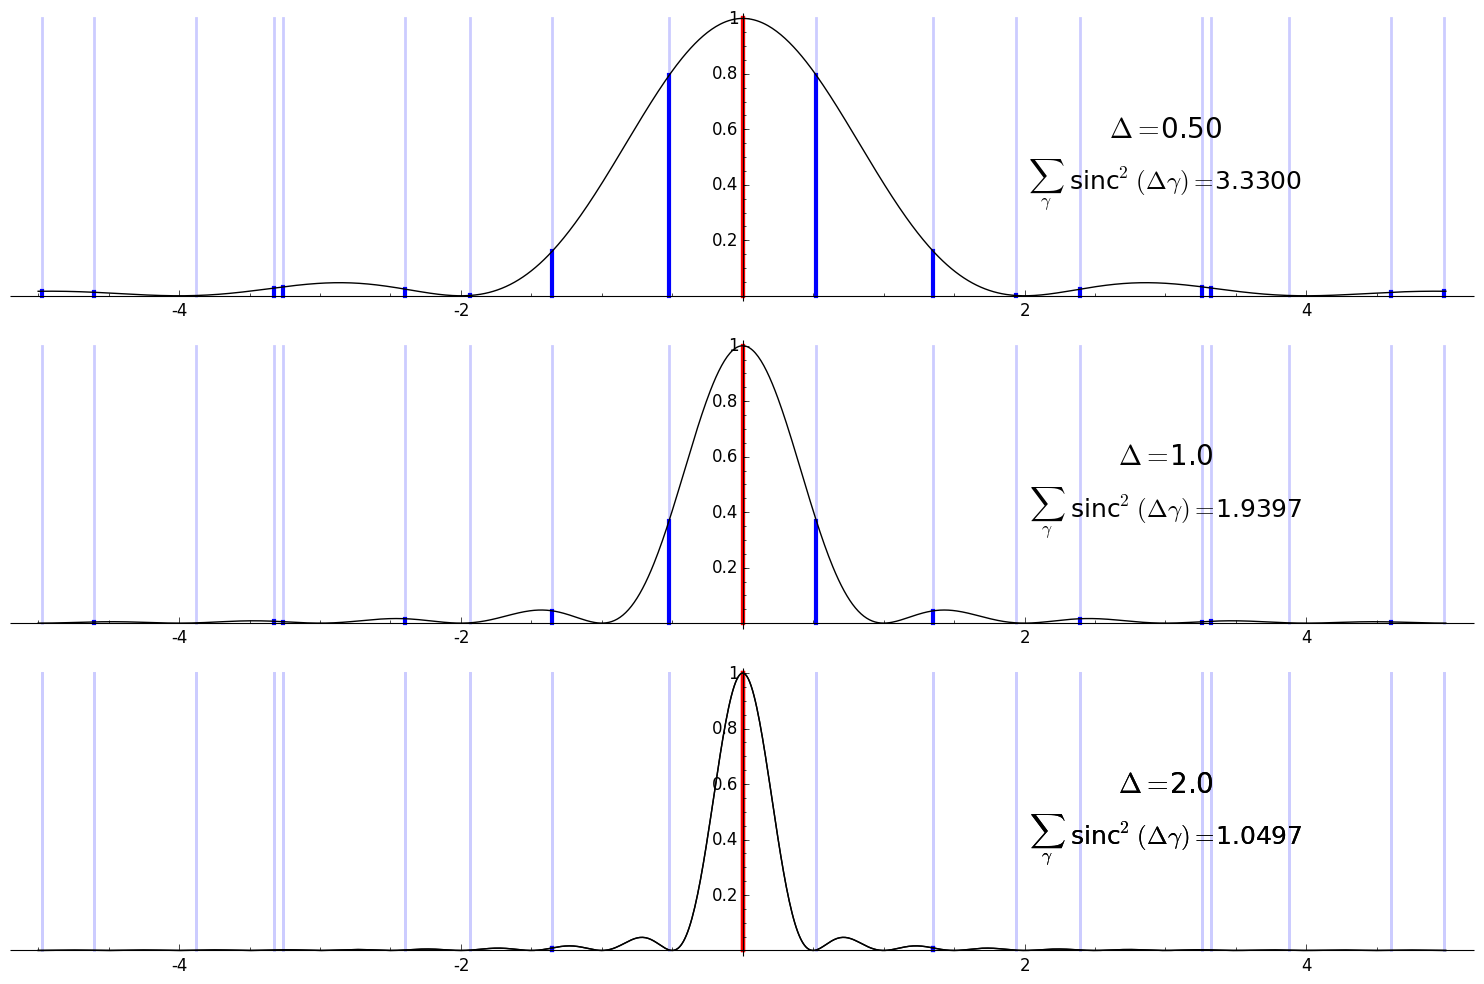
\includegraphics[width=1.0\textwidth]{graphics/zero_sum_visualization.png}
    \caption{A graphic representation of the $\sinc^2$ sum for the elliptic curve $E: y^2=x^3-18x+51$, a rank 1 curve with conductor $N=750384$, for three increasing values of the parameter $\Delta$. Vertical lines have been plotted at $x=\gamma$ whenever $L_E(1+i\gamma)=0$ -- red for the single central zero, and blue for noncentral zeros; the height of the darkened portion of each line is given by the black curve $\sinc^2(\Delta x)$. Summing up the lengths of the dark vertical lines thus gives the value of the $\sinc^2$ sum. We see that as $\Delta$ increases, the contribution from the blue lines -- corresponding to noncentral zeros -- goes to zero, while the contribution from the central zero in red remains at 1. Thus the sum must limit to 1 as $\Delta$ increases.}
    \label{fig:zero_sum_visualization}
\end{figure}

The $\sinc^2$ zero sum rank estimation method has been implemented in Sage (see Appendix A), and used to successfully estimate ranks on a database of 18 million elliptic curves with conductor at most $\sim 10^{11}$. A range of $\Delta$ values was used, from $\Delta=1.0$ (for which average time per curve was $\sim 10^{-5}$ s), to $\Delta=2.0$ (average time per curve $\sim 10^{-1}$ s). See an upcoming paper by Ho, Balakrishnan, Kaplan, Weigandt and S. for details on the computations. \\

A neat conclusion that can immediately be drawn from the finiteness of the $\sinc^2$ explicit formula sum, is that maximum analytic rank grows more slowly than $\log(N)$:

\begin{corollary}\label{cor:rank_slower_than_log_N}
For any $\epsilon >0$ there is a constant $K_{\epsilon}>0$ such that for any $E/\QQ$ with conductor $N$, we have
\begin{equation}
r_{an}(E) < \epsilon \log N + K_{\epsilon}
\end{equation}
\end{corollary}
\begin{proof}
We note that for any given $\Delta>0$, the sum $ \sum_{n<e^{2\pi \Delta}} c_n \cdot \left(1-\frac{\log n}{2\pi \Delta}\right)$ is bounded by a constant that is independent of the choice of elliptic curve, as the $c_n$ values are bounded globally. Thus the right hand side of Equation \ref{eqn:sincsquared_sum} is equal to $\frac{1}{2\pi \Delta}\log N$ plus a number whose supremum magnitude depends only on $\Delta$ and not on $E$. Since the sum bounds analytic rank, taking $\epsilon = \frac{1}{2\pi \Delta}$ and letting $\epsilon \to 0$ proves the statement.
\end{proof}

[Aside: This statement is already known in the literature, so nothing new has been proven here. In fact, it's conjectured that maximum analytic rank grows more like $\sqrt{\log N}$ (existing numerical evidence would seem to support this), but this is still very much an open problem.] \\

The above allows us to provide bounds on analytic rank via point estimates by choosing particular values of $\epsilon$. For example, if we choose $\epsilon = \frac{1}{\log 23} \sim 0.3189\ldots$ and collect and bound all the conductor-independent terms in equation \ref{eqn:sincsquared_sum}, we can improve the result in Corollary \ref{cor:logderiv_rank_bound} to the following:
\begin{corollary}\label{cor:better_an_bound}
Let $E$ have analytic rank $r_E$ and conductor $N_E$. Then
\begin{equation}
r_E < 0.32 \log N_E + 0.5
\end{equation}
\end{corollary}
We leave the details of the proof to the reader as a fun analysis exercise.\\

Finally, it's worth noting is that when $\Delta \le \frac{\log 2}{2\pi}$, the $c_n$ sum in Equation \ref{eqn:sincsquared_sum} is empty. Thus we have the following:
\begin{corollary}
Let $E/\QQ$ have conductor $N$. Let $\eta$ be the Euler-Mascheroni constant $=0.5772\ldots$, and let $\gamma$ range over the nontrivial zeros of $\L_E(s)$. Then
\begin{equation}
\sum_{\gamma} \sinc^2\left(\frac{\log 2}{2\pi} \cdot \gamma \right) = \frac{\log N}{\log 2} + K,
\end{equation}
where $K = \frac{\pi^2}{6(\log 2)^2} - \frac{2\eta}{\log 2} - 2\frac{\log \pi}{\log 2} - 1 = -2.54476987\ldots$ is a global constant that is independent of $E$.
\end{corollary}
\begin{proof}
Evaluate Equation \ref{eqn:sincsquared_sum} at $\Delta = \frac{\log 2}{2\pi}$ and simplify, noting that $\Li_2\left(\frac{1}{2}\right) = \frac{\pi^2}{6} - \frac{(\log 2)^2}{2}$.
\end{proof}

\newpage
%%%%%%%%%%%%%%%%%%%%%%%%%%%%%%%%%%%%%%%%%%%%%%%%%%%%%%%%
\section{Rank Estimation Fidelity and Choosing how to Scale $\Delta$}

Observe that for a fixed choice of $\Delta$, evaluating Equation \ref{eqn:sincsquared_sum} has runtime that is almost independent of the conductor of $E$ (it should scale with some power of $\log N_E$ due to the complexity of basic arithmetic operations). However, as conductor increases the tightness of the provided bound decreases -- we can see this from the first term, which adds a positive bias to the sum proportion to $\log N_E$, which is not seen in the average ranks of curves as conductor increases. \\

\begin{definition}
The {\it fidelity} of a sinc$^2$ sum rank estimation with a given choice of $\Delta$, is the average tightness of the rank bound as a function of conductor of the curve in question. Specifically, we may define
\begin{equation}
\mbox{fid}(\Delta,N) = \mbox{mean}\set{\left(\sum_{\Lambda_E(\gamma)=0}\sinc^2(\gamma \Delta)\right) - r_{an}(E):\;\; N_E = N}
\end{equation}
where $E$ ranges over all rational elliptic curves with conductor $N$. Loosely, we may think of the fidelity of a given choice of $\Delta$ and $N$ to be the expected accuracy of the rank estimate, or the chance that the sum is tight (e.g. within 2 of the true rank, since we are always assuming parity is known) for a curve of conductor $N$. 
\end{definition}

In other words, for fixed curves fidelity increases as $\Delta$ increases, but for fixed $\Delta$ fidelity {\it decreases} as the conductor of the curve in question increases. It follows that $\Delta$ should scale with $N_E$ in order to obtain an estimates of constant fidelity. The natural question to ask then, given the statement of Equation \ref{eqn:sincsquared_sum}, is: how large does $\Delta$ need to be such that $\sum_{\Lambda_E(\gamma)=0}\sinc^2(\gamma \Delta) < r_{an}(E)+2$? \\

Evaluating the sum will be dominated by the final sum over the $c_n$ coefficients, whose runtime in turn is exponential in $\Delta$, so we must be judicious in the choice of $\Delta$. Experimentally, we found that choosing $\Delta(E) = \alpha \cdot \log N_E$ for any constant value of $\alpha$ produces estimates of asymptotically constant fidelity. Such a choice makes the contribution from the first two terms in Equation \ref{eqn:sincsquared_sum} -- $\frac{1}{\Delta \pi}\left(-\eta + \log\left(\frac{\sqrt{N}}{2\pi}\right)\right) + \frac{1}{2\pi^2 \Delta^2}\left(\frac{\pi^2}{6} - \Li_2\left(e^{-2\pi \Delta}\right)\right)$ -- asymptotically constant, so net bias in the sum does not increase as $N_E$ increases. \\

\begin{figure}[!h]
    \centering
    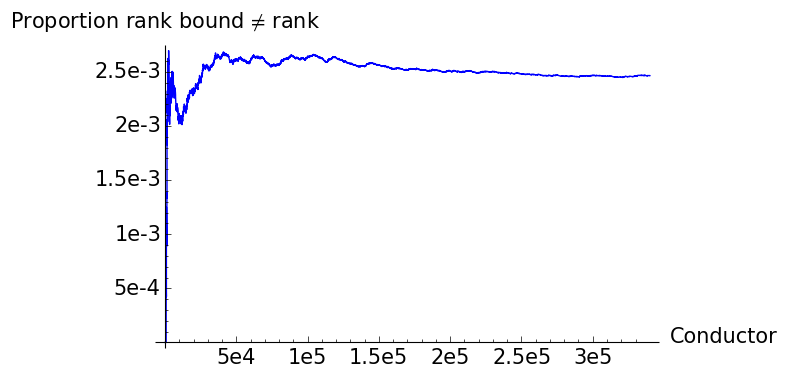
\includegraphics[width=1.0\textwidth]{graphics/rkub_ne_rk.png}
    \caption{The cumulative proportion of curves in the Cremona database for which the sinc$^2$ rank bound was not within 2 of the true rank of the curve, using the scaling $\Delta(E) = \frac{1}{\pi}\left(-\eta + \log\left(\frac{\sqrt{N_E}}{2\pi}\right)\right)$. }
    \label{fig:rkub_ne_rk}
\end{figure}

To generate Figure \ref{fig:rkub_ne_rk}, we used the scaling $\Delta(E) = \frac{1}{\pi}\left(-\eta + \log\left(\frac{\sqrt{N_E}}{2\pi}\right)\right)$, and computed rank bounds on the entire Cremona database of all rational elliptic curves up to conductor 350000; this scaling was chosen so that the bias coming from the first term in the sinc$^2$ sum was always exactly $1$. It was found that the resulting bounds were within 2 of the true rank in 99.75\% of cases. The 4000 or so curves for which the bound exceeded $r_{an}+2$ all possess anomalously low-lying zeros that 'look like central zeros' when small values of $\Delta$ are used. \\

Since the number of terms in the $c_n$ sum in Equation \ref{eqn:sincsquared_sum} is $e^{2\pi\Delta}$, choosing $\Delta(E) = \alpha \cdot \log N_E$ means that the evaluating the sum will have $\softO\left((N_E)^{2\pi \alpha} \right)$ runtime. That is, the scaling choice used to generate Figure \ref{fig:rkub_ne_rk} yielded an $\softO(N_E)$ computation time. In general, runtime can be made to be $\softO\left((N_E)^{\epsilon}\right)$ for any $\epsilon>0$, at the expense of lowering the fidelity of the bound. \\

It is worth noting explicitly that the accuracy of the sinc$^2$ sum rank estimate is sensitive to low-lying zeros. Thus if it known a priori that the $L$-function of a particular curve does not have any low-lying zeros, a smaller value of $\Delta$ can be used. This fact is exploited in \cite{Bob-2011}, where Bober uses the method on curves of very large rank. There is a well-known phenomenon of zero repulsion in $L$-functions -- zeros tend not to fall as close to each other as could be expected if they were distributed purely randomly on the critical line -- and as such curves with large rank tend to have lowest zeros significantly higher up in the upper half plane than would be expected otherwise. \\

This, for example, allowed Bober to use a $\Delta$ value of only $3.2$ to show that a curve with 28 independent points had analytic rank at most 30. The conductor of the curve in question is roughly $3.4\times 10^{141}$, so using the scaling $\Delta(E) = \frac{1}{\pi}\left(-\eta + \log\left(\frac{\sqrt{N_E}}{2\pi}\right)\right)$ would require a $\Delta$ value of about $51.1$.

\newpage
%%%%%%%%%%%%%%%%%%%%%%%%%%%%%%%%%%%%%%%%%%%%%%%%%%%%%%%%
\section{The Distribution of Nontrivial Zeros}

Though not necessary to prove Equation \ref{eqn:sincsquared_sum}, we may also use zero sums to provide estimates on the distribution and expected location of nontrivial zeros of $\Les$ as a function of the curve's conductor. \\

\begin{definition}
For non-negative $t$, let $M_E(t)$ be the modified non-trivial zero counting function for $\Les$, i.e.
\begin{equation}
M_E(t) := \sideset{}{\pr}\sum_{|\gamma| \le t} \frac{1}{2}
\end{equation}
where $\gamma$ runs over the imaginary parts of nontrivial zeros of $L_E(s)$, and the prime indicates that the final $\gamma$ is taken with half weight if $\gamma = t$. The central zero is taken with with multiplicity $r$, where $r$ is the analytic rank of $E$. \\
\end{definition}

Note that $M_E(0) = \frac{r}{2}$, and the function jumps by 1 across the locations of nontrivial zeros, since noncentral zeros come in conjugate pairs and (by GRH) are always simple. \\

\begin{proposition}[S.]
\begin{equation}\label{eqn:M_E(t)}
M_E(t) = \frac{1}{\pi}\left[\left(-\eta+\log\left(\frac{\sqrt{N}}{2\pi}\right)\right) t + \sum_{k=1}^{\infty} \left(\frac{t}{k} - \arctan\left(\frac{t}{k}\right)\right) + \sum_{n=1}^{\infty} \frac{c_n}{\log n}\cdot \sin(t\log n)\right]
\end{equation}
Convergence on the RHS is pointwise with respect to $t$ for both sums; for fixed $t$ convergence for the sums over $k$ and $n$ is absolute and conditional respectively (and {\it extremely} slow for the latter).
\end{proposition}

\begin{proof}
Observe we may write $M_E(t) = \sum_{\gamma}f_t(\gamma)$, where
\begin{equation}
f_t(x) = \begin{cases} \frac{1}{2}, & |x|<t \\ \frac{1}{4}, & |x| = t \\ 0 & |x|> t \end{cases}
\end{equation}
Informally, we obtain the above formula by integrating both sides of Equation \ref{eqn:exp_form_3} against $f = f_t(x)$, noting that $\hat{f}_t(y) = \frac{\sin(ty)}{y}$. The integrals in the sum over $k$ give us no issue and we may swap the order of the integral and summation signs, since convergence there is absolute. However, some care must be taken when it comes to the sum over $n$, since here convergence is only conditional. 

Formally, we must write $M_E(t)$ as a path integral of $\ldLam{1+s}$ on the path
\begin{equation*}
\epsilon-it \mapsto \epsilon+it \mapsto -\epsilon+it \mapsto -\epsilon-it \mapsto \epsilon-it
\end{equation*}
for some $\epsilon>0$, and invoke the Cauchy Residue Theorem. We may then shrink $\epsilon$ to zero (assuming GRH) to obtain that the RHS of \ref{eqn:M_E(t)} converges point wise to $M_E(t)$ as $m$ and $n \to \infty$.
\end{proof}

Equation \ref{eqn:M_E(t)} may be though of having two components. The first two terms comprise a smooth part that gives the ``expected number of zeros'' up to $t$; and the trigonometric sum over $n$ comprises the discretization information that yields the zeros' exact locations. We expect the trigonometric sum to be zero infinitely often, and asymptotically it should be positive as often as it is negative. As such the sum should average out to zero and shouldn't contribute any asymptotic bias to the density of zeros on the critical line. We can therefore talk in a real sense of the expected number of zeros up to $t$, which is given by
\begin{equation}\label{eqn:M_E_smooth_part}
\frac{1}{\pi}\left[\left(-\eta+\log\left(\frac{\sqrt{N}}{2\pi}\right)\right) t + \sum_{k=1}^{\infty} \left(\frac{t}{k} - \arctan\left(\frac{t}{k}\right)\right)\right]
\end{equation}

Moreover, the trigonometric sum should grow very slowly with $t$. Put more formally, we have the following:
\begin{conjecture}\label{conj:trig_sum_size}
\begin{equation}
\sum_{n=1}^{\infty} \frac{c_n}{\log n}\cdot \sin(t\log n) = O(\log t)
\end{equation}
\end{conjecture}
This statement should follow from GRH, and is borne out by numerical evidence:

\begin{figure}[!h]
    \centering
    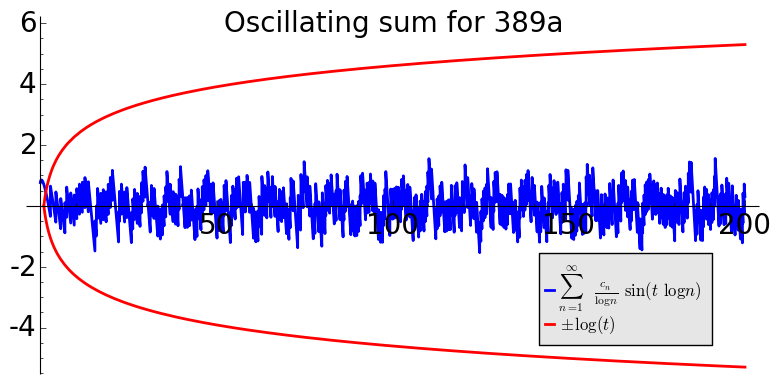
\includegraphics[width=1.0\textwidth]{graphics/M_E_trig_sum_bounds.png}
    \caption{The oscillating sum $\sum_{n=1}^{\infty} \frac{c_n}{\log n}\cdot \sin(t\log n)$ for the curve with Cremona label $389a$ (with equation $y^2 + y = x^3 + x^2 - 2x$) versus $\pm \log(t)$ for $0\le t \le 200$. Numerically we actually see the maximum value of the sum grow slower than $\log(t)$ - possibly $\log(t)^{\alpha}$ for some $0<\alpha<1$, or even $\log\log(t)$.}
    \label{fig:M_E_trig_sum_bounds}
\end{figure}

\begin{lemma}\label{lem:arctan_sum_size}
For $t >> 0$, 
\begin{equation}
\sum_{k=1}^{\infty} \left(\frac{t}{k} - \arctan\left(\frac{t}{k}\right)\right) = t\log t + (\eta-1)t + \frac{\pi}{4} + O\left(\frac{1}{t}\right),
\end{equation}
where $\eta = 0.5772\ldots$ is the Euler-Mascheroni constant.
\end{lemma}
\begin{proof}
We have
\begin{equation*}
\sum_{k=1}^{\infty} \left(\frac{t}{k} - \arctan\left(\frac{t}{k}\right)\right) = \int_{0}^{t} \sum_{k=1}^{\infty} \frac{x^2}{k(k^2+x^2)} \; dx = \int_{0}^{t} \Re\left(\digamma(1+ix) + \eta\right) \; dx,
\end{equation*}
where $\digamma(z)$ is the digamma function on $\CC$. Now along the critical line we have the following asymptotic expansion for the real part of the digamma function:
\begin{equation}
\Re\left(\digamma(1+ix)\right) = \log x + \frac{1}{12} x^{-2} + O(x^{-4})
\end{equation}
Hence $\int_{0}^{t} \Re\left(\digamma(1+ix)\right) \; dx = t(\log t - 1)  + O(1)$. The constant term of $\frac{\pi}{4}$ comes from integrating the difference between $\Re\left(\digamma(1+ix)\right)$ and $\log x$ between $0$ and $\infty$:
\begin{equation*}
\int_{0}^{\infty} \left[\Re\left(\digamma(1+ix)\right) - \log x\right] \; dx = \frac{\pi}{4}.
\end{equation*}
The result follows.
\end{proof}

Conjecture \ref{conj:trig_sum_size} and lemma \ref{lem:arctan_sum_size} combine to give us a precise asymptotic statement on the distribution of zeros up to $t$, in the same vein as von Mangoldt's asymptotic formula for the number of zeros up to $t$ for $\zeta$:

\begin{theorem}[S.]\label{thm:zero_density}
Let $E$ have conductor $N$. Then for $t>>0$ we have
\begin{equation}\label{eqn:zero_density}
M_E(t) = \frac{t}{\pi} \, \log\left(\frac{t\sqrt{N}}{2\pi e}\right) + \frac{1}{4} + O(\log t),
\end{equation}
where the error term is positive as often as it negative and contributes no net bias.
\end{theorem}

\begin{figure}[!h]
    \centering
    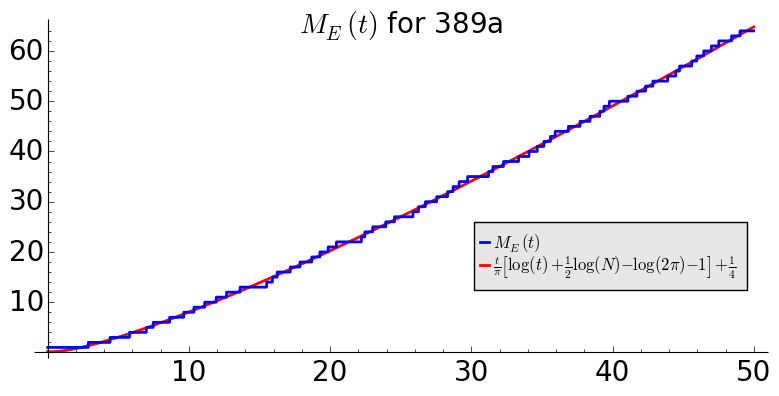
\includegraphics[width=1.0\textwidth]{graphics/M_E_389.png}
    \caption{The number of zeros up to $t$ versus $\frac{t}{\pi}\left[\log\left(\frac{t\sqrt{N}}{2\pi}\right) -1 \right] + \frac{1}{4}$ for the Cremona curve $389a$. The match up is extremely good.}
    \label{fig:M_E_389}
\end{figure}

\begin{corollary}
For $t>>0$, the number of zeros on the critical line in a unit interval
\begin{equation}
M_E(t)-M_E(t-1) = \frac{1}{\pi}\log\left(\frac{t\sqrt{N}}{2\pi}\right) + O(\log t),
\end{equation}
where again the error term contributes no net bias.
\end{corollary}

That is, zero density on the critical line grows like $\frac{1}{2}\log N + \log t$, where $N$ is the conductor of $E$ and $t$ the distance from the real axis. \\

Neglecting the oscilating error term in Equation \ref{eqn:zero_density}, we may solve for $t$ in terms of the Lambert $W$-function to obtain an explicit formula for the expected value of the imaginary part of the $n$th zero on the critical line. Recall the definition of the Lambert $W$-function: if $y = x e^x$, then $x = W(y)$. $W$ is a multiple-valued function; we make use of the principle branch $W_0$ below:
\begin{corollary}
Let $\gamma_n := \gamma_n(E)$ be the imaginary value of the $n$th nontrivial (and noncentral) zero in the upper half plane of $\Les$ with analytic rank $r$. Then
\begin{equation}\label{approx:gamma_n}
\gamma_n \sim \frac{2\pi e}{\sqrt{N}} \cdot \exp \left(W_0\left[\left(\frac{r}{2} +n - \frac{3}{4}\right)\cdot \frac{\sqrt{N}}{2 e}\right]\right)
\end{equation}
in the sense that for a given curve, the difference between the above value and the true value of $\gamma_n$ will on average be zero as $n \to \infty$.
\end{corollary}
\begin{proof}
Observe that the $n$th nontrivial noncentral zero has imaginary part $t$ when $M_E(t) = \frac{r}{2} + n - \frac{1}{2}$ (since the final zero is counted with half weight). Hence using Equation \ref{eqn:zero_density} sans the oscillating error term, we solve for $t$ in
\begin{equation*}
\frac{t}{\pi} \, \log\left(\frac{t\sqrt{N}}{2\pi e}\right) + \frac{1}{4} = \frac{r}{2} + n - \frac{1}{2}
\end{equation*}
\end{proof}

[Aside: The principle branch of the Lambert $W$-function has the asymptotic expansion $W_0(x) = \log x - \log \log x + o\left(1\right)$, for $n >> 0$ we recover the known asymptotic for the location of the $n$th nontrivial zero: $\gamma_n = O\left(\frac{n}{\log n} \right)$. Better yet, after some manipulation the asymptotic expansion gives us the proportionality constant explicitly:
\begin{equation}
\lim_{n \to \infty} \frac{\gamma_n}{\frac{n}{\log n}} = \pi
\end{equation}
Note, however, that the convergence rate is slow: $O(\frac{1}{\log n})$, and the constant in front scales with the log of the conductor of $E$.] \\

A natural question to ask, given that we now have an expected value for $\gamma_n$, is: how much does the imaginary part of the $n$th zero deviate from its expected location? To this end we define the {\it dispersion} of the $n$th zero:
\begin{definition}
The dispersion $\delta_n(E) := \delta_n$ of the imaginary part of the $n$th nontrivial zero in the upper half plane is the difference between the true and predicted values of $\gamma_n$, i.e.
\begin{equation}
\delta_n = \gamma_n - \frac{2\pi e}{\sqrt{N}} \cdot \exp \left(W_0\left[\left(\frac{r}{2} +n - \frac{3}{4}\right)\cdot \frac{\sqrt{N}}{2 e}\right]\right)
\end{equation}
\end{definition}

\begin{figure}[!h]
    \centering
    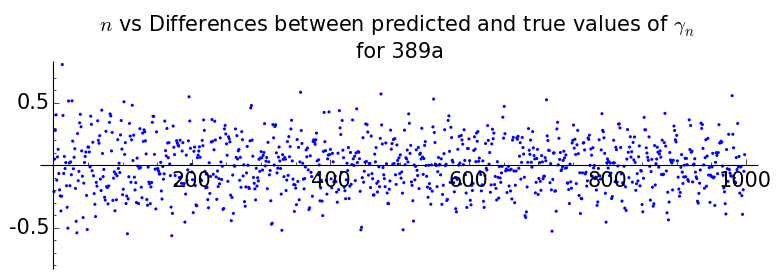
\includegraphics[width=1.0\textwidth]{graphics/389a_zero_dispersions_scatterplot.png}
    \caption{A scatter plot of zero dispersions for the first 1000 nontrivial zeros of the Cremona curve 389a, the rank 3 curve with smallest conductor. The values are seldom more than $\frac{1}{2}$.}
    \label{fig:389a_zero_dispersions_scatterplot}
\end{figure}

\begin{figure}[!h]
    \centering
    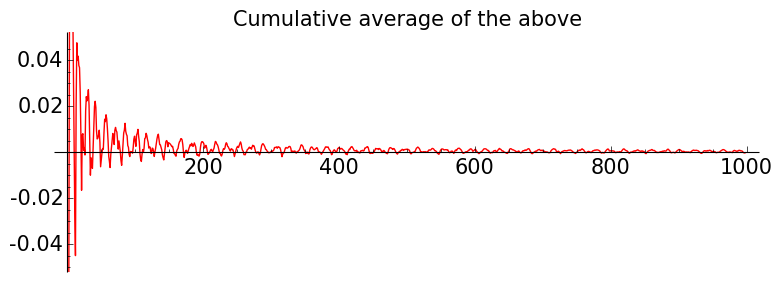
\includegraphics[width=1.0\textwidth]{graphics/389a_zero_dispersions_cumulative_average.png}
    \caption{A cumulative average plot of the above, showing clearly that asymptotically, the average difference between the predicted and true values of $\gamma_n$ is zero. The positive bias at the beginning comes from the $O(1/t)$ term in Lemma \ref{lem:arctan_sum_size}. Interestingly, although the deviations might a priori appear completely random, there is a clear oscillating structure in the average, and the line about which the oscillation occurs appears to decrease to zero from above.}
    \label{fig:zero_dispersions_cumulative_average}
\end{figure}

Even though the above graph demonstrates that the zero dispersions are clearly not random, when viewed as a i.i.d. time series, the dispersions appear be normally distributed. \\

\begin{figure}[!h]
    \centering
    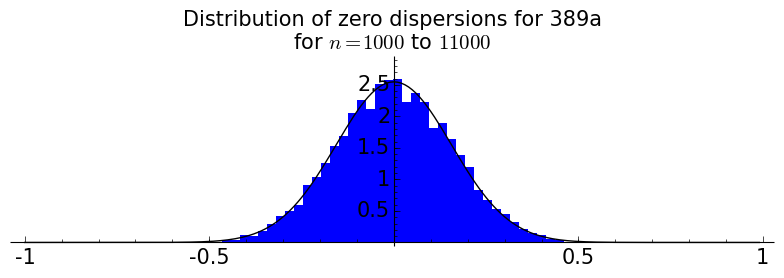
\includegraphics[width=1.0\textwidth]{graphics/389a_zero_dispersions_histagram.png}
    \caption{A histogram of zero dispersions for the curve 389 for the 1000th through 11000th zeros (we discard the first 1000 zeros to avoid the small-height bias observable in the the cumulative average plot above). }
    \label{fig:389a_zero_dispersions_histagram}
\end{figure}

For the data set used the graph above, the mean was $3.16\times10^{-5}$ (a good indicator that the expected value formula contains no systematic bias), standard deviation $0.1566$. The standard deviation appears to decrease with increasing $n$: we applied the Shapiro-Wilk normality test on batches of 1000 consecutive zero dispersions, and got $p$-values in excess of $0.2$ (and most of the time in excess of 0.5) in all cases. Moreover, the computed standard deviations decreased uniformly from $0.1745$ for the $n=1000$ to $2000$ dispersion set, to $0.1464$ in the $n=10000$ to $11000$ set. We hope to pursue this investigation in future work. \\

Finally, we may also go in the other direction and use Equation \ref{eqn:M_E(t)} to make a guess as to the expected imaginary part of the {\it lowest} noncentral nontrivial zero of $\Les$ as a function of increasing conductor $N$:
\begin{proposition}
For a curve $E$ with large conductor $N$, the best guess for the imaginary part of the first nontrivial noncentral zero $\gamma_1$ of $\Les$ in the upper half plane is
\begin{equation}
\gamma_1 = \frac{(r+1)\pi}{\log(N) -2\log(2\pi) -2\eta}
\end{equation}
where $r$ is the analytic rank of $E$
\end{proposition}
The derivation is similar to before. The location of the first nontrivial noncentral zero is given by the value of $t$ for which $M_E(t)$ jumps from $r/2$ to $r/2+1$; at that point $M_E(t) = r/2 + 1/2 = \frac{r+1}{2}$, so the expected value of $\gamma_1$ is given by setting equation \ref{eqn:M_E(t)} equal to $\frac{r+1}{2}$ and solving for $t$. \\

Now, however, $\frac{1}{\pi}\sum_{k=1}^{\infty} \left[\frac{t}{k} - \arctan\left(\frac{t}{k}\right)\right]$ is $O(t^3)$ for small t, so the quantity expressed in equation \ref{eqn:M_E_smooth_part} is dominated by the $\frac{1}{\pi}\left(-\eta+\log\left(\frac{\sqrt{N}}{2\pi}\right)\right) t$ term when $N$ is large. Solving for $t$ yields the desired value.

\newpage
%%%%%%%%%%%%%%%%%%%%%%%%%%%%%%%%%%%%%%%%%%%%%%%%%%%%%%%%
\section{The Bite}

Recall by Definition \ref{defn:bite}, the {\it bite} $\beta_E$ of an elliptic curve is given by
\begin{equation}
\beta_E = \sum_{\gamma \ne 0} \frac{1}{\gamma^2}
\end{equation}
where $\gamma$ ranges over the imaginary parts of the {\it non-central} nontrivial zeros of $\Les$. In this sections we establish some bounds on the bite, show how one can compute it efficiently without having to compute the locations of the zeros of $\Les$ explicitly, and finish off with a result showing that the lowest noncentral zero is bounded away from the central point in terms of a negative power of the conductor. \\

%It is a relatively straightforward affair to obtain unconditional upper bounds on the magnitude of $C_E$, the central leading coefficient of $\Les$, as a function of the curve's conductor; this can be achieved by doing some analysis on $\ldLam{1+s}$ and the bite $\beta_E$. Lower bounds are more difficult, however. It is only by assuming full BSD that we have any way of obtain $C_E$ from below. \\

As zero density on the critical line grows proportional to $\frac{1}{2}\log N_E$ (see Theorem \ref{thm:zero_density}), we expect the bite to grow like $\frac{1}{2}\log N_E$ too. This is indeed the case, at least in terms of concrete lower bounds on $\beta_E$:
\begin{lemma}[S.]
For all $\epsilon>0$ there is a constant $K(\epsilon)>0$ such that for all elliptic curves $E$, the bite of $E$ obeys
\begin{equation}
\beta_E = \sum_{\gamma\ne 0} \frac{1}{\gamma^2} > \frac{1}{2+\epsilon} \log N_E - K(\epsilon).
\end{equation}
where $N_E$ is the conductor of $E$.
\end{lemma}
\begin{proof}

\end{proof}

\begin{proposition}\label{prop:bite_times_leading_coeff}
Let $E$ have completed $L$-function $\Lams$ and analytic rank $r$. Then
\begin{equation}
\beta_E\cdot C_E = \frac{\Lambda_E^{(r+2)}(1)}{(r+2)!},.
\end{equation}
where $\beta_E$ is the bite of $E$, and $C_E$ is the leading coefficient of $\Lams$ at the central point.
\end{proposition}
\begin{proof}
From equation \ref{eqn:Lams_prod} we have that 
\begin{equation}
\Lambda_E(1+s) = C_E\left(s^r + \beta_E s^{r+2} + O(s^{r+4})\right)
\end{equation}
Differentiating $r+2$ times and evaluating at $s=0$ achieves the desired result.
\end{proof}

From this we derive a straightforward way to compute the bite of $E$ from the $r$th and $(r+2)$th Taylor coefficients of the $L$-series attached to $E$ (this of course relies on knowing the analytic rank of $E$):
\begin{corollary}
\begin{align}
\beta_E \quad &= \frac{1}{(r+1)(r+2)} \cdot \frac{\Lambda_E^{(r+2)}(1)}{\Lambda_E^{(r)}(1)} \\
&= \frac{2}{(r+1)(r+2)} \cdot \frac{L_E^{(r+2)}(1)}{L_E^{(r)}(1)} - \left(-\eta+\log\left(\frac{\sqrt{N}}{2\pi}\right)\right)^2 + \frac{\pi^2}{6}
\end{align}
\end{corollary}
\begin{proof}
The first line follows immediately from Proposition \ref{prop:bite_times_leading_coeff} and the fact that $C_E = \frac{\Lambda^{(r)}(1)}{r!}$. The second line comes from the formula for the $(r+2)$th Taylor coefficient of $L_E$ at the central point derived in Corollary \ref{cor:ldLe_expansion}.
\end{proof}
This allows us to compute the bite of a curve {\it without} having to compute the locations of the zeros themselves. Moreover, the bite can be computed to arbitrary precision in polynomial time (in the conductor and the number of bits of precision) using, for example, Tim Dokchitser's {\tt computel} PARI code, which can compute the Taylor series expansion of a motivic $L$-function at a given point. [Important side-note: the aforementioned package uses approximations that have not (yet) been shown to be provably correct; however, one one could certainly write code to compute in polynomial time the central Taylor expansion of $\Les$ via the work of Bradshaw in \cite{Bra-2010}, which {\it does} produce provably correct $L$-function values.] \\

\begin{figure}[!h]
    \centering
    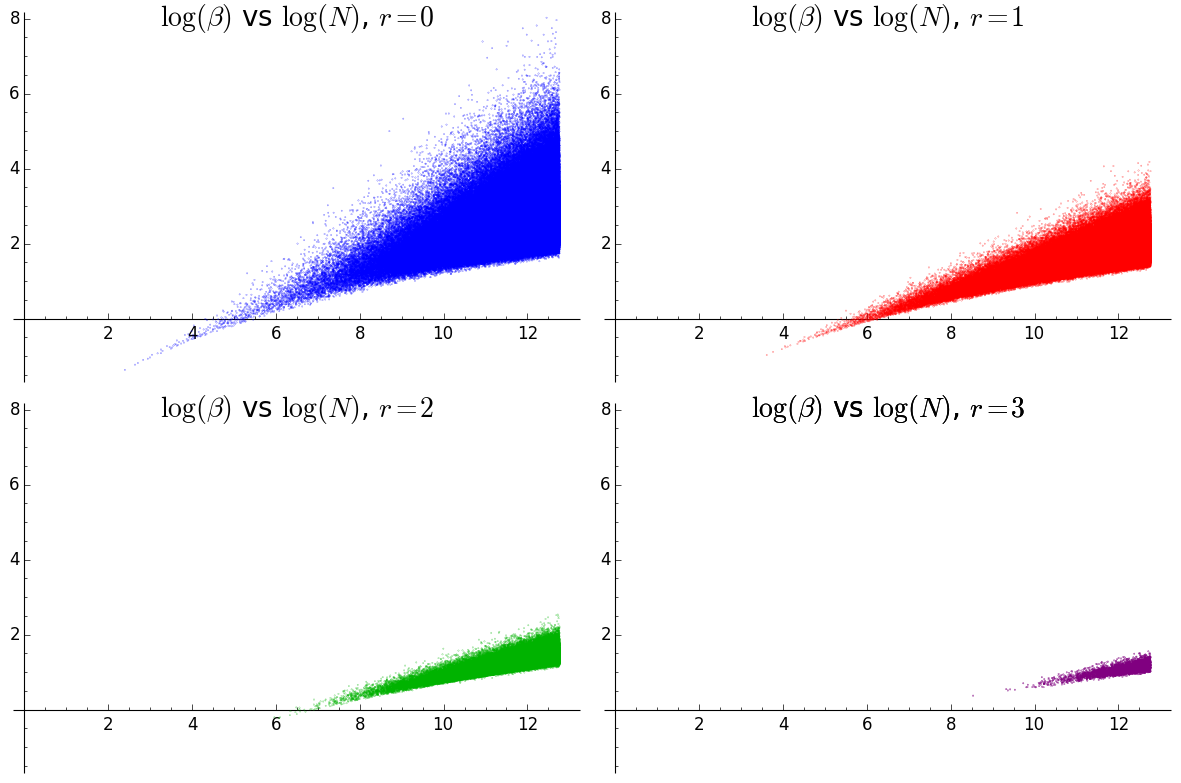
\includegraphics[width=1.0\textwidth]{graphics/bites_vs_conductors_array.png}
    \caption{The bites of all curves in the Cremona tables were computed using the above method. Above is a plot of $\log(\beta)$ vs. $\log(N)$ for curves of rank 0, 1, 2 and 3 respectively. }
    \label{fig:bites_vs_conductors_array}
\end{figure}

One can see from he above plot that the bite obeys a sharp lower bound with respect to the conductor, but the upper bound is somewhat less tight. More interesting is the fact that the lower bound appears the same regardless of rank, while curves with anomalously large bits are predominantly rank $0$. This makes sense: large bites correspond to very low-lying zeros, and because of the well-documented zero repulsion effect, this can only really happen when there are no zeros at the central point. \\

%%%%% INCLUDE PICTURES OF BITE VS. CONDUCTOR AND LEADING COEFF HERE %%%%%

To establish bounds on the coefficients of the Taylor expansion of $\Lams$ about the central point, we will need the following technical lemma:
\begin{lemma}\label{lem:central_deriv_int_bounds}
Let $N,n \in \ZZ_{>0}$, and suppose $k$ is a positive integer such that $k < \frac{1}{2}\log N$. Then
\begin{equation}
\left| \int_{\frac{1}{\sqrt{N}}}^{\infty} (\log t)^{k} e^{-2\pi n t} \; dt \right| < \frac{\left(\frac{1}{2} \log N\right)^{k}}{2\pi n}\left[ e^{-\frac{2\pi n}{\sqrt{N}}} + \frac{e^{-2\pi n\sqrt{N}}}{2\pi n \sqrt N} \right].
\end{equation}
\end{lemma}
\begin{proof}
We split the integral in two, dealing with the intervals $\frac{1}{\sqrt{N}}$ to $\sqrt{N}$ and $\sqrt{N}$ to $\infty$ separately. Now $(\log t)^{k}$ is at most $(\frac{1}{2}\log N)^k$ in magnitude on $[\frac{1}{\sqrt{N}},\sqrt{N}]$, so
\begin{equation*}
\left| \int_{\frac{1}{\sqrt{N}}}^{\sqrt{N}} (\log t)^{k} e^{-2\pi n t} \; dt \right| < \left(\frac{1}{2} \log N\right)^k \int_{\frac{1}{\sqrt{N}}}^{\sqrt{N}} e^{-2\pi n t} \; dt < \frac{\left(\frac{1}{2} \log N\right)^{k}}{2\pi n}\left(e^{-\frac{2\pi n}{\sqrt{N}}} - e^{-2\pi n\sqrt{N}}\right)
\end{equation*}
For the integral on $[\sqrt{N},\infty)$, we use integration by parts to get
\begin{equation*}
\int_{\sqrt{N}}^{\infty} \left(\log t \right)^{k} e^{-2\pi n t} \; dt = \frac{\left(\frac{1}{2} \log N\right)^{k}}{2\pi n}\cdot e^{-2\pi n\sqrt{N}} + \frac{k}{2\pi n} \int_{\sqrt{N}}^{\infty} \frac{\left(\log t \right)^{k-1}}{t} e^{-2\pi n t} \; dt 
\end{equation*}
If $k < \frac{1}{2}\log N$, then $\frac{\left(\log t \right)^{k-1}}{t}$ is decreasing for $t > \sqrt{N}$, so we have
\begin{equation*}
\frac{k}{2\pi n} \int_{\sqrt{N}}^{\infty} \frac{\left(\log t \right)^{k-1}}{t} e^{-2\pi n t} \; dt < \frac{k\left(\frac{1}{2} \log N\right)^{k-1}}{2\pi n\sqrt{N}} \int_{\sqrt{N}}^{\infty} e^{-2\pi n t} \; dt < \frac{\left(\frac{1}{2} \log N\right)^{k}}{(2\pi n)^2 \sqrt{N}} \cdot e^{-2\pi n \sqrt{N}}.
\end{equation*}
Add up all the values and you get the established result.
\end{proof}

With the above lemma in hand, we establish an upper bound on the magnitude of the $k$th Taylor coefficient of $\Lams$ at the central point.
\begin{proposition}\label{prop:central_deriv_bounds}
Let $E$ have conductor $N$ and completed $L$-function $\Lams$. Then so long as $k<\frac{1}{2}\log N$, the $k$th derivative of $\Lams$ at the central point is bounded explicitly in terms of $N$ and $k$ by
\begin{equation}
\left| \Lambda_E^{(k)}(1)\right| < \frac{(\frac{1}{2}\log N)^k}{2\pi^2}\left(N + \frac{1}{e^{2\pi\sqrt{N}}-1} \right).
\end{equation}
That is, for fixed $k$ the $k$th Taylor coefficient of $\Lams$ is $O\left( N(\frac{1}{2}\log N)^k\right)$; the second term inside the final parentheses is negligible for $N>>1$.
\end{proposition}

\begin{proof}
From Lemma \ref{lem:central_deriv_int_bounds} and Equation \ref{eqn:lambda_derivs} we have that
\begin{equation*}
\left| \Lambda_E^{(k)}(1)\right| < 2 \sqrt{N} \sum_{n=1}^{\infty} |a_n| \cdot \left[\frac{\left(\frac{1}{2} \log N\right)^{k}}{2\pi n}\left( e^{-\frac{2\pi n}{\sqrt{N}}} + \frac{e^{-2\pi n\sqrt{N}}}{2\pi n \sqrt N} \right)\right]
\end{equation*}
Using the bound $|a_n(E)| \le n$ for any $E$, we get
\begin{equation*}
\left| \Lambda_E^{(k)}(1)\right| < \frac{ \sqrt{N}\left(\frac{1}{2} \log N\right)^{k}}{\pi} \sum_{n=1}^{\infty} e^{-\frac{2\pi n}{\sqrt{N}}} + \frac{\left(\frac{1}{2} \log N\right)^{k}}{2\pi^2} \sum_{n=1}^{\infty} \frac{e^{-2\pi n\sqrt{N}}}{n}
\end{equation*}
Now
\begin{equation*}
\sum_{n=1}^{\infty} e^{-\frac{2\pi n}{\sqrt{N}}} = \frac{1}{e^{\frac{2\pi n}{\sqrt{N}}}-1}< \frac{\sqrt{N}}{2\pi},
\end{equation*}
while $\sum_{n=1}^{\infty} \frac{e^{-2\pi n\sqrt{N}}}{n} \le \sum_{n=1}^{\infty} e^{-2\pi n\sqrt{N}} = \frac{1}{e^{2\pi\sqrt{N}}-1}$.
\end{proof}

Note that for fixed $N$, if we allow $k \to \infty$, we actually have that the $k$th derivative can grow like $O\left(\frac{k!!}{(2\pi e)^{k/2}}\right)$, where $k!! = k(k-2)\cdots$ is the double factorial on $k$ - i.e., faster than exponentially in $k$. However, this behavior only starts to show when $k>>\log N$ - hence our restriction on the magnitude of $k$. This will in practice never be an issue: we are primarily interested in the central derivatives in order to establish results about the analytic rank of $E$. Since maximum analytic rank grows more slowly than $\log N$ (c.f. Corollary \ref{cor:logderiv_rank_bound}), we will never need to consider $\Lambda_E^{(k)}(1)$ for $k> \frac{1}{2}\log N$.

% ========== Chapter 6
\chapter{Remarks and Future Work}
% ----- CHAPTER 6: REMARKS AND FUTURE WORK ----- %

This dissertation pulls in results from a number of disparate topics related to elliptic curves, with the general approach being ``do enough to establish results that are sufficient to support the main theorems, then move on". As such, many of the bounds and statements obtained of the course of this work are very far from optimal, and the ultimate running time of, say, Algorithm \ref{algo:compute_rank} could be considerably improved if these bounds were tightened. Beyond this there are natural generalizations to the results in this work that should be considered, We list below the areas where results could be improved upon or generalized, and in so doing detail directions for possible future work.

%%%%%%%%%%%%%%%%%%%%%%%%%%%%%%%%%%%%%%%%%%%%%%%%%%%%%%%
\subsection{Implementing and optimizing the rank algorithm}

I coded up a na\"{i}ve implementation of Algorithm \ref{algo:compute_rank} in Sage to collect supporting data for inclusion in this dissertation, but the algorithm is calling out for a dedicated optimized implementation for general use. Much of the hard work has already been done -- for example, Bradshaw provided a Sage implementation of provable motivic $L$-function evaluation in \cite{Bra-2010}, and Sage already includes functionality to compute the real period of an elliptic curve. \\

There are several optimizations that should be included in any implementation. Three which immediately spring to mind are as follows:
\begin{itemize}
\item One should check for torsion on $E$, which is quick to do. Doing so results in up to 16 less bits of precision needed when evaluating $L_E(s)$.
\item It might be advantageous to compute the Tamagawa product $\prod_p c_p$ if it can be quickly done. Again, this results in a larger lower bound on the leading Taylor coefficient of $C_E$, and thus less precision needed when evaluating $L_E(s)$.
\item The $r_{an}(E) < a\log N_E + b$ bounds used for analytic rank are in practice far too crude; in reality the vast majority of curves (if you believe the folklore conjecture, asymptotically 100\%) have rank 0 or 1, and maximum observed rank goes more like $\sqrt{\log N_E}$. It therefore makes sense to obtain a better upper bound on the rank of a given curve up front; this then gives a better lower bound on the regulator and thus further reduces the required precision when provably evaluating $L_E(s)$. One could, for example, run the $\sinc^2$ sum algorithm exhibited in Section \ref{sec:sinc_squared_sum} with some small choice of $\Delta$, which doesn't require direct evaluation of $L_E(s)$.
\end{itemize}

%%%%%%%%%%%%%%%%%%%%%%%%%%%%%%%%%%%%%%%%%%%%%%%%%%%%%%%
\subsection{Generalizing results to modular $L$-functions of arbitrary weight and level}

The results in this thesis revolve around working with the $L$-function attached to a given elliptic curve. By the modularity theorem \cite{BCDT-2011}, each of these is actually the $L$-function attached to a certain weight 2 integral cuspidal eigenform of level $N_E$, where $N_E$ is the conductor of the curve in question. \\

In general we can attach an $L$-function to a cuspidal eigenform of arbitrary weight and level. Many of the results in this dissertation should carry over naturally, allowing us address the issue of computing the analytic rank of higher-weight modular $L$-functions. Specifically, given an analogue of BSD we should be able to show that an algorithm exists to compute the analytic rank of a modular $L$-function that is polynomial-time in the level of that form. An immediate question would then be: how does such a method scale with the {\it weight} of the form? \\

Moreover, the $\sinc^2$ zero sum method to bound analytic rank from above should transfer directly to higher weight forms. We hope in future to extend the functionality of the Sage code to accommodate for this -- in fact, the code layout was designed with this extensibility explicitly in mind.

%%%%%%%%%%%%%%%%%%%%%%%%%%%%%%%%%%%%%%%%%%%%%%%%%%%%%%%
\subsection{CM curves and families of quadratic twists}

Two related questions that we can ask are:
\begin{itemize}
\item Can we get better bounds and results if we restrict ourselves to considering CM curves?
\item Do there exist optimizations for Algorithm \ref{algo:compute_rank} and other results if we consider the family of quadratic twists of a given elliptic curve? How does complexity scale with the twisting parameter $d$?
\end{itemize}

In both cases, we should ask the question: how do the BSD invariants (especially the regulator and real period) vary within a given family? At the very least the real periods within a family of twists is very rigidly controlled, so we should for be able to write down the required precision in Algorithm \ref{algo:compute_rank} as a function of conductor without needing to compute the real period for each curve. \\

Some work has already gone into considering the case of quadratic twists of a given curve -- see \cite{DeRo-2007}. It would be interesting to see if these ideas could be incorporated to improve the results in this thesis.

%%%%%%%%%%%%%%%%%%%%%%%%%%%%%%%%%%%%%%%%%%%%%%%%%%%%%%%
\subsection{Bounding analytic rank from above in terms of conductor}

To establish a lower bound on the regulator of an elliptic curve in terms of its conductor we require an upper bound on the analytic rank. To this end we invoke Corollaries \ref{cor:logderiv_rank_bound} and \ref{cor:better_an_bound}, stating that maximum analytic rank is bounded by a constant times $\log N_E$ plus another explicit constant. \\

However, Corollary \ref{cor:rank_slower_than_log_N} asserts that, contingent on GRH, maximum analytic rank of in fact grows slower than any multiple of $\log N_E$. We would like to use this result more effectively, but the issue lies in making the constant $K_\epsilon$ explicit in terms of the $\epsilon$ chosen. This translates to bounding the $c_n$ sum
\begin{equation}
\sum_{n < e^{2\pi \Delta}} c_n \cdot \left(1-\frac{\log n}{2\pi \Delta}\right)
\end{equation}
in terms of the parameter $\Delta$. \\

A natural question we can ask, and hopefully answer, is ``can this be done effectively"? Empirically, the $c_n$ sum is seldom more than a handful of units in magnitude; however, the fact that the sum is carried out over prime powers and large amounts of cancellation due to the changing signs of the $c_n$ coefficients means that this term is tricky to control [note that one can readily obtain a naive explicit bound that is exponential in $\log \Delta$, but this is of limited practical use]. \\

Nevertheless, if one could show that the sum grows at most polynomial in $\log \Delta$ (regardless of $E$) and obtain explicit constants, then we should be able to show that the lower bound on the regulator of $E$ would go to zero more slowly than any negative power of $N$, as appears to be the case in practice. \\

%%%%%%%%%%%%%%%%%%%%%%%%%%%%%%%%%%%%%%%%%%%%%%%%%%%%%%%
\subsection{The regulator}

The lower bound on $\Reg_E$ could potentially be improved in multiple ways. Firstly, the result relies on the Hindry-Silverman/Elkies' result \cite{Elk-2006} that, contingent on ABC, for any rational point $P$ on curve $E$ with discriminant $D_E$ obeys
\begin{equation}
\hat{h}(P) > M_0 \log(D_E),
\end{equation}
where $M_E \ge 3.94\times 10^{-5}$. This result is in all probability not optimal. An improvement in the lower bound on point height would result in a direct improvement on the constants involved in the lower bound on the regulator, and thus the precision required in the evaluation of $L_E(s)$ in Algorithm \ref{algo:compute_rank}. Again, this is a deep topic, so new insight here won't come easily. \\

What is perhaps a bit more tractable is to continue in the same vein as in the beginning of the proof of Theorem \ref{thm:regulator_lower_bound}: artificially increase the size of the constant, and check computationally that it holds for all curves up to a given conductor bound. We chose a bound of $N=350000$ simply because that is where Cremona's tables currently go to, but there is no theoretical reason one has to stop there. This option of course pays the price of being computationally much more tedious. \\

Finally, the lower bound on $\Reg_E$ contains a reciprocal Gamma factor, which means that the lower bound decays faster than any power of $\log N_E$. This factor arises from the lower bound on the minimum covolume of a lattice in $\RR^r$ with a fixed minimum vector length (Lemma \ref{lem:covolume_lower_bound}), which is most likely not optimal. If a better lower bound could be exhibited on Lattice covolume as a function of dimension, it is conceivable that we could eliminate the Gamma factor entirely. This is desirable, as we would then have that $\Reg_E$ is bounded below by a negative power of the conductor.

%%%%%%%%%%%%%%%%%%%%%%%%%%%%%%%%%%%%%%%%%%%%%%%%%%%%%%%
\subsubsection{The real period}

The lower bound on the real period of an elliptic curve could potentially be improved further. Specifically, in  we would like to make the constant in Theorem \ref{thm:real_period_lower_bound} completely explicit as a function of $\epsilon$, which would remove the need to compute $\Omega_E$ in order to determine the precision. \\

Secondly, the bound of $\Reg_E > K_{\epsilon}\cdot (N_E)^{-1.5-\epsilon}$ does not seem to be very tight; empirically it would appear that minimum real period goes more like $(N_E)^{-1}$. It would be useful to see if the proofs in Section \ref{sec:real_period} could be reworked to make the results conform more closely with the observed data.


%We invoke ABC and Szpiro's Conjecture when proving lower bounds on the real period in terms of the conductor; however, this isn't strictly necessary. Since the minimal discriminant of a rational elliptic curve is $12$th-power free (outside of $2$ and $3$), there is a natural power bound of the minimal discriminant in terms of the conductor:
%\begin{equation}
%|D_E| \le K\cdot \left(N_E\right)^{12},
%\end{equation}
%where $K$ is an explicit constant that accounts for the potentially higher powers of $2$ and $3$ (which can and should be easily made explicit). As such, we should be able to completely remove the dependence on Szpiro in Theorem \ref{thm:real_period_lower_bound}, at the expense of having less optimal constants. \\
%
%Note that this line was deliberately not pursued in this dissertation, as the assumption of ABC is required for bounds on the regulator in any case. However, ultimately we would like to remove reliance on ABC (if possible) entirely; bounds on the real period are not the obstruction when it comes to this.

%%%%%%%%%%%%%%%%%%%%%%%%%%%%%%%%%%%%%%%%%%%%%%%%%%%%%%%
\subsection{Convergence rate and and convexity statements on the sinc$^2$ rank bounding sum}

Equation \ref{eqn:sincsquared_sum} gives the analytic rank of $E$ as a limit:
\begin{align}
r_E = \quad & \lim_{\Delta \to \infty} \;\; \frac{1}{\Delta \pi}\left[\left(-\eta + \log\left(\frac{\sqrt{N}}{2\pi}\right)\right)+ \frac{1}{2\pi \Delta}\left(\frac{\pi^2}{6} - \Li_2\left(e^{-2\pi \Delta}\right)\right)  \right. \nonumber \\
&+ \left.\sum_{n<e^{2\pi \Delta}} c_n \cdot \left(1-\frac{\log n}{2\pi \Delta}\right)\right].
\end{align}

\begin{figure}[!h]
    \centering
    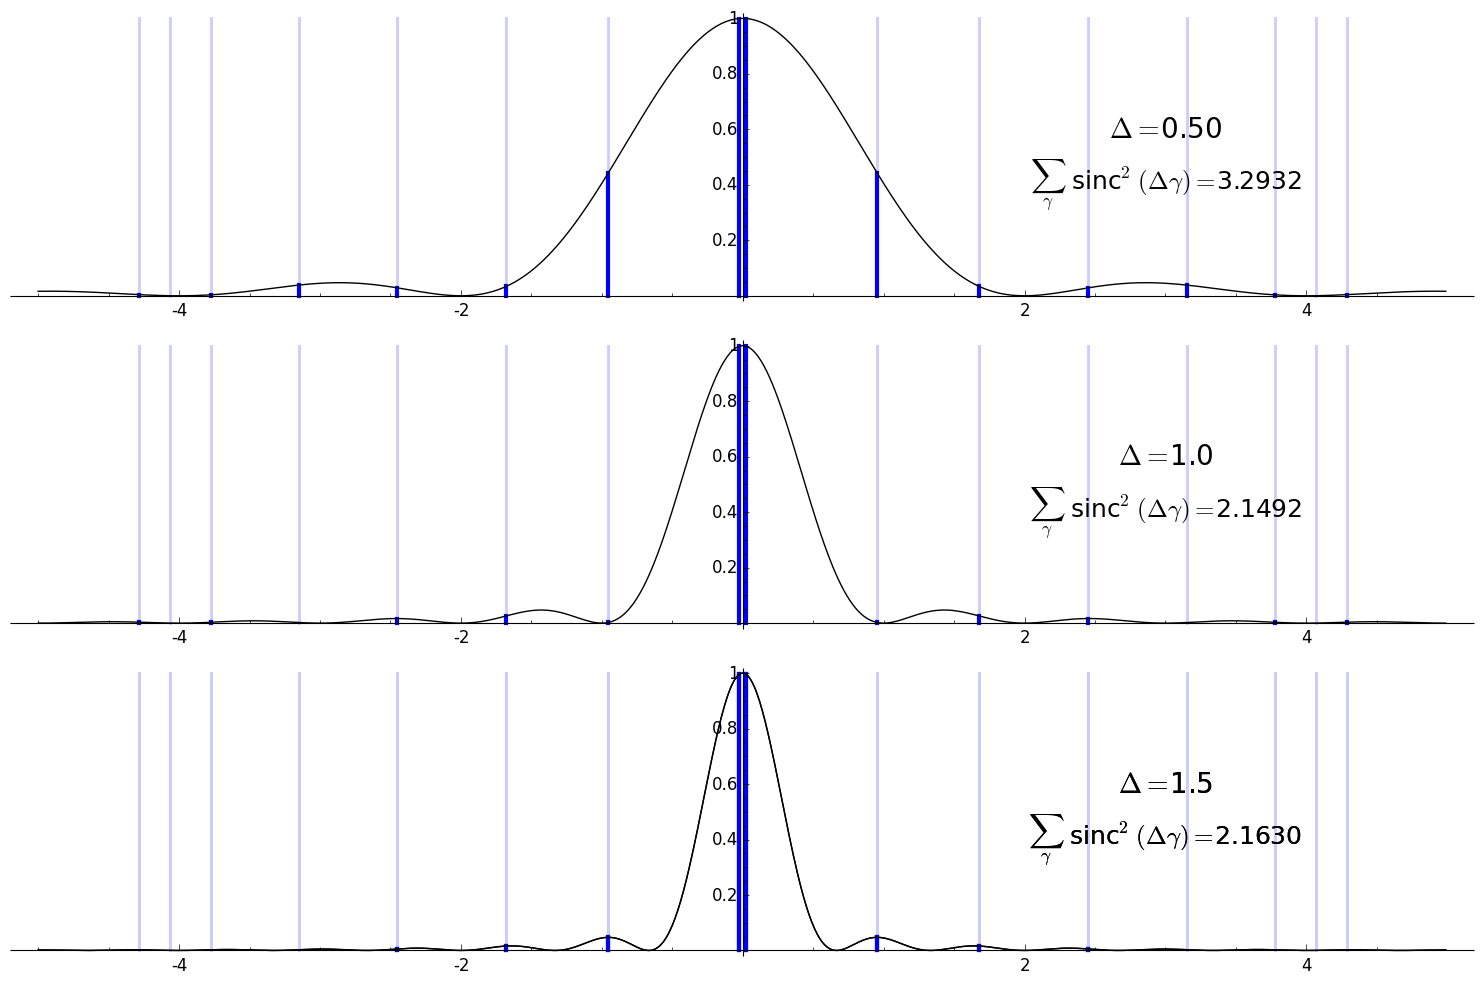
\includegraphics[width=1.0\textwidth]{graphics/256944c1_zero_sum.png}
    \caption{A graphic representation of the $\sinc^2$ sum for the Cremona curve {\tt 256944c1} , a rank 0 curve with conductor $N_E=256944$, for $\Delta = 0.5$, $1.0$ and $1.5$.}
    \label{fig:256944c1_zero_sum}
\end{figure}

However, more work needs to be done regarding the rate of convergence of this sum. We give a result regarding convergence rate of the $\sinc^2$ sum in terms of the bite $\beta_E$ of a curve in Theorem \ref{thm:sinc_squared_sum_with_bite}. However, this is more of a step sideways, as the bite remains a mysterious quantity in its own right. \\

Consider the example in Figure \ref{fig:256944c1_zero_sum}: the Cremona curve {\tt 256944c1}, a rank 0 curve, has a pathologically low-lying zero at $\gamma_0 = 0.02560\ldots$. For small values of $\Delta$, it therefore appears that this curve has analytic rank 2, not zero. In fact, only for $\Delta>\sim 2.815$ does the sum evaluate to a value less than 2 (which, after invoking parity, gives us that it is rank 0). This highlights the fact that some curves -- specifically those with low-lying zeros -- require $\Delta$ to be large for the sum to be within, say, 2 of the true rank of the curve. \\

Furthermore, Figure \ref{fig:256944c1_zero_sum} shows that the convergence from above is unfortunately {\it not} even necessarily monotone: as $\Delta$ is increased the small outlying bumps of the sinc$^2$ function can travel over zeros and temporarily increase the value of the sum. \\

Even though this is the case, we should be able to make some sort of a convexity statement regarding the convergence of the sinc$^2$ sum. This should allow us to use point estimates in the rank estimation code to decide which $\Delta$ values to use on a given curve, and in so doing make the code more efficient. This has the potential to significantly increase the effectiveness of the rank estimation code.

%%%%%%%%%%%%%%%%%%%%%%%%%%%%%%%%%%%%%%%%%%%%%%%%%%%%%%%
\subsection{Better bounds on the bite}

Section \ref{sec:bite} discusses at the topic of the bite of an elliptic curve, namely the quantity
\begin{equation}
\beta_E = \sum_{\gamma \ne 0} \frac{1}{\gamma^2}.
\end{equation}

It would be useful to have better bounds in either direction for this quantity. In terms of bounding from below, we are reasonably confident that the constant $K_{\epsilon}$ in Equation \ref{eqn:bite_lower_bound} can be made explicit in terms of $\epsilon$, given more diligent controlling of the various zero sum-based inequalities. Better yet, it would seem that the bite must grow faster than any multiple of $\log N_E$, and we would like to show that this is the case. It is conceivable that this could also be achieved using the methods detailed in this work. \\

On the other hand, placing an upper bound on the bite is equivalent to bounding the lowest noncentral zero away from the central point. This is a much deeper and more difficult endeavour, equivalent to placing a lower bound on the leading central Taylor coefficient of $\Les$. The latter is done in Chapter \ref{chap:main_theorem}, and in fact a direct corollary of this is that the lowest noncentral zero $\gamma_0$ is bounded below by $(N_E)^{-\alpha}$ for some $\alpha>0$. However, in the leading Taylor coefficient bound a constant introduced from the bound on the real period is never made explicit; while this is good enough to get a polynomial-time rank algorithm out, it {\it isn't} good enough to make the lower bound on $\gamma_0$ explicit. Again, we hope that this issue can be resolved in future work, perhaps by making all constants in bounds on the real period completely explicit.





%%%%%%%%%%%%%%%%%%%%%%%%%%%%%%%%%%%%%%%%%%%%%%%%%%%%%%%
\printendnotes

%
% ==========   Bibliography
%
\nocite{*}   % include everything in the thesis.bib file
\bibliographystyle{acm}
\bibliography{bibliography}
%
% ==========   Appendices
%
\appendix
\raggedbottom\sloppy
 
% ========== Appendix A
 
\chapter{Code Repo and Blog Posts}
 
The analytic rank estimation code mentioned in this thesis is hosted on GitHub, and is accessible to all free of charge under the GNU General Public License.

\begin{itemize}
\item The repo can be found at
\begin{description}
\item[] \verb%https://github.com/haikona/GSoC_2014%
\end{description}
The relevant Sage Trac ticket is
\begin{description}
\item[]\verb%http://trac.sagemath.org/ticket/16773%
\end{description}

\item Moreover, as it was being written the code was blogged about extensively; the posts on various aspects of the code's functionality can be found at
\begin{description}
\item[]  \verb%http://mathandhats.blogspot.com/%
\end{description}

\end{itemize}

\vita{Simon Spicer was born and raised in Johannesburg, South Africa, but has spent the past six years in Seattle pursuing his mathematics PhD at the University of Washington. At the time of completing this thesis he and his wife Kimberly have just welcomed their first child, Bramwell, into the world. In his spare time Simon enjoys writing code, piloting airplanes and attempting to teach his family Afrikaans.}


\end{document}
